\graphicspath{{chapters/analysis/images/}}
\chapter{A Search for Tau Neutrinos from Oscillations}



\label{chapter:analysis}
The GRECO event selection expects tau neutrinos with a rate of 45~$\mu$Hz, corresponding to an expectation about 3000 events over the course of three years.
These events will be used to search for tau neutrino appearance in DeepCore.

The tau neutrino appearance measurement is described in this chapter.
The chapter begins in in Section~\ref{sec:tau_parametrization} with a discussion of how to parametrize the tau neutrino appearance as well as a review of the two previous tau neutrino appearance measurements performed by the OPERA and Super-Kamiokande experiments.

A description of the fitting process follows with descriptions of the systematic uncertainty parametrizations used in Section~\ref{sec:systematics}.
The sensitivity of the measurement is given in Section~\ref{sec:sensitivity}.
The impact of systematic uncertainties on the expected confidence interval is described in Section~\ref{sec:systematics_impact}.

Finally, the results of the analysis are presented in Section~\ref{section:tau_results} before a discussion of complementary oscillation results performed with the GRECO sample.
A short conclusion follows to highlight some possible improvements for future analyses.











\label{sec:tau_parametrization}
\section{Parametrizing the Tau Neutrino Appearance}
In order to measure the appearance of tau neutrino events, a choice of "appearance parameter" must be selected.
Previous analyses have characterized the appearance using a normalization term \cite{SuperK-Tau2013,SuperK-Tau2017,OPERA-Tau2015}.
This approach elegantly encapsulates many possible sources of uncertainty in the tau neutrino sector into a single, measurable value, including non-unitarity, uncertainties in the tau cross section, 

\label{subsec:cc_vs_ccnc}
\subsection{CC vs CC+NC}
As described in \ref{sec:detection_methods}, neutrinos may interact via the charged current and neutral current interactions.
These interactions provide separate windows into the measurement of tau neutrino appearance.
Tau neutrino events may interact in either of these channels depending on the neutrino energy.

With a mass of 1776.82~$\pm$~0.16 MeV and a lifetime of 290.3~$\pm$~0.5 femtoseconds \cite{PDG-2015}, tau leptons from tau neutrino charged current interactions in DeepCore at energies less tha 100 GeV travel distances O(1 mm) before decaying.
The charged current interactions of the tau result in a variety of signatures due to the unique decay behavior of the tau lepton.

\label{eqn:tau_decay_modes}
\begin{equation}
	\tau^- \rightarrow 
		\begin{cases} 
			\mu^- \ \bar{\nu}_\mu \ \nu_\tau & \mbox{17.41 $\pm$ 0.04\%} \\ 
			e^- \ \bar{\nu}_e \  \nu_\tau & \mbox{17.83 $\pm$ 0.04\%} \\ 
			\mbox{Hadrons} & \mbox{Otherwise} \\ 
		\end{cases}
\end{equation}

In either the muonic or the electronic decay modes, a fraction of the energy is lost to outgoing neutrinos, resulting in a smaller observed charge than would be associated with a corresponding interaction of another neutrino type.
Furthermore, the muonic decay mode may lead to a visible muon track for the tau neutrino interaction.
These muon tracks associated with the appearance of tau neutrino would appear at lower energies than the tracks corresponding to the muon neutrino disappearance, allowing both the appearance of tau neutrinos and the disappearance of muon neutrinos to be observed simultaneously.

Unlike charged current interactions, neutral current interactions of neutrinos have identical coupling to the Z boson regardless of flavor and, therefore, undergo no observable change due to unitary oscillations.
Because of this, studies of the standard unitary PMNS matrix treat neutral current events as non-oscillating \cite{SuperK-Tau2013,SuperK-Tau2017,OPERA-Tau2015,IceCube-Oscillation2018}.
In contrast, searches for new physics and sterile neutrinos measure deviations from the expected number of neutral current interactions in the detector \cite{MINOS-SterileNC-2011}.

For this analysis, both channels are used to measure the appearance of tau neutrinos.

\label{subsec:norm_tau}
\subsection{The $\nu_{\tau}$ Normalization}
In the atmospheric neutrino flux, tau neutrinos are only produced directly above energies of a few TeV through the decay of charmed mesons.
Because effectively all tau neutrino events observable in DeepCore are the result of neutrino oscillations, the total number of observed tau neutrino interactions is a direct measure of the appearance.

Following the definition of analyses performed by other experiments \cite{SuperK-Tau2013,SuperK-Tau2017,OPERA-Tau2015}, the tau neutrino normalization, $N_{\nu_\tau}$, is adopted as the primary physics parameter in the search for tau neutrino appearance.
The normalization is defined to be a scaling of the number of expected tau neutrino events after the effects of all systematic uncertainties are applied.
The parameter modifies the number of events expected in each bin 

\label{eqn:norm_tau_definition}
\begin{equation}
	f'_{ijk} = \left( \sum_{m\neq\nu_\tau} f^m_{ijk}\left(\theta_{23}, \Delta m_{32}^2, ...\right) \right) + N_{\nu_\tau} f^{\nu_\tau}_{ijk}\left(\theta_{23}, \Delta m_{32}^2, ...\right) 
\end{equation}

where $f^m_{ijk}$ is the expected rate in bin $ijk$ from a particle type 

\begin{equation}
m=(\nu^{CC}_e, \nu^{CC}_\mu, \nu^{CC}_\tau,\nu^{NC}, \mu_{Atm}, Accidental) .
\end{equation}

A value of $N_{\nu_\tau}=1.0$ indicates that the number of events is consistent with the number expected assuming unitary oscillations and the GRV98NLO cross section model in the GENIE generator.
If the value differs significantly from 1.0, it may be indicative of either mismodeled cross-sections \cite{Description-DsTau,SuperK-Tau2017} or of novel physics\cite{Tau-NuDecay}. 
Due to the large existing uncertainties in the PMNS matrix described in \ref{subsec:steriles_unitarity}, either situation is likely to yield valuable information.


\label{subsec:superk_and_opera}
\subsection{Limits on the Tau Neutrino Normalization}
This analysis is not the first to search for tau neutrino appearance.
Two other experiments, OPERA and Super-Kamiokande, have reported previous measurements parametrized in the same way.

\label{subsubsec:opera_limit}
\subsubsection{The OPERA Limit}
The \emph{Oscillation Project with Emulsion-tRacking Apparatus,} better known by the acronym \emph{OPERA}, is an experiment designed to search for tau neutrino appearance \cite{Description-OPERA}.
Unlike IceCube's use of atmospheric neutrinos, OPERA uses muon neutrinos produced in the CERN Neutrinos to Gran Sasso (CNGS) beamline.
OPERA uses bricks of emulsion cloud chambers in order to accurately track and reconstruct neutrino interactions in the fiducial volume.
This technique allows analyzers to identify not only the initial neutrino interaction vertex, but also the decay products along the path of the charged lepton produced in charged current interactions.
An example of one tau neutrino event observed is shown in Figure~\ref{fig:opera_event}.
In OPERA, the tau lepton produced during a tau neutrino charged current interaction decays, produceing a characteristic kink visible in the detector that can be used to identify tau neutrino candidate events.
The ability to identify the particle dynamics is balanced by the small fiducial volume of the experiment, yielding only 5408 useful events for analysis from five years of data-taking \cite{OPERA-Tau2015}.

\begin{figure}
\centering
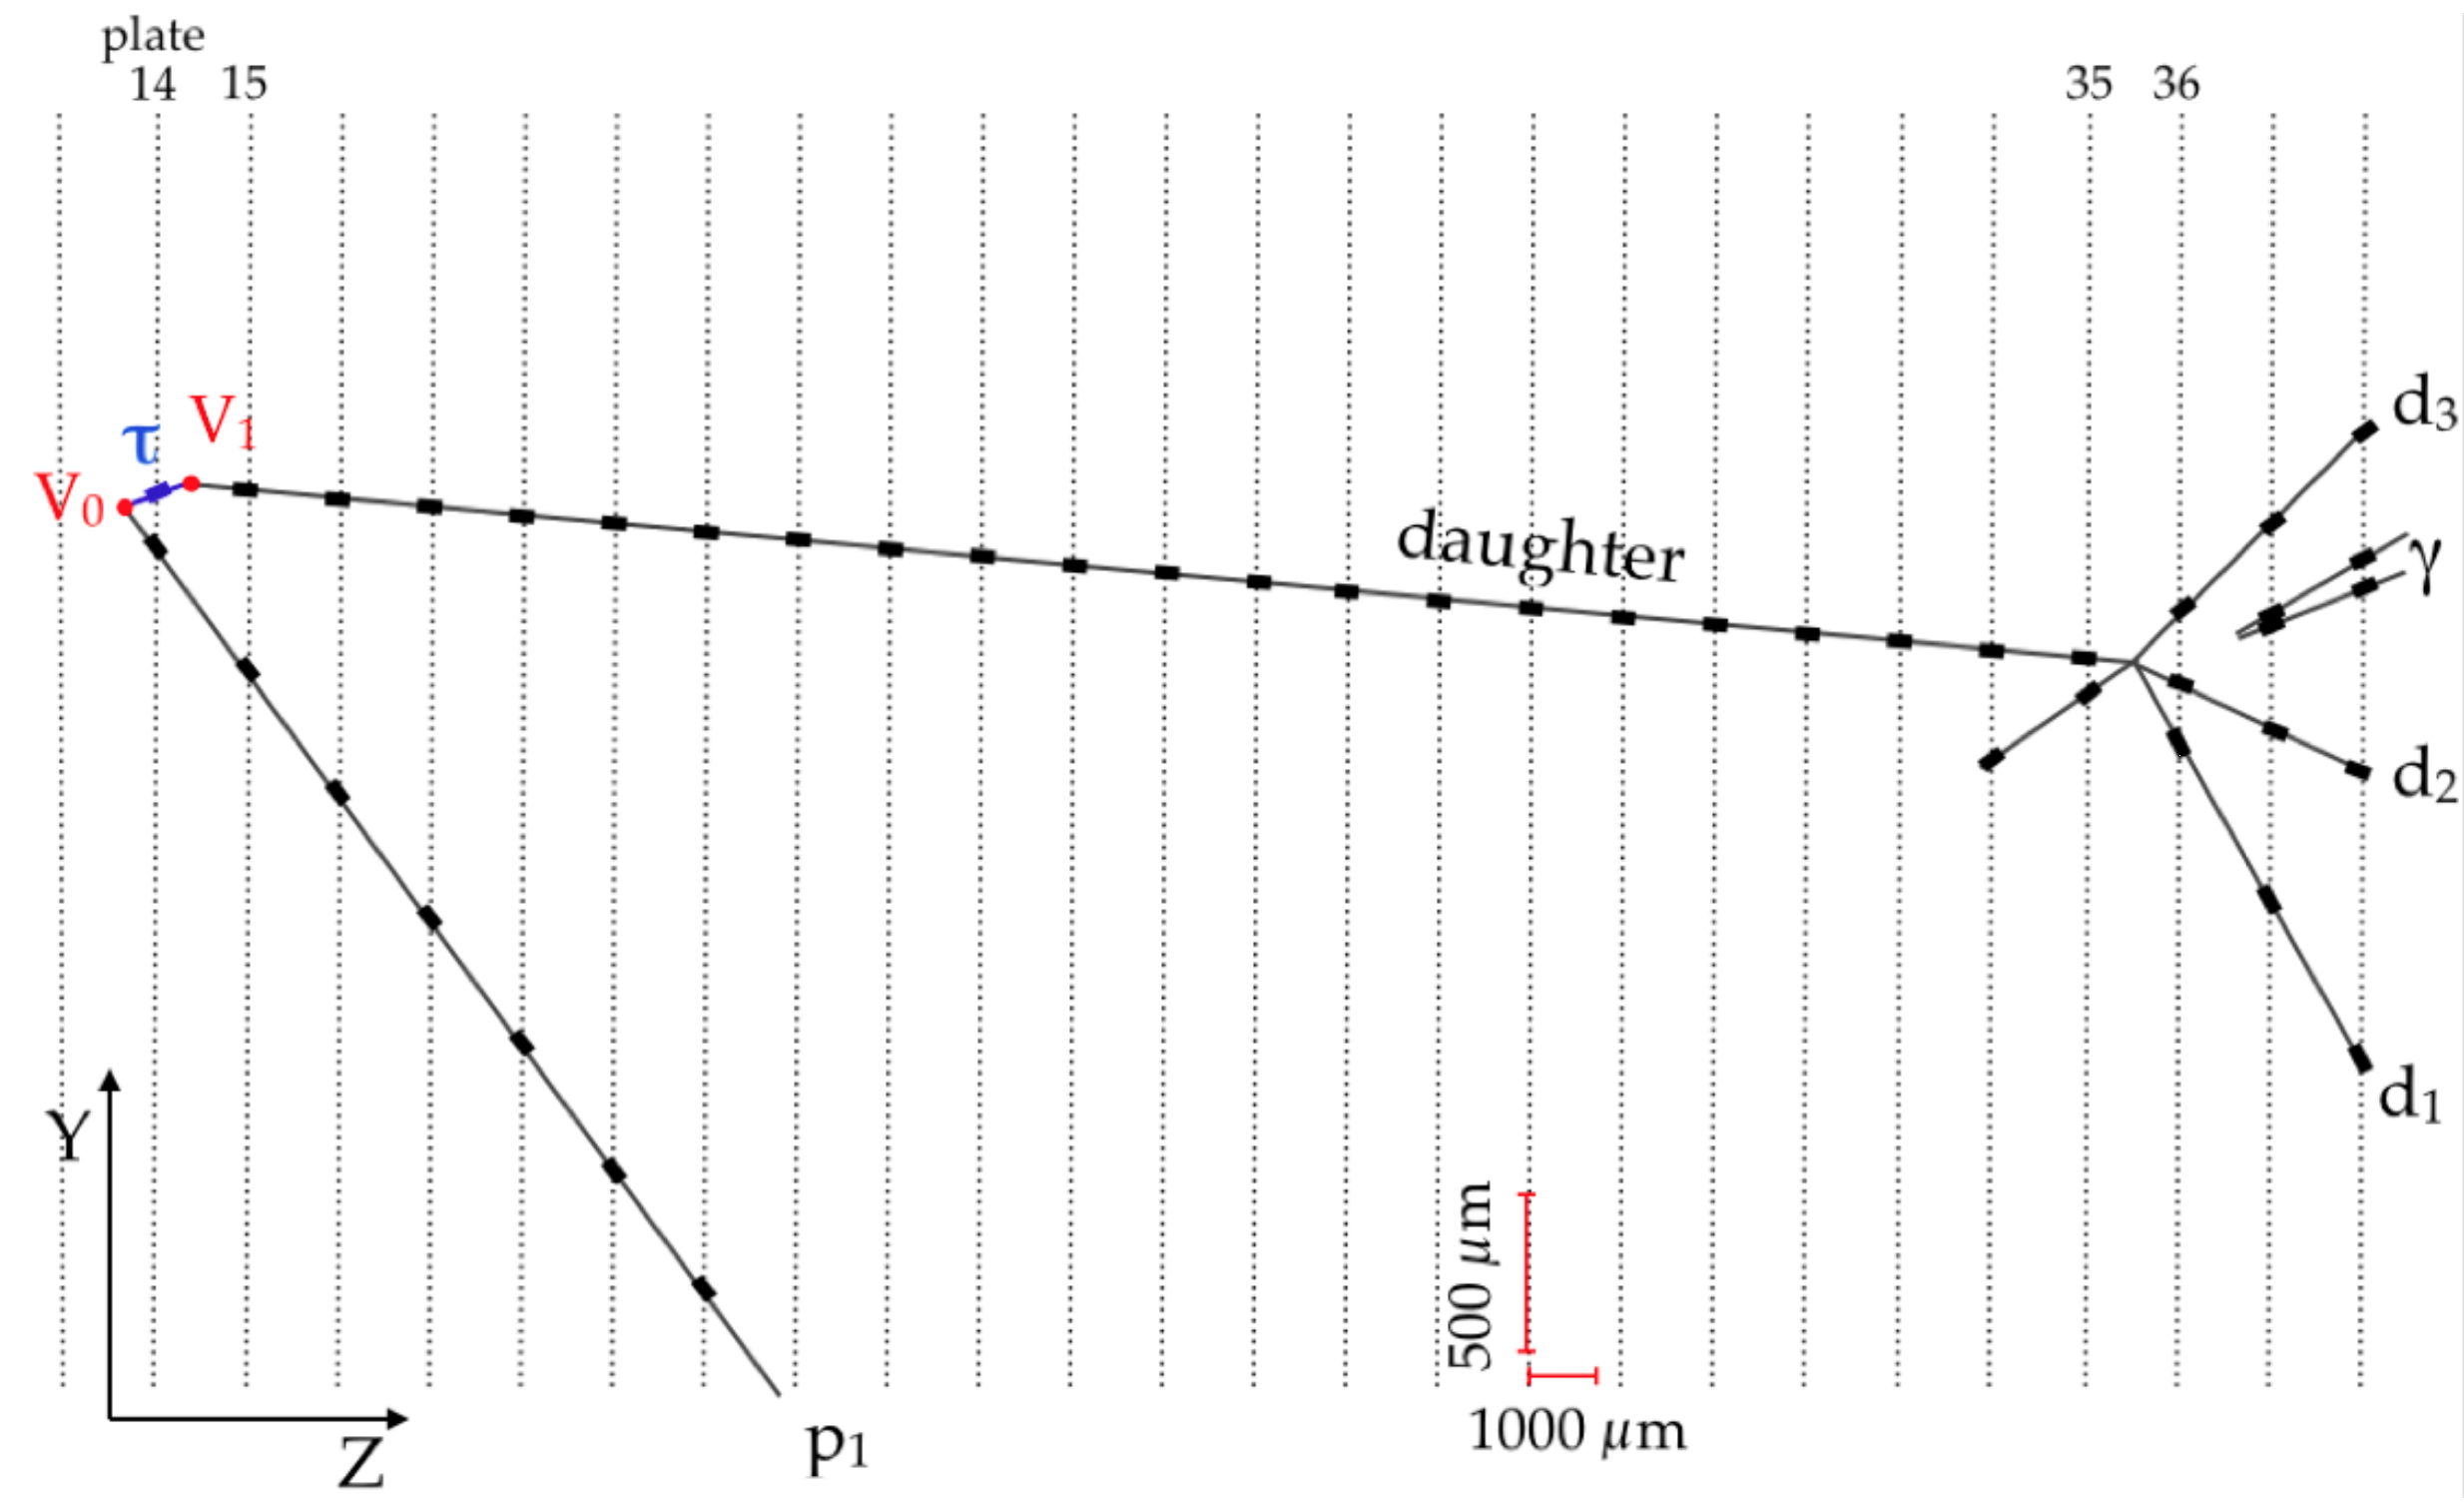
\includegraphics[width=0.7\textwidth]{OPERA_event5.png} 
\caption[A tau neutrino event observed at OPERA]{An event display of the reconstructed interaction of a tau neutrino interaction in the OPERA detect. The initial interaction vertex, $V_0$, produces a tau lepton, shown in blue. The OPERA detector's micrometer spatial resolution enables the identification of individual tau neutrino interactions. Figure from \cite{OPERA-Tau2015}.}
\label{fig:opera_event}
\end{figure}

In 2015, OPERA Collaboration released the final result in their search for tau neutrino appearance using charged current interactions.
Five candidate events were identified in the data sample with a signal expectation of 2.64 $\pm$ 0.53 and a background expectation of 0.25 $\pm$ 0.05.
The data unambiguously rules out the no-appearance hypothesis, with a rejection at 5.1$\sigma$.

OPERA reported a final value of $N^{CC}_\tau=1.8^{+1.8}_{-1.1}$ at the 90\% confidence level. 
This value is consistant with the standard unitary oscillation scheme, but with large errors.

\label{subsubsec:superk_limit}
\subsubsection{The Super-Kamiokande Limit}
Super-Kamiokande, described in Section~\ref{sec:superk_atmo}, also has reported results in searches for tau neutrino appearance.
The Super-Kamiokande collaboration developed an event selection in the search for tau neutrino events, including the implementation of a neural network trained to identify tau-like and non-tau-like events \cite{SuperK-Tau2013,SuperK-Tau2017}.
Events are analyzed in terms of the zenith angle and the neural network output variable.

\begin{figure}[h]
\centering
\begin{tabular}[b]{c}
  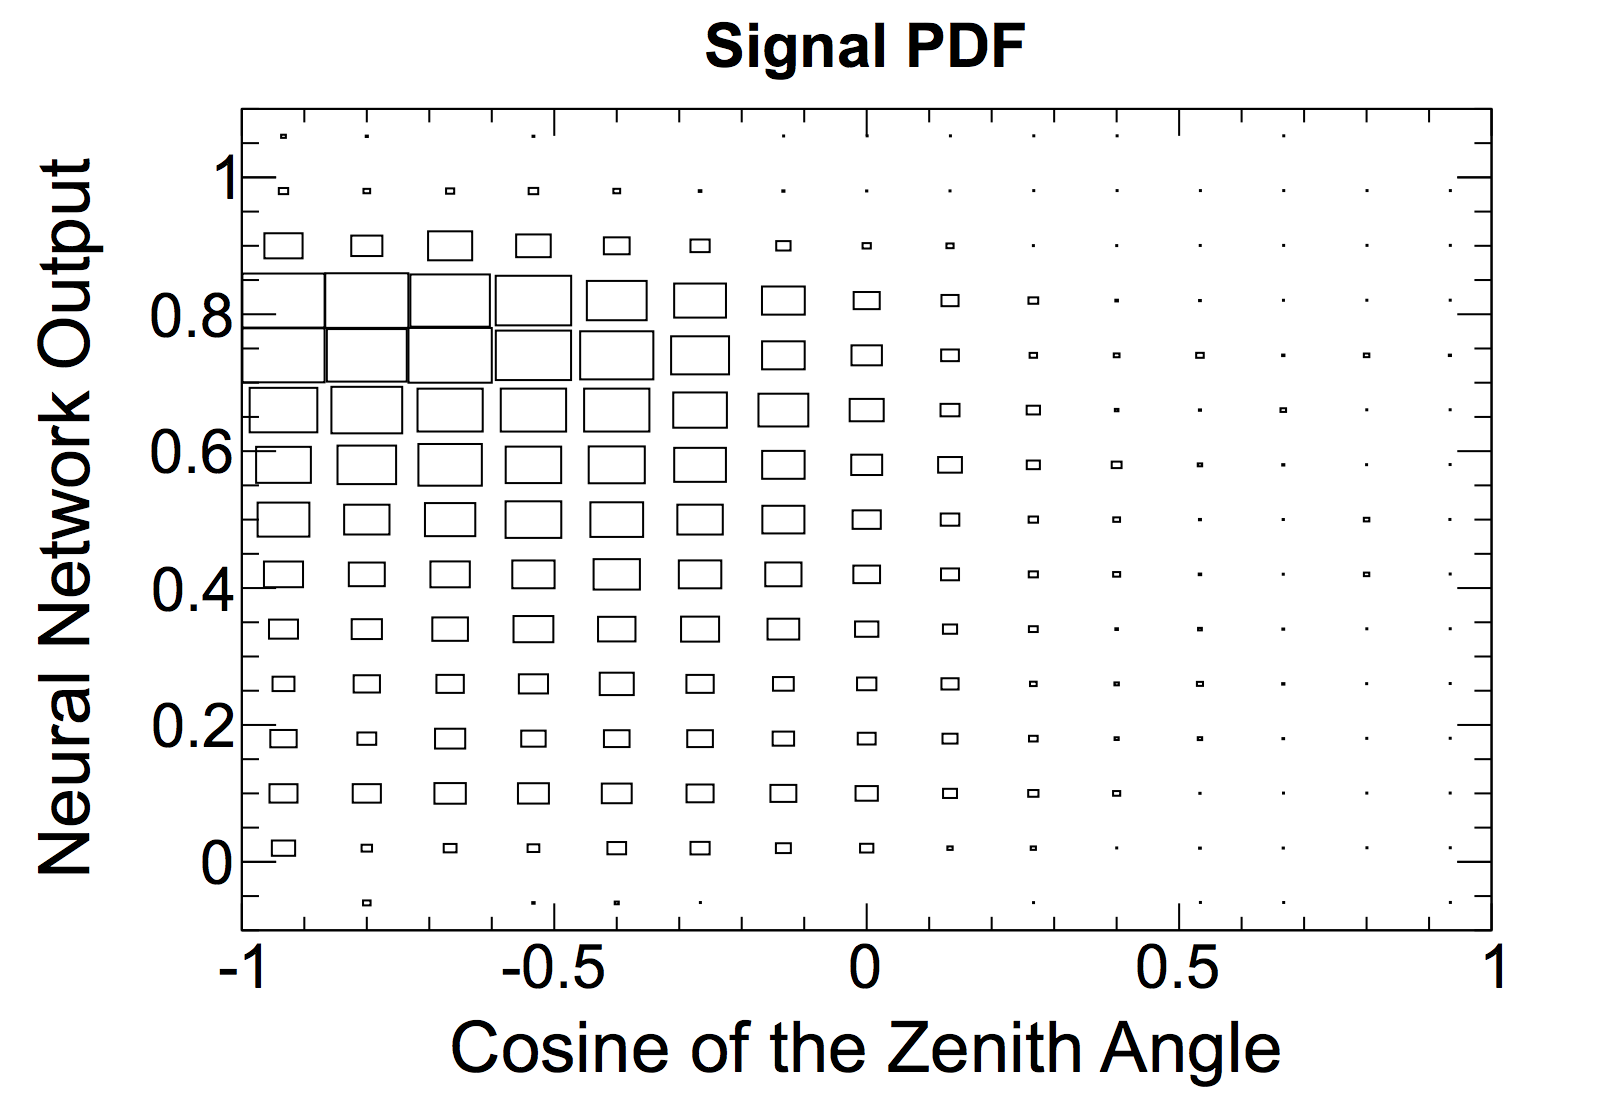
\includegraphics[width=0.45\linewidth]{superk_signal.png} \\
  \small (\textbf{\color{ctcolormain}a}) SuperK Signal Template
\end{tabular} \hspace{2pt}
\begin{tabular}[b]{c}
  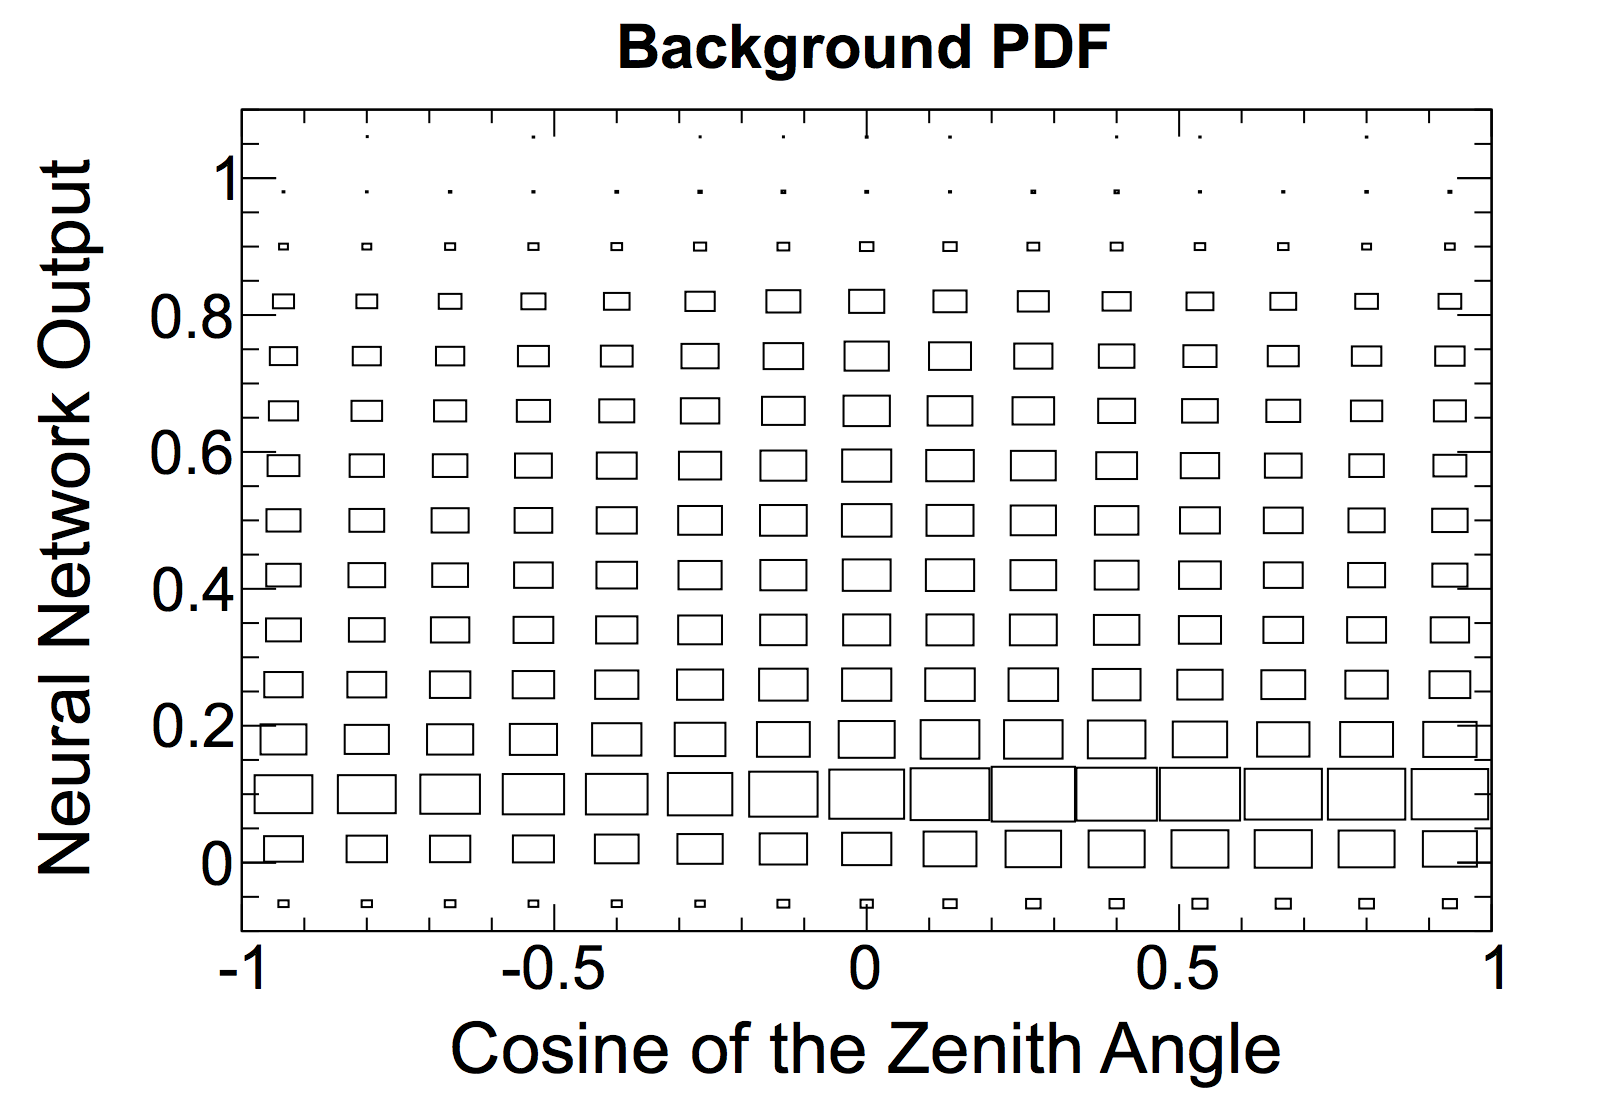
\includegraphics[width=0.45\linewidth]{superk_background.png} \\
  \small (\textbf{\color{ctcolormain}b}) SuperK Background Template
\end{tabular}
\caption[Signal and background in the Super-Kamiokande analysis]{The signal (a) and background (b) histograms used in the Super-Kamiokande search for tau neutrino appearance. The data is binned to show the location of events, although the fit is performed using an unbinned likelihood. The signal tau neutrino events appear in the upgoing region. Image from \cite{SuperK-Tau2017}.}
\label{fig:superk_histograms}
\end{figure}

The background and signal event distributions, shown in Figure~\ref{fig:superk_histograms} are fit to 5326 days of atmospheric neutrino data with an unbinned likelihood with 28 systematic uncertainties included in the analysis.

\begin{table}[]
\centering
\begin{tabular}{@{}llll@{}}
\toprule
Interaction Mode & Non-tau-like & tau-like & All    \\ \midrule
CC nue       & 3071.0          & 1399.2      & 4470.2 \\
CC numu     & 4231.9          & 783.4       & 5015.3 \\
CC nutau    & 49.1            & 136.1       & 185.2  \\
NC               & 291.8           & 548.3       & 840.1  \\ \bottomrule
\end{tabular}
\caption[The rates expected for each of the neutrino types in the Super-Kamiokande search for tau neutrino appearance]{The rates expected for each of the neutrino types in the Super-Kamiokande search for tau neutrino appearance. Reproduced from \cite{SuperK-Tau2017}.}
\label{tab:superk_appearance_rates}
\end{table}

The expected rates of the Super-Kamiokande analysis are shown in Table~\ref{tab:superk_appearance_rates}.
The Super-Kamiokande measurement yields an expectation of 185.2 tau neutrino events in 5326 days or approximately 12.7 events per year.
After fitting, the final rejection of the no-appearance hypothesis, $N^{CC}_\tau$=0, is found to be 4.6$\sigma$.
Like OPERA, Super-Kamiokande finds more tau neutrino candidate events than expected, with a best-fit normalization of $N^{CC}_\tau=1.47~\pm~0.32$ at the 68\% level.





















\label{sec:binning}
\section{Binning of the Appearance Analysis}
The signature of tau neutrino appearance in DeepCore is an energy and zenith angle dependent excess of cascade-like events. 
To measure the appearance signature, a binned likelihood, described in \ref{sec:likelihood}, is used to fit the simulation to the data.
The analysis uses two variables to describe the oscillations: the reconstructed energy and zenith angle.

The choice of binning for zenith angles is selected to be similar, but somewhat finer than previous work and uses the full sky \cite{IceCube-Oscillation2013,IceCube-Oscillation2015,IceCube-Oscillation2018}.
The upgoing events (${cos(\phi)}=-1$) pass through the full diameter of the Earth where we expect the strongest oscillation effects while the downgoing events (${cos(\phi)}=1$) originate in showers above the Antarctic.
The energy binning is identical to previous oscillation analyses from DeepCore and consists of 8 bins logarithmically spaced from 5.6 GeV to 56 GeV, avoiding potential problems due to disagreements at high energies discussed in Section~\ref{subsec:bedrock}.

\label{sec:pid_variables}
\subsection{Particle ID Variables}
Separating the sample into cascade-like and track-like events provides better sensitivity than using solely track-like events \cite{IceCube-Oscillation2015,IceCube-Oscillation2018,IceCubeSterile-Andrii,SuperK-Tau2017}.
A separation of this type, referred to as a \emph{particle identification} variable (\emph{PID}), allows the disappearance and appearance effects to be observed independently and provides a stronger limit on uncertainties from systematic effects.
Two such variables are available in the GRECO sample, shown in Figure~\ref{fig:pid_variables}.

\begin{figure}[h]
\centering
\begin{tabular}[b]{c}
  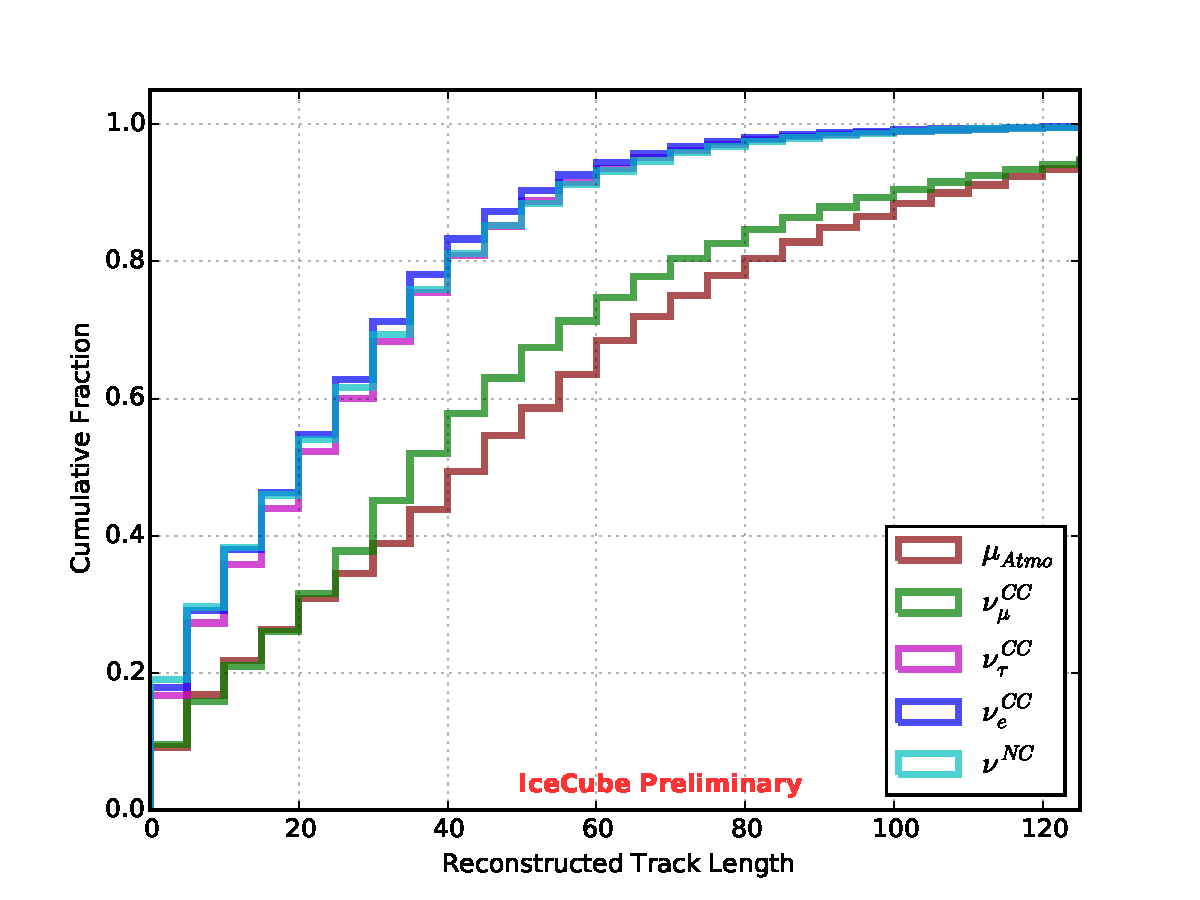
\includegraphics[width=0.45\linewidth]{track_length.pdf} \\
  \small (\textbf{\color{ctcolormain}a}) Reconstructed Track Length
\end{tabular} \hspace{2pt}
\begin{tabular}[b]{c}
  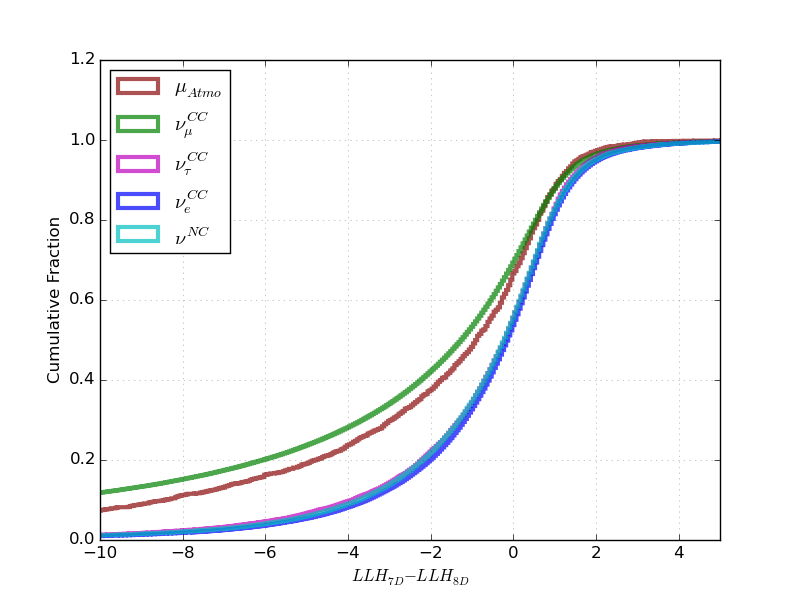
\includegraphics[width=0.45\linewidth]{dLLH.png} \\
  \small (\textbf{\color{ctcolormain}b}) Likelihood Ratio
\end{tabular}
\caption[Cumulative distributions of two PID variables in GRECO]{The cumulative distributions of two variables to separate track-like events (muon neutrino charged current, atmospheric muons) from the cascade-like events (neutral current,electron neutrinos, and tau neutrinos). Larger distances between the muon neutrino charged current and the tau neutrino charged current curves indicates better separating power.}
\label{fig:pid_variables}
\end{figure}

The first PID candidate variable, the reconstructed length of a muon track, provides separation between events with a clear muon track from those without one.
This leads to reasonable separation between the $\nu_\mu$ events undergoing disappearance and $\nu_\tau$ events undergoing appearance.
This may be seen in Figure~\ref{fig:pid_variables}a, where the cumulative distribution of the various simulation components are shown as a function of the reconstructed track length.
The optimal separation between the $\nu_\mu$ and $\nu_\tau$ charged current samples occurs between 30-50 meters.
By separating the sample into cascade-like events (eg. L < 50 m) and track-like events (L $\geq$ 50 m), the disappearance and appearance may be partially disentangled.

The second potential PID variable is the likelihood ratio between PegLeg's mixed cascade+track reconstruction and an analogous cascade-only reconstruction performed using the same tools.
A higher likelihood (lower log-likelihood) in the casade fit implies that the event is more likely intrinsically cascade-like while the reverse is true for intrinsically track-like events.
The information contained in the likelihoods of both fits may be combined to form a likelihood ratio, typically expressed in terms of the log-likelihoods.

\begin{equation}
	\Delta LLH = Log_{10} R_{L} = Log\left(L_{Cascade}\right) - Log\left(L_{Pegleg}\right)
\end{equation}

The cumulative plot of the likelihood ratio is shown in Figure~\ref{fig:pid_variables}b. 
There exists a broad choice of values with similar separation properties from approximuately $-4 < \Delta LLH < -2$.
Once again, separating events into two samples using the likelihood ratio may improve the ability of the analysis to disentangle the disappearance and appearance effects.

\begin{figure}
\centering
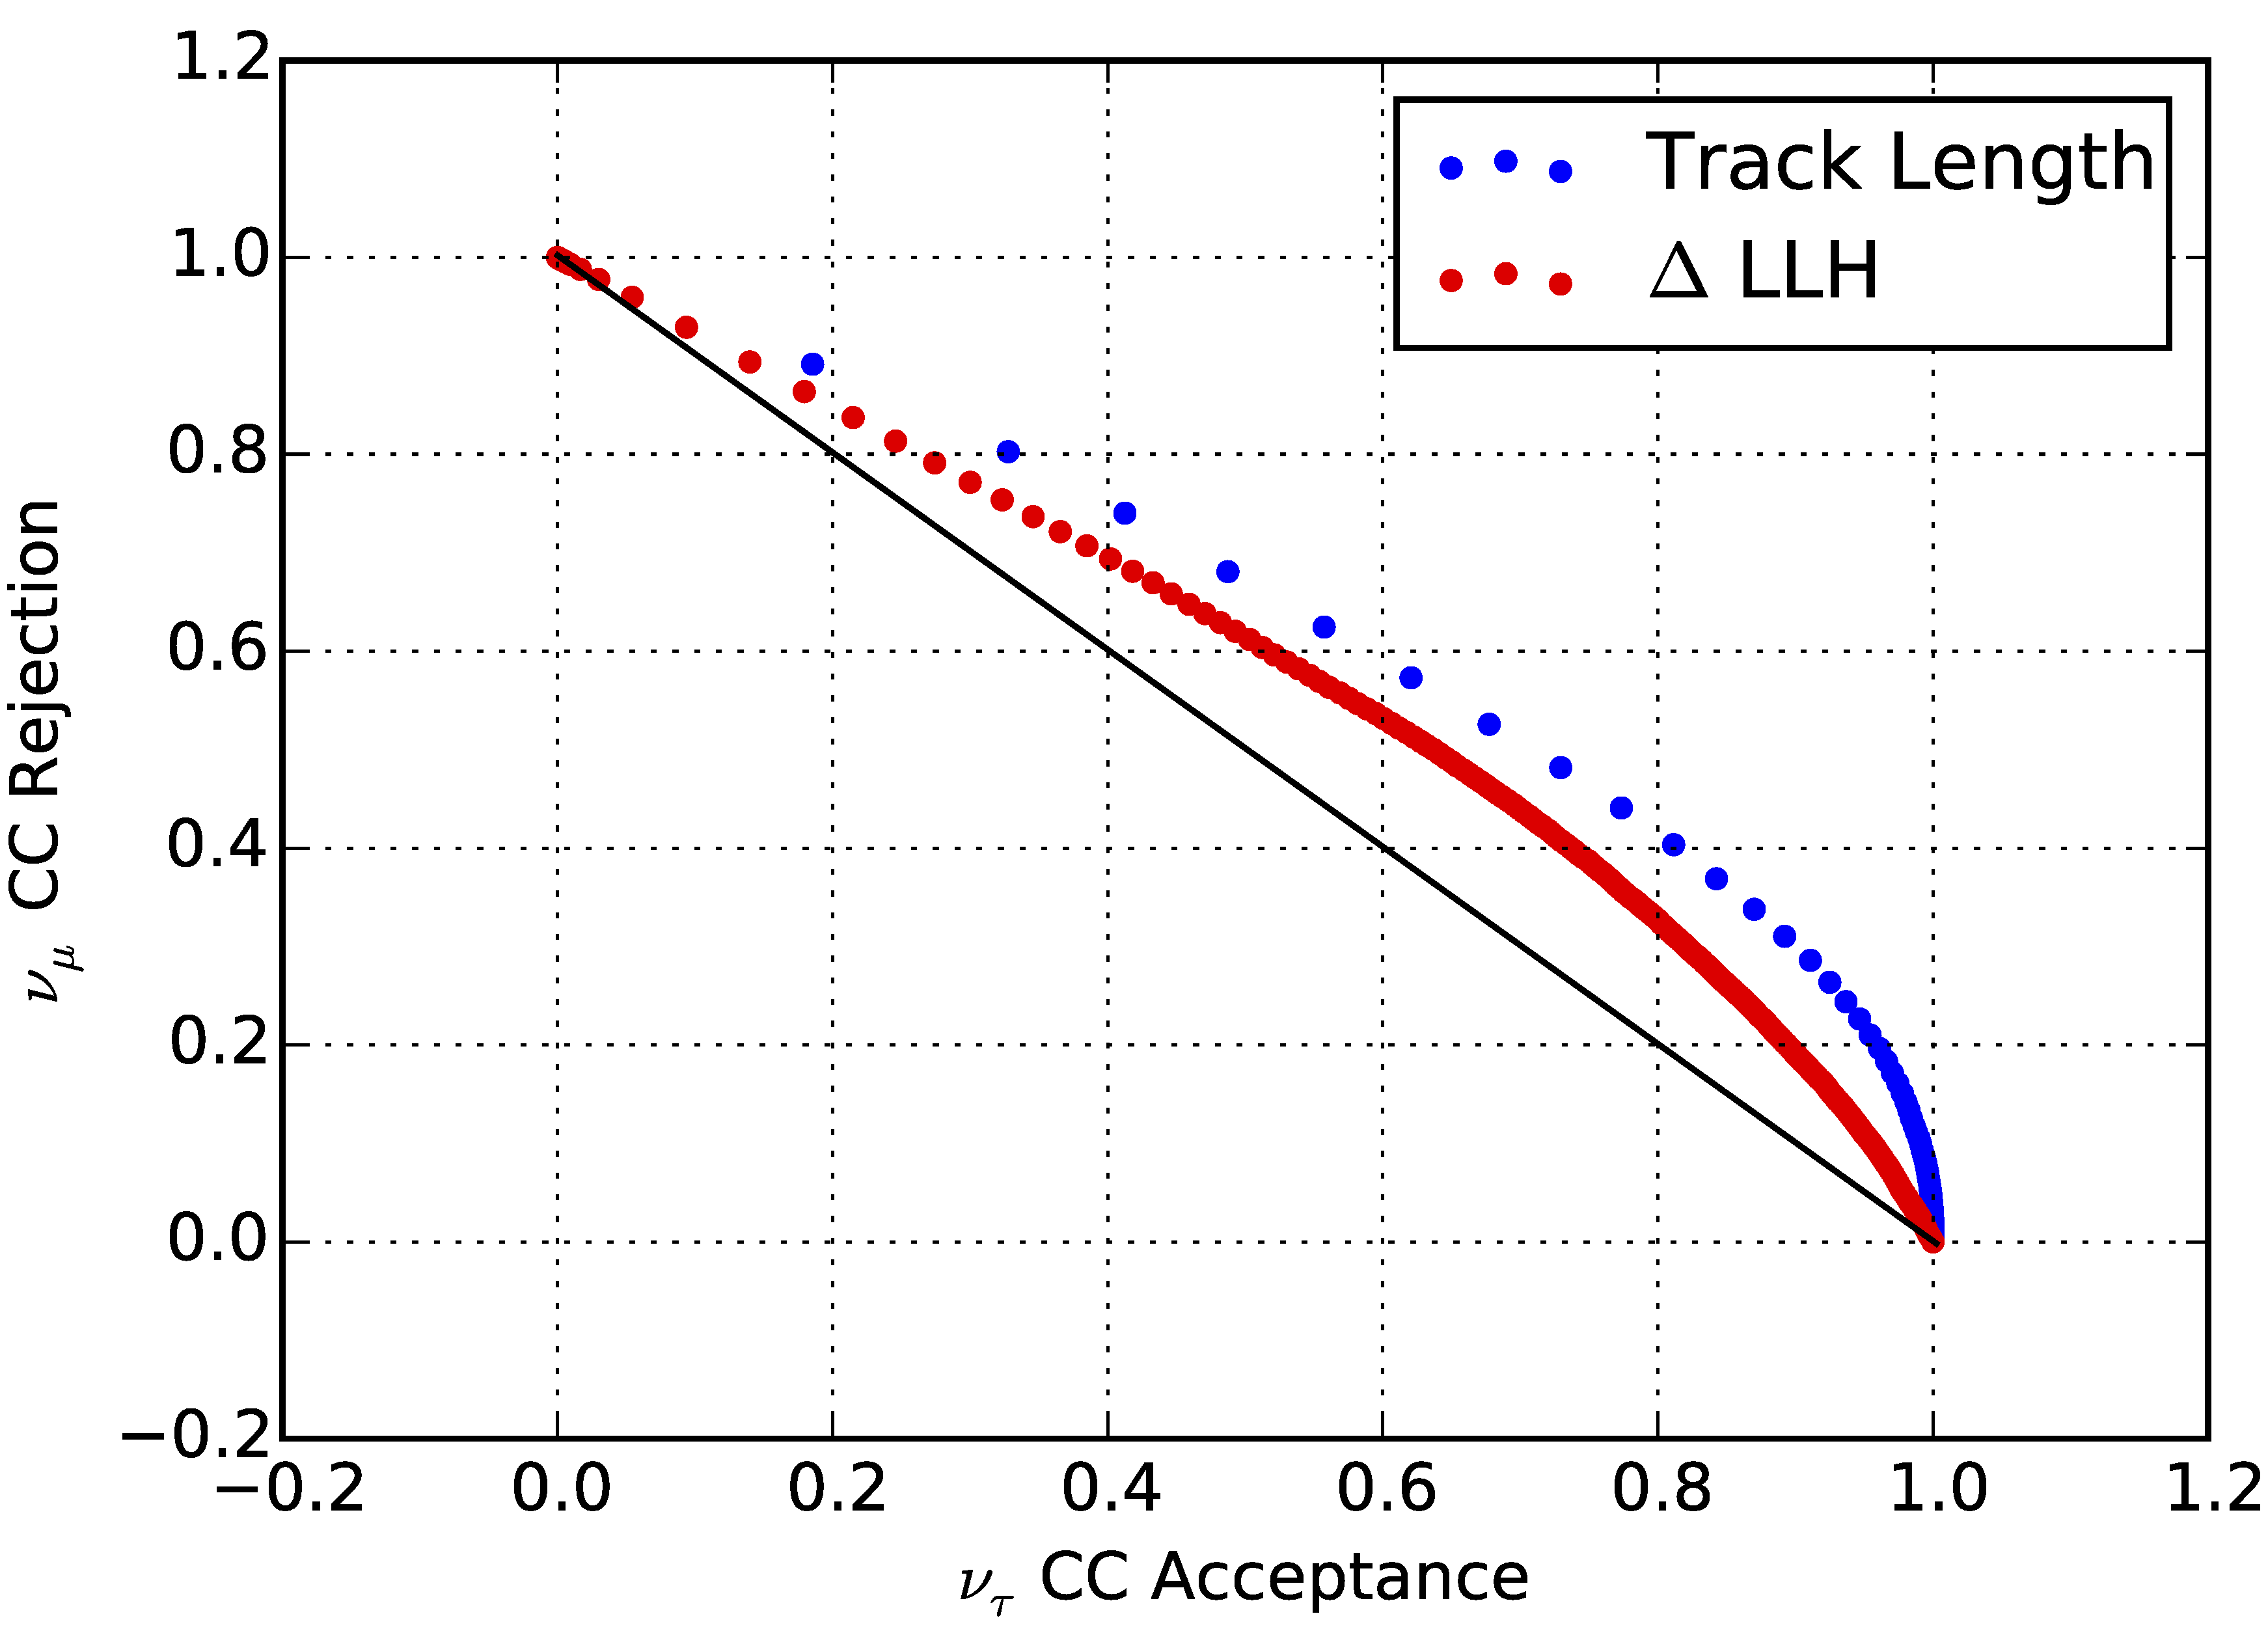
\includegraphics[width=0.7\textwidth]{roc_curves.png} 
\caption[Comparison of separating power between PID variables]{A comparison of the separating power between the reconstructed track length and the likelihood ratio. Each point represents one possible choice of separation value from Figure~\ref{fig:pid_variables}. Points further from the black line indicate stronger separating power between the muon neutrino and tau neutrino charged current events.}
\label{fig:roc_curves}
\end{figure}

An event with a longer reconstructed muon track should be expected to prefer the PegLeg reconstruction over a cascade-only reconstruction.
In order to choose between the parameters, the efficacy of separating each of the simuluation samples from the tau neutrino charged current signal was evaluated.
The results are shown in Figure~\ref{fig:roc_curves}, which give the fraction muon neutrino events rejected and the number of tau neutrino events accepted into the "cascade-like" sample for various choices of the PID values. 
Values further from a diagonal indicate better separation between the muon and tau neutrino events.
The track length performs uniformly better than the likelihood ratio in separating the disappearing muon neutrino charged current and appearing tau neutrino charged current events.
The reconstructed track length is therefore selected as the PID variable for this analysis.

A choice of 50~meters of reconstructed track length is selected to separate the GRECO events into track-like (L~$\geq$~50~m) and cascade-like (L~<~50~m)event samples. 
Because the PegLeg reconstructed energy includes a contribution from the muon track, the division of the sample has an effect on the minimum energy of track-like events.
Using Equation~\ref{eqn:pegleg_energy}, the minimum energy of track-like events with no cascade energy and L~$\geq$ 50~m is 11~GeV.
Track-like events are kinematically limited from reconstructing with energies below this threshold.
Both track- and cascade-like events may reconstruct with higher energies than 10 GeV.


\label{subsec:fit_templates}
\subsection{The MC Fit Templates}
The binned expectations used in the fit for tau neutrino appearance are shown in Figures~\ref{fig:nu_templates} and \ref{fig:bg_data_templates}.
Neutrino histograms assume the oscillation parameters given by the Nu-Fit global fits in Section~\ref{subsec:global_fits} \cite{NuFit.org}.

Muon neutrino charged current events are the dominant component of both the track-like and the cascade-like histograms.
The track-like muon neutrino charged current histogram shows a deficit of events in the upgoing region at an energy of $10^{1.3}=20$~GeV due to muon neutrino disappearance.
The disappearance of muon neutrino events is visible in the track-like channel of both the muon neutrino charged current and the data histograms.

The tau neutrino events appear primarily in the cascade-like histogram.
The signal $\nu_\tau$ events occur in the very upgoing cascade channel and make up, at most, approximately 10\% of the events in those bins.

\begin{figure}[h]
\centering
\begin{tabular}[b]{c}
  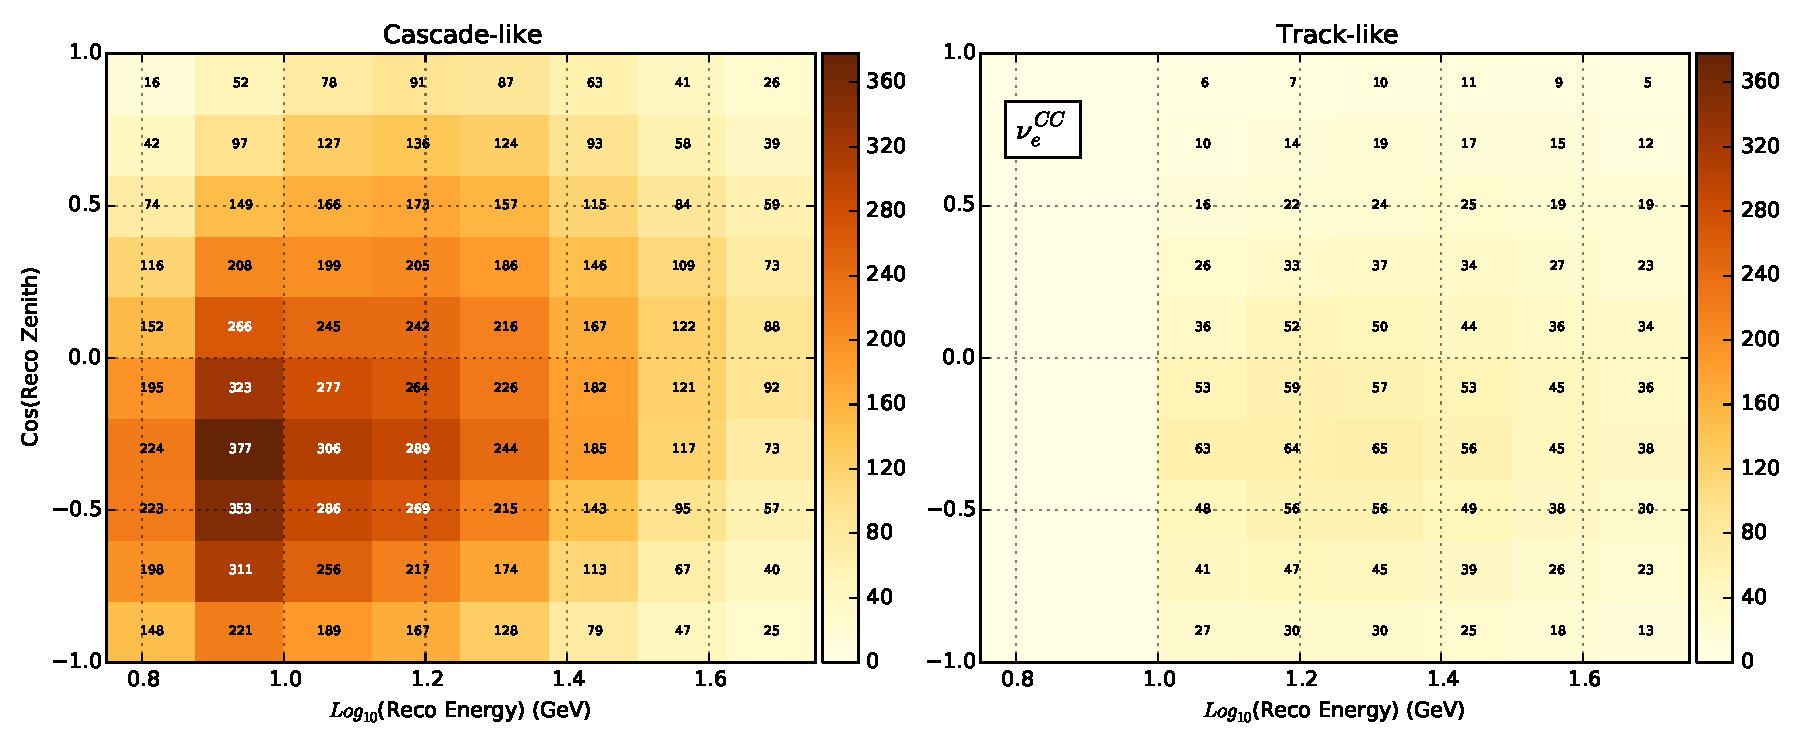
\includegraphics[width=0.7\textwidth]{templates/genie12640(cc).pdf}  \\
  \small (\textbf{\color{ctcolormain}a}) $\nu^{CC}_e$
\end{tabular}
\linebreak
\begin{tabular}[b]{c}
  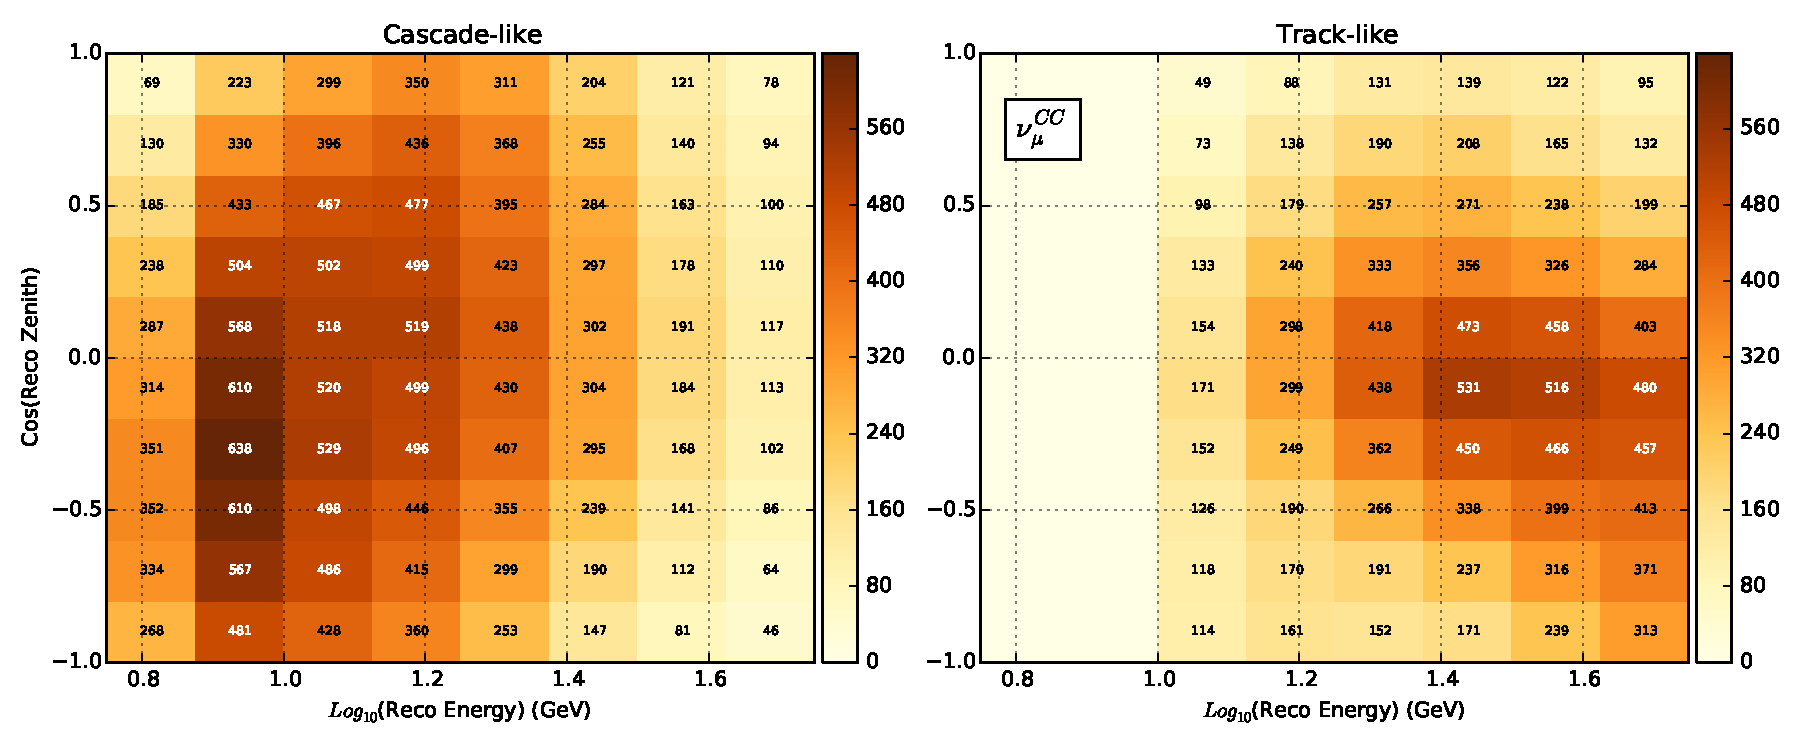
\includegraphics[width=0.7\textwidth]{templates/genie14640(cc).pdf}  \\
  \small (\textbf{\color{ctcolormain}b})  $\nu^{CC}_\mu$
\end{tabular}
\linebreak
\begin{tabular}[b]{c}
  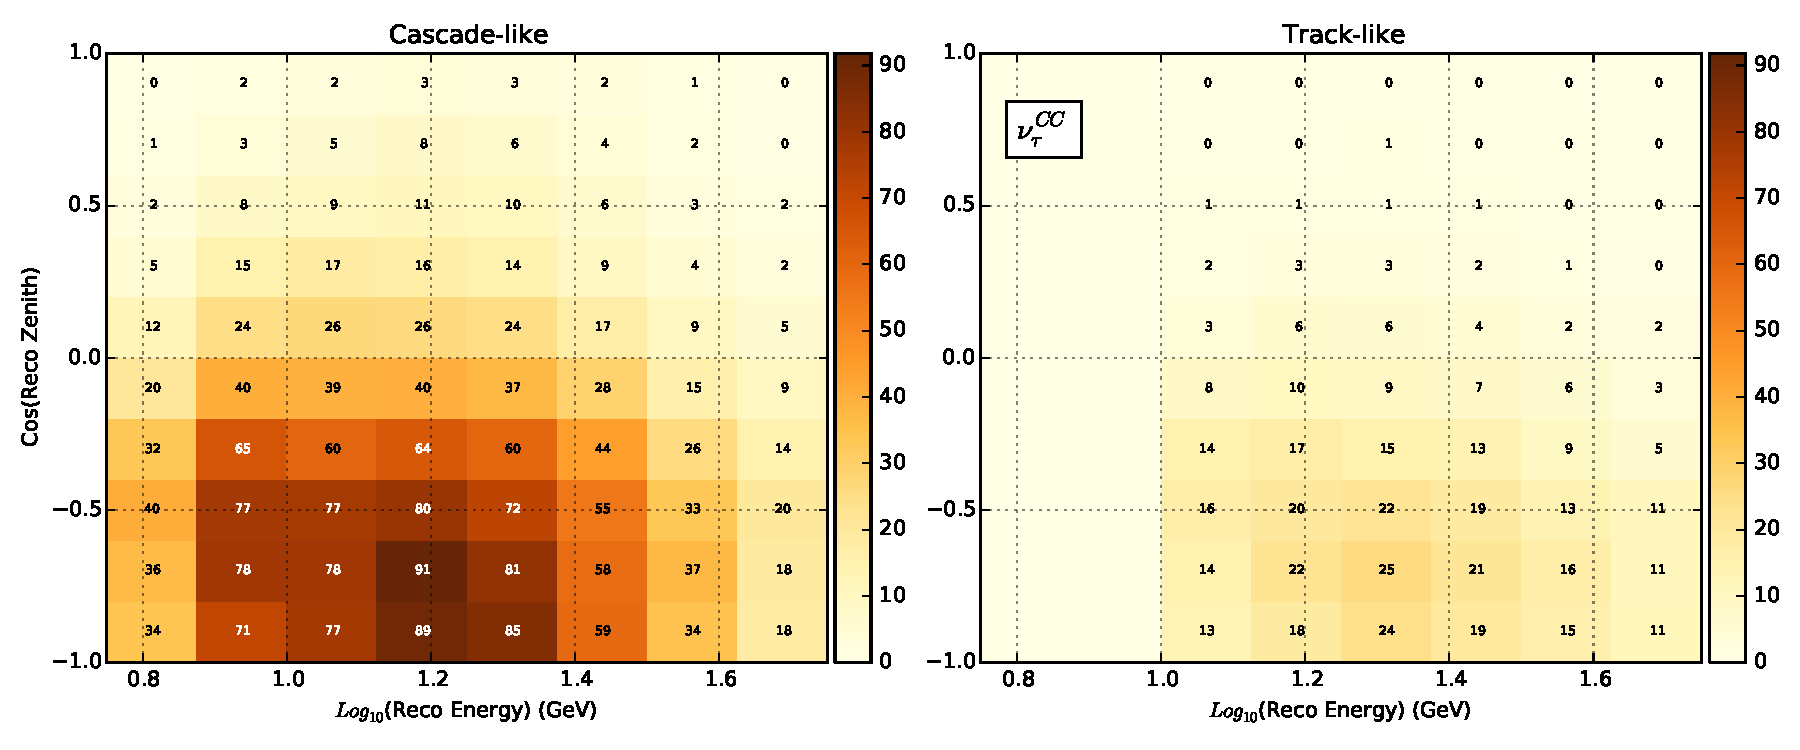
\includegraphics[width=0.7\textwidth]{templates/genie16640(cc).pdf}  \\
  \small (\textbf{\color{ctcolormain}c})  $\nu^{CC}_\tau$
\end{tabular}
\linebreak
\begin{tabular}[b]{c}
  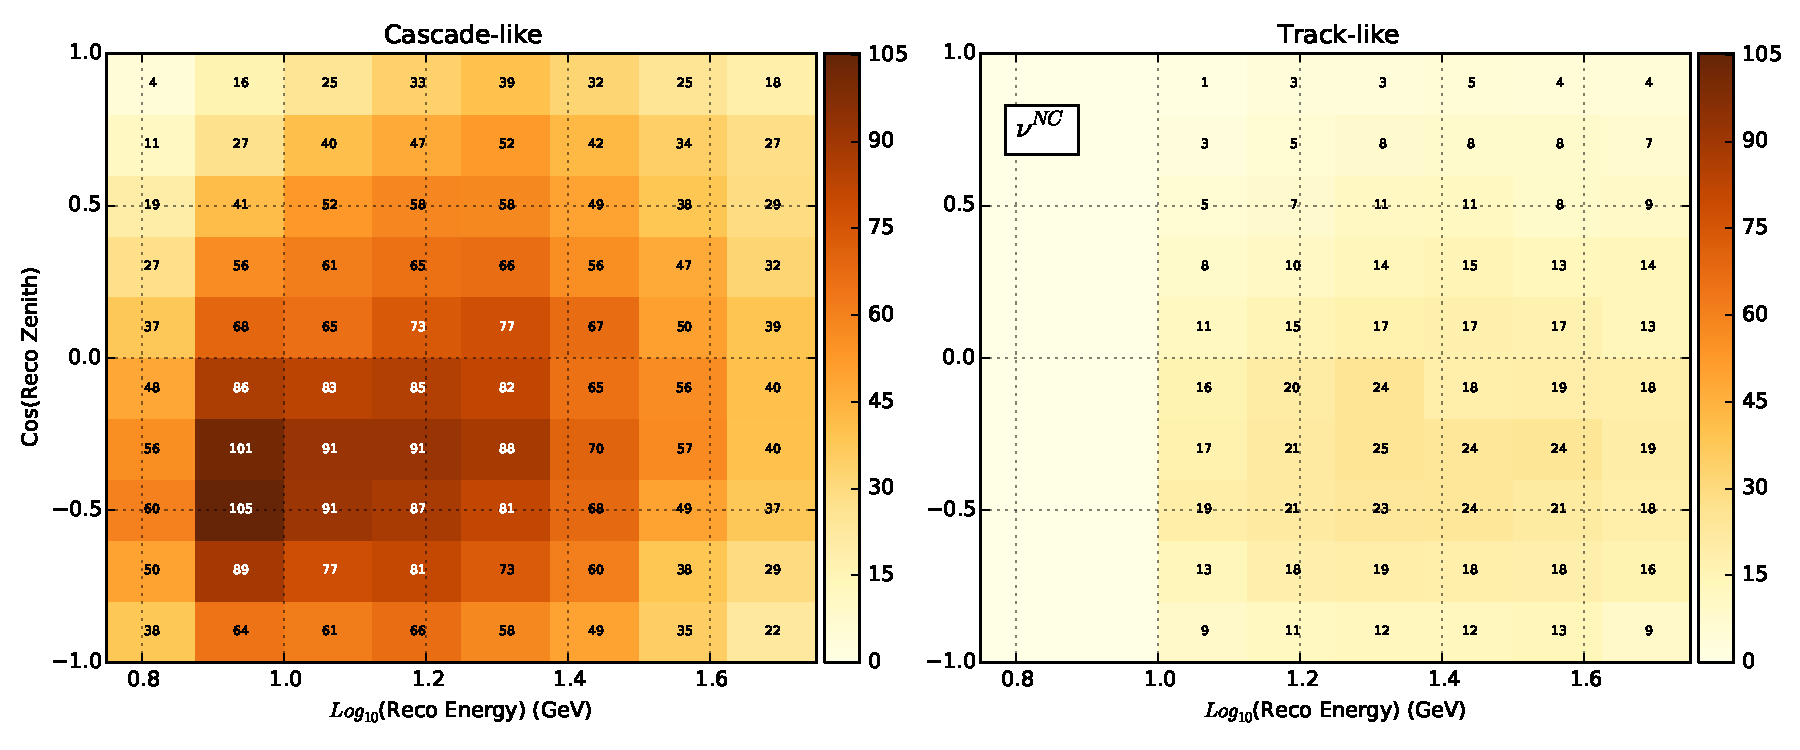
\includegraphics[width=0.7\textwidth]{templates/genie1x640(nc).pdf}  \\
  \small (\textbf{\color{ctcolormain}d})  $\nu^{NC}$
\end{tabular}
\caption[Neutrino histograms for appearance analysis]{The neutrino histograms used in the fit for appearance. The colorbar shows the expected rate from the 3 year sample used in this thesis. The disappearance in the muon neutrino events is visible in the upgoing ($cos(\theta)$=-1) track-like histogram around an energy of $10^{1.3}$=20~GeV. The appearance of tau neutrinos is primarily concentrated in the cascade-like histogram.}
\label{fig:nu_templates}
\end{figure}

\begin{figure}[h]
\centeri
\begin{tabular}[b]{c}
  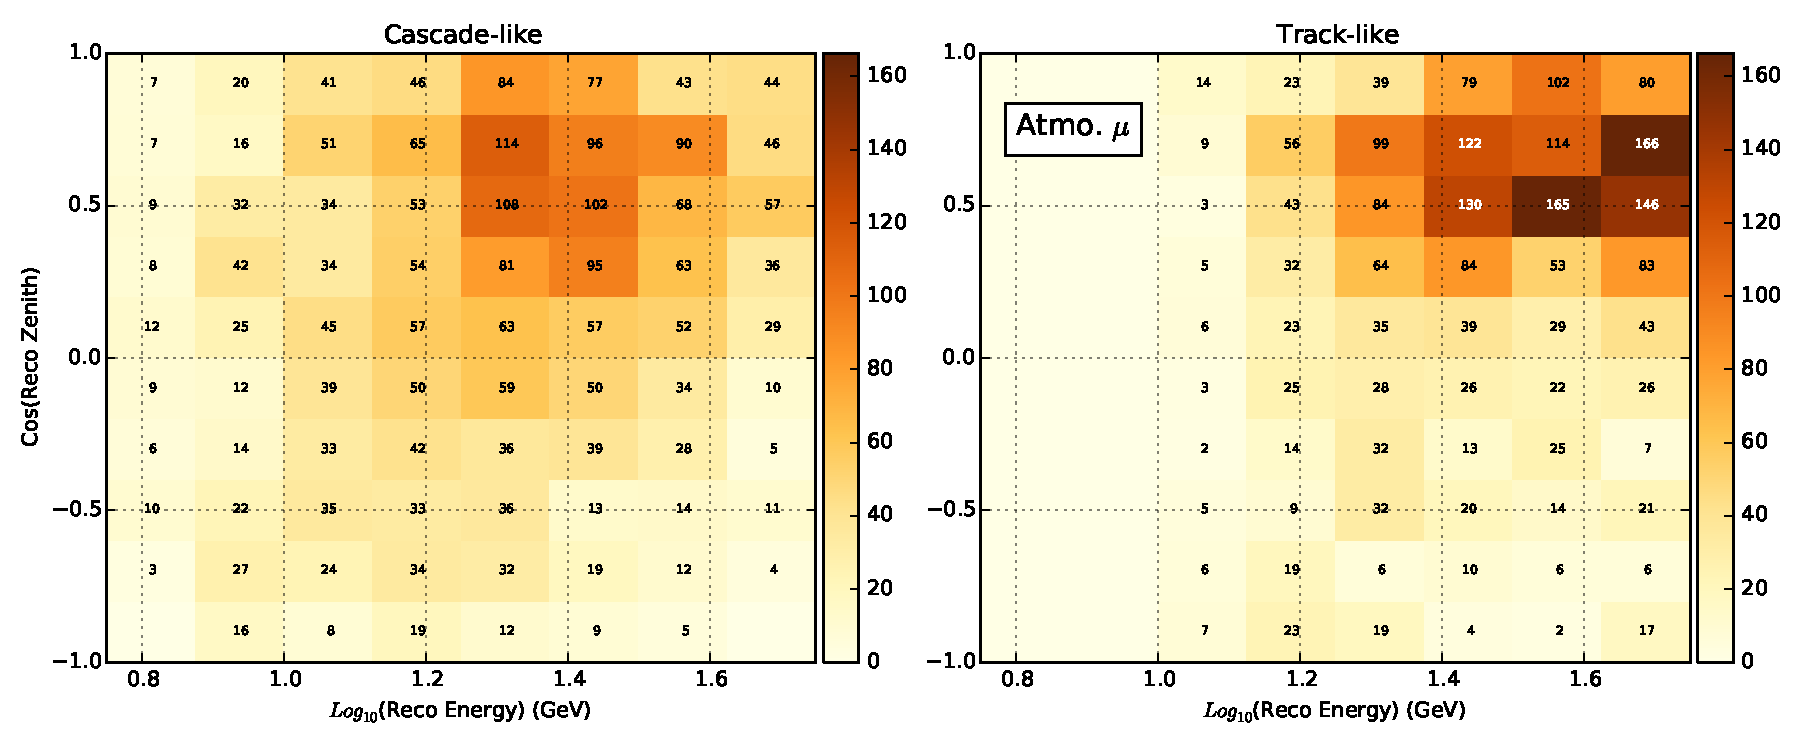
\includegraphics[width=0.7\textwidth]{templates/muongundima.pdf}  \\
  \small (\textbf{\color{ctcolormain}a}) Atmospheric $\mu$
\end{tabular}
\linebreak
\begin{tabular}[b]{c}
  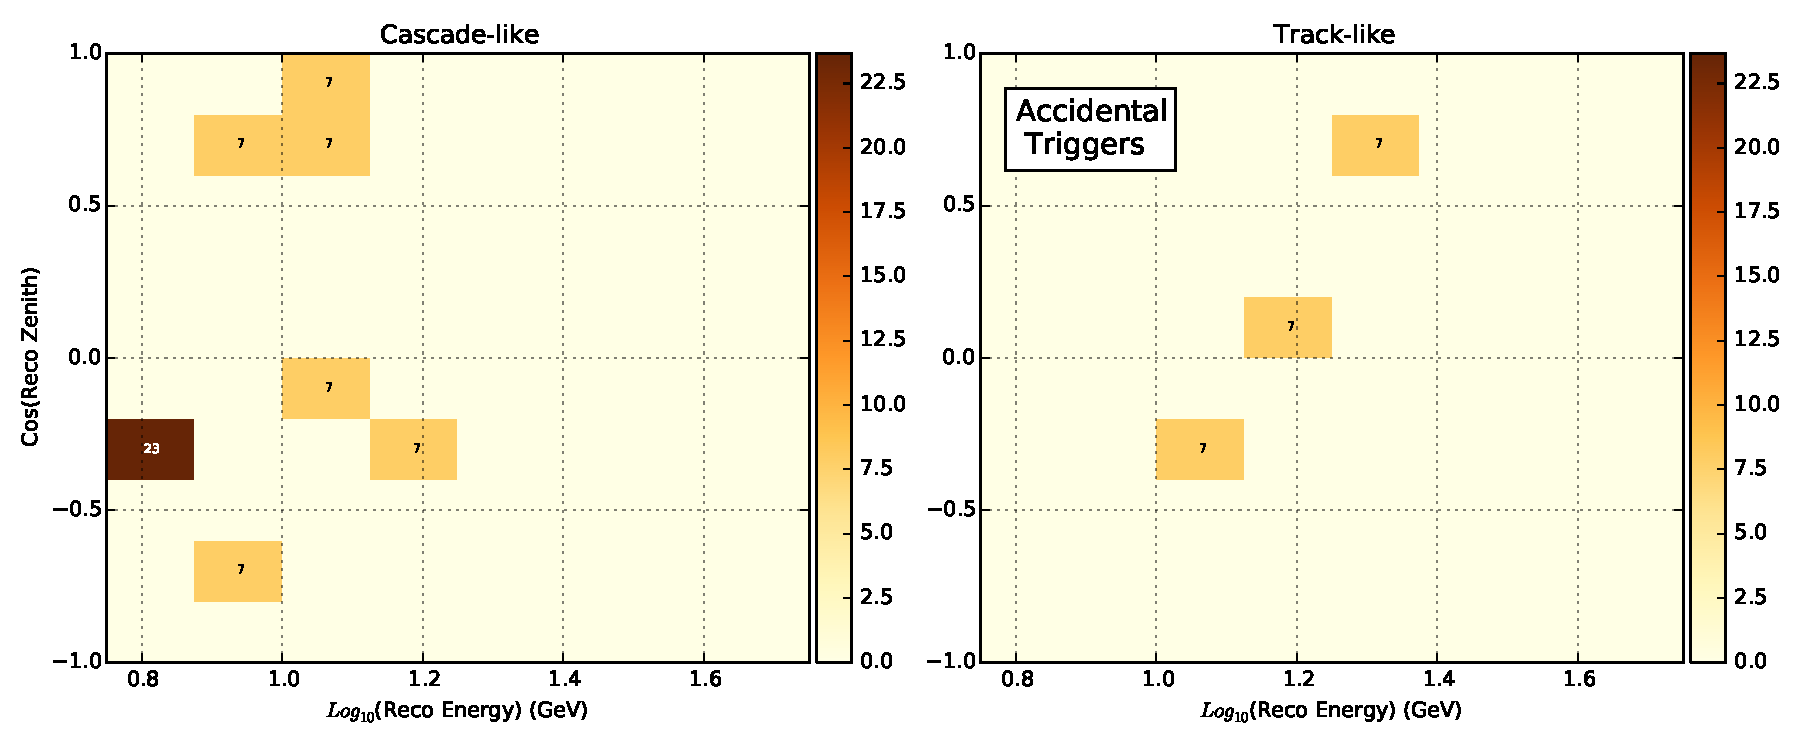
\includegraphics[width=0.7\textwidth]{templates/vuvuzela.pdf}  \\
  \small (\textbf{\color{ctcolormain}b})  Accidental Triggers
\end{tabular}
\linebreak
\begin{tabular}[b]{c}
  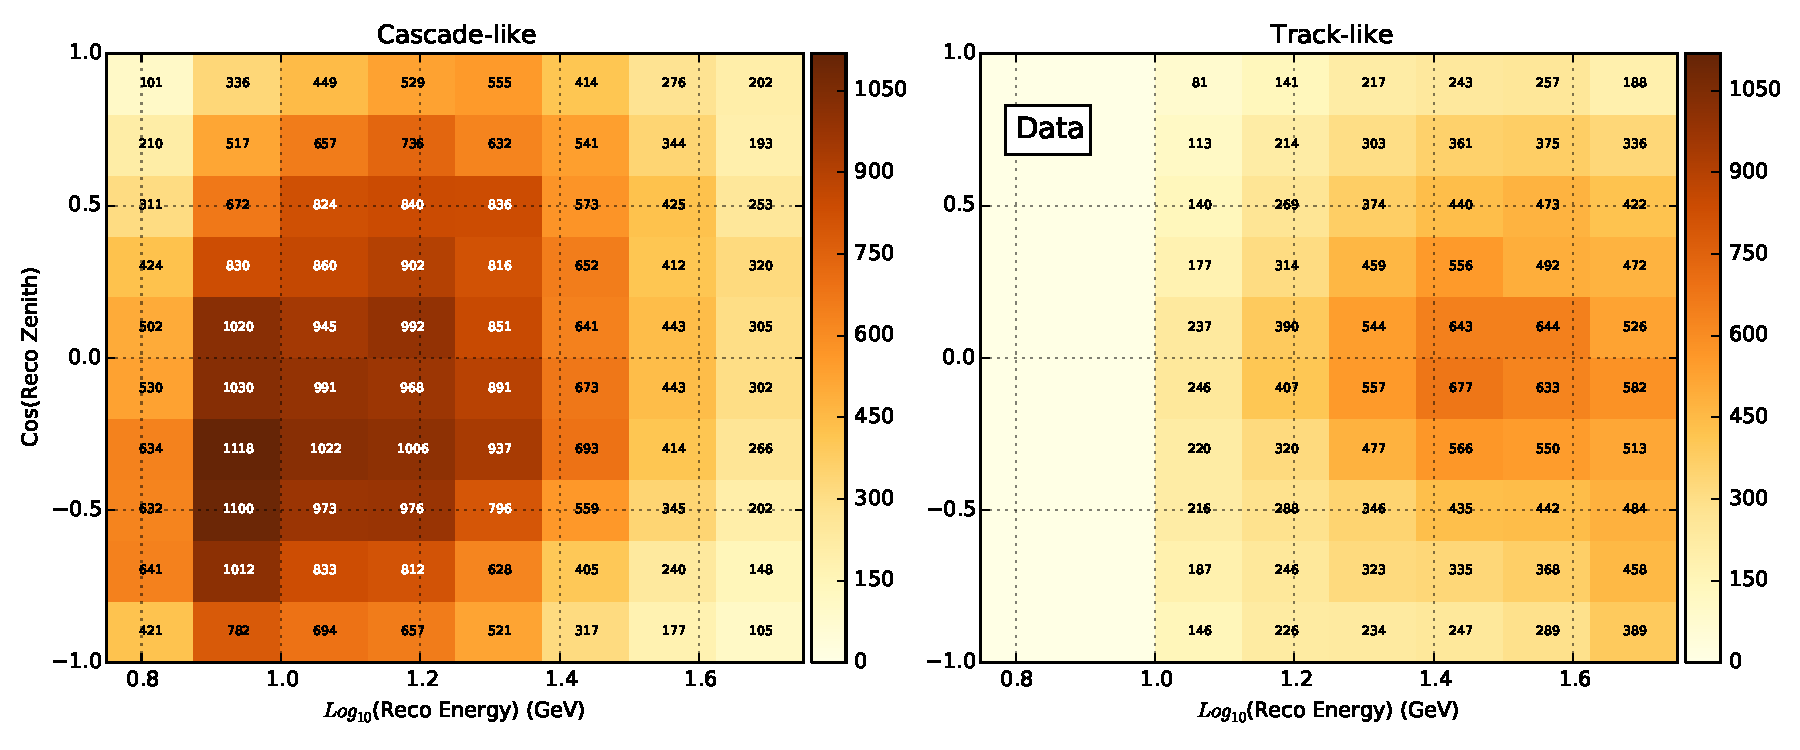
\includegraphics[width=0.7\textwidth]{templates/data2012-4.pdf}  \\
  \small (\textbf{\color{ctcolormain}c})  Data
\end{tabular}
\caption[Background and data histograms for appearance analysis]{The background (a, b) and data (c) histograms used in the fit for appearance. The NuFit oscillation parameters are assumed \cite{NuFit.org}. The colorbar shows the expected rate in each bin from the 3 year sample used in this thesis. The numbers in the bins give the expected rate numerically. The disappearance of muon neutrinos is visible in data histogram in the upgoing ($cos(\theta)$=-1) track-like histogram around an energy of $10^{1.3}$=20~GeV. Both the muon and accidental trigger histograms are limited by the simulations statistics. }
\label{fig:bg_data_templates}
\end{figure}

Figure~\ref{fig:bg_data_templates} includes histograms of both the simulated muons, produced using the DeepCore MuonGun generation scheme developed in Section~\ref{sec:muongun_deepcore}, and the accidental triggers, produced using the Vuvuzela V2 model described in Chapter~\ref{chapter:vuvuzela}.
Both samples are limited by the available simulation statististics.
In the case of the accidental triggers, the severely limited statistics available at the Final Level of the analysis precludes the direct use of the remaining events.
Instead, the accidental trigger simulation is modeled assuming a uniform distribution in energy, zenith, and track length with a total event rate equal to the expected rate from the remaining simulation sample..

The muon background histogram contains approximately 2400 simulated events spread over 140 bins in energy, zenith, and track length.
The atmospheric muon background events reconstruct as downgoing events visible in the track-like channel.
Significant statistical uncertainties in the region of expected appearance limit the reach of the analysis.
While additional simulated statistics would be beneficial, potentially following the scheme introduced in Section~\ref{sec:kde_filtering}, the production of new sets has not been completed due to time constraints.


















\label{sec:parametrization_systematics}
\section{Parametrization of Systematic Uncertainties}
The tau neutrino component of the GRECO selection makes up only 5\% of the expected event rate at Final Level.
The measurement is sensitive to a number of \emph{systematic uncertainties}, including the neutrino oscillation parameters, the neutrino and muon fluxes, neutrino cross sections, and various detector systematic uncertainties.
These uncertainties may be divided into two broad categories related to the method in which they are applied.

The first, the \emph{analytic systematic uncertainties} (\emph{ASU}), have an analytic form that may be used to modify the weight of each event. 
Analytic uncertaintes are calculated as modifications to the energy- and zenith-dependent flux weights of the event, $f(E_i, \theta_i)$ to get the final event weight, $w_i$.

\begin{equation}
	w_i = \left( \prod_{m}^{ASU} \delta w_{im} \right) f(E_i, \theta_i)
\end{equation}

\emph{Non-analytic systematic uncertainties} (\emph{NSU}) require dedicated Monte Carlo simulations to parametrize the effects at Final Level.
Properties which affect the trigger conditions or change the properties of photon propagation are examples of non-analytic uncertainties.
These uncertainties cannot be evaluated at a per-event level and are instead applied as changes to the binned analysis histogram in energy, zenith, and track length.

Parametrizing non-analytic uncertainties requires dedicated simulation sets, known as \emph{systematics sets}, such as those in Tables~\ref{table:geniesets} and \ref{table:mgsets}.
Each systematic set must be processed through the GRECO processing stream and reconstructed with the Pegleg reconstruction.
The histograms associated with each systematic set are compared to the \emph{baseline set} to identify the effects of the systematic uncertainty in the reconstructed histogram.
The systematic sets each provide a discrete point describing the change in the analysis histogram due to the selected non-analytic systematic uncertainty.



\label{subsec:hyperplanes}
\subsection{Parametrizing with Hyperplanes}
For the GRECO tau neutrino appearance, a continuous parametrization of the discrete systematics sets is used to model the uncertainties.
The parametrization method can be described by beginning with a simpler model in one dimension.

A simple linear parametrization of one non-analytic systematic uncertainty in a single bin is a linear model of the form

\begin{equation}
	f^\prime = \left( a(x - x_0) + b\right) f
\end{equation}
%
where $x$ and $x_0$ are the current value and the baseline value of the systematic parameter and $f$ and $f^\prime$ are the expected rate in the bin before and after applying the effect of the systematic uncertainty.
The constants, $a$ and $b$, are fit to the expected rates from the systematic sets $\vec{f}_{SystSets}$ as a function of the systematic values $\vec{x}_{SystSets}$ using the linear least squares method.
This linear model provides a continuous parametrization from the discrete set of points and is used to describe the effect of the systematic parameter in the analysis histogram.

The model can be trivially extended to include multiple systematic uncertainties using a similar form.

\begin{equation}
\label{eq:hyperplane_nu}
	f^\prime = \left( \sum_{m}^{NSU} \left(a_m (x_m - x_{m0})\right) + b\right) f
\end{equation}
%
All systematic effects $m$ are described by independent linear models with a common constant $b$.
The constants [$a_0$, $a_1$, ...] and $b$ are once again fit using the linear least squares method.

This model, referred to as a \emph{hyperplane}, is used to describe the non-analytic systematics for each bin for the neutrinos.
For atmospheric muons, the form is slightly modified to account for large changes in rate due to DOM efficiency and absorption uncertainties.
In these two cases, an exponential model is selected to better describe the observed effects in simulation.

\begin{equation}
\label{eq:hyperplane_mu}
	f^\prime = 
	\left(\sum_{m\neq DE,Abs}^{NSU}\left(a_m (x_m-x_{m0})\right) + \sum_k^{DE,Abs}\left(a_k e^{b_k (x_k-x_{k0})} - 1\right) + c\right) f
\end{equation}

Separate hyperplanes are created for each bin in energy, zenith, and track length as well as for each simulated event type ($\nu^{CC}_e$, $\nu^{CC}_\mu$, $\nu^{CC}_\tau$, $\nu^{NC}$, $\mu$).
These parametrizations allow the evaluation of the effect of any combination of the six non-analytic systematics.


\begin{landscape}
\begin{table}[]
\centering
\begin{tabular}{@{}llllllll@{}}
\toprule
Set Number & Coincident Fraction & DOM Eff & Hole Ice & Forward Coeff & Absorption & Scattering & Processed Livetime \\ \midrule
Baseline  & 0\%                 & 100\%   & 25       & 0             & 100\%      & 100\%      & 30 years \\ \midrule
640C      & 100\%               & 100\%   & 25       & 0             & 100\%      & 100\%      & 30 years \\ \midrule
641        & 0\%                 & 88\%    & 25       & 0             & 100\%      & 100\%      & 30 years \\
643        &                     & 94\%    &          &               &            &            &          \\
644        &                     & 97\%    &          &               &            &            & 10 years         \\
645        &                     & 103\%   &          &               &            &            &          \\
646        &                     & 106\%   &          &               &            &            &          \\
648        &                     & 112\%   &          &               &            &            &          \\ \midrule
660        & 0\%                 & 100\%   & 15       & 0             & 100\%      & 100\%      & 10 years \\
661        &                     &         & 20       &               &            &            &          \\
662        &                     &         & 30       &               &            &            &          \\
663        &                     &         & 35       &               &            &            &          \\ \midrule
670        & 0\%              & 100\%  & 25 & 2.0           & 100\%  & 100\%  & 10 years \\ 
671        &                     &         &          & -5.0          &            &            &         \\
672        &                     &         &          & -3.0          &            &            &          \\
673        &                     &         &          & 1.0           &            &            &          \\
674        &                     &         &          & -1.0          &            &            &          \\ \midrule
681        & 0\%                 & 100\%   & 25       & 0.0           & 92.9\%     & 92.9\%     & 30 years \\
682        &                     &         &          &               & 110\%      & 100\%      &          \\
683        &                     &         &          &               & 100\%      & 110\%      &         
\end{tabular}
\caption[Available systematics simulation sets for GENIE]{Simulation sets used to describe non-analytic uncertainties of the signal neutrino events. The sets are divided into categories in which only one parameter is changed. Only parameters which are varied are shown for each row. While all listed sets have up to 30 years of effective livetime available, not all events are processed in each set due to the computational constraints of the Pegleg reconstruction.}
\label{table:geniesets}
\end{table}
\end{landscape}


\begin{landscape}
\begin{table}[]
\centering
\begin{tabular}{@{}llllllll@{}}
\toprule
Set Number & Oversizing & DOM Eff & Hole Ice & Forward Coeff & Absorption & Scattering & Comments                \\ \midrule
Baseline   & 1.0        & 99\%    & 25       & 0             & 100\%      & 100\%      & 1 year DeepCore MuonGun \\ \midrule
A          & 1.0        & 69.3\%  & 30       & 0             & 100\%      & 100\%      &                         \\
B          &            & 79.2\%  &          &               &            &            &                         \\ \midrule
C          & 1.0        & 99\%    & 15       & 0             & 100\%      & 100\%      &                         \\
D          &            &         & 30       &               &            &            &                         \\ \midrule
E          & 1.0        & 99\%    & 30       & -2            & 100\%      & 100\%      &                         \\
F          &            &         &          & -4            &            &            &                         \\ \midrule
G          & 3.0        & 99\%    & 25       & 0             & 100\%      & 100\%      & 1 year KDE Prescale     \\
H          &            &         &          &               & 110\%      &            &                         \\
I          &            &         &          &               & 80\%       &            &                         \\
J          &            &         &          &               & 100\%      & 80\%       &                         \\
K          &            &         &          &               &            & 110\%      &                         \\
L          &            &         &          &               &            & 120\%      &                         \\
M          &            &         &          &               & 92.9\%     & 92.9\%     &                         \\
N          &            &         &          &               & 114.2\%    & 114.2\%    &                         \\ \bottomrule
\end{tabular}
\caption[Available systematics sets for MuonGun]{Simulation sets used to describe non-analytic uncertainties of the atmospheric muon events. The sets are divided into categories in which only one parameter is changed. Only parameters which are varied are shown for each row. Note that the bulk ice systematics sets use the KDE prescale simulation scheme introduced in Section~\ref{sec:kde_filtering}.}
\label{table:mgsets}
\end{table}
\end{landscape}












\label{sec:systematics}
\section{Effects of Systematic Uncertainties}
A set of 18 systematic uncertainties were used in the search for tau neutrino appearance.
These parameters consist of the muon neutrino disappearance parameters as well as uncertainties in the flux, the cross sections, and the detector modeling.
Each systematic will be briefly discussed and the effect on the analysis histogram will be shown.


\label{subsec:oscillation_params}
\subsection{Oscillation Parameters}
The GRECO selection is sensitive to atmospheric neutrinos from 5 GeV to 60 GeV with a peak energy around 20 GeV.
These neutrinos travel distances from approximately 20 km (directly downgoing) to 12700 km (directly upgoing), giving a range of 0.35~$\leq$~L/E~$\leq$~2540.
At these energies and baselines, the solar mass splitting $\Delta m^2_{21}=7.49\times 10^{-5} eV^2$ is too small to be important.
This also limits the sensitivity of the GRECO events to the solar mixing angle $\theta_{12}$.

Only the atmospheric parameters, $\Delta m^2_{31}$ and $\theta_{23}$, and the reactor angle, $\theta_{13}$ may contribute.
The reactor mixing angle affects the oscillation probability to electron neutrinos through the MSW effect at the GeV scale.
Measurement contraints on $\theta_{13}$ limit the uncertainty on this parameter.

This has been tested with the GRECO sample by changing each parameter by the 1${\sigma}$ range given in \cite{NuFit.org}.
The total value of the ${\chi^2}$, defined as in Section~\ref{subsec:chi2}, was used to select the most important parameters for this fit.

\begin{table}[]
\centering
\begin{tabular}{@{}llll@{}}
\toprule
Parameter                & Baseline                                         & Tested Shift                                   & $\sum_{bins}\chi^2$                     \\ \midrule
$\Delta m^2_{31}$ & 2.2526${\times 10^{-3}}$ & +0.10 ${\times 10^{-3}}$  & 2.776                                             \\
$\Delta m^2_{21}$ & 7.49 ${\times 10^{-5}}$    & +0.19 ${\times 10^{-5}}$  & 5.392  ${\times 10^{-4}}$  \\
$\theta_{23}$        & 0.72431                                        & +0.02094                                       & 1.262                                             \\
$\theta_{13}$        & 0.14765                                        & +0.00262                                       & 1.802 ${\times 10^{-3}}$   \\
$\theta_{12}$        & 0.58853                                        & +0.01379                                       & 2.978 ${\times 10^{-4}}$   \\ 
$\delta_{CP}$         & 0.0                                                & +$\frac{\pi}{2}$                             & 2.407 ${\times 10^{-2}}$    \\ \bottomrule
\end{tabular}
\caption[Total $\chi^2$ impact of each of the oscillation parameters]{Total $\chi^2$ impact of each of the oscillation parameters. A $\sum\chi^2~\approx~1$ corresponds to a 1$\sigma$ effect in the histogram. The atmospheric mixing parameters, $\Delta m^2_{31}$ and $\theta_{23}$ are the most important oscillation parameters for the GRECO selection. Of the remaining parameters, the CP-violating phase is the next most imporant. }
\label{tab:oscil_impact}
\end{table}

The results are shown in Table~\ref{tab:oscil_impact}.
The atmospheric mixing parameters, $\Delta m^2_{31}$ and $\theta_{23}$, have significantly larger impacts on the analysis histogram than the other parameters.
For the purposes of GRECO analyses, only these parameters are therefore considered.

The effect of each is shown in Figures~\ref{fig:systematics_dm31} and \ref{fig:systematics_theta23}.
Of the two, the mass splitting term has strong correlations expected with tau neutrino normalization $N_{\nu_\tau}$, changing both the location as well as the strength of the observed appearance.

The track-like and cascade-like histograms are both dominated by muon neutrino charged current interactions.
Both the track-like and cascade-like events see strong effects from the uncertainties on the atmospheric mixing parameters.


\begin{figure}
\centering
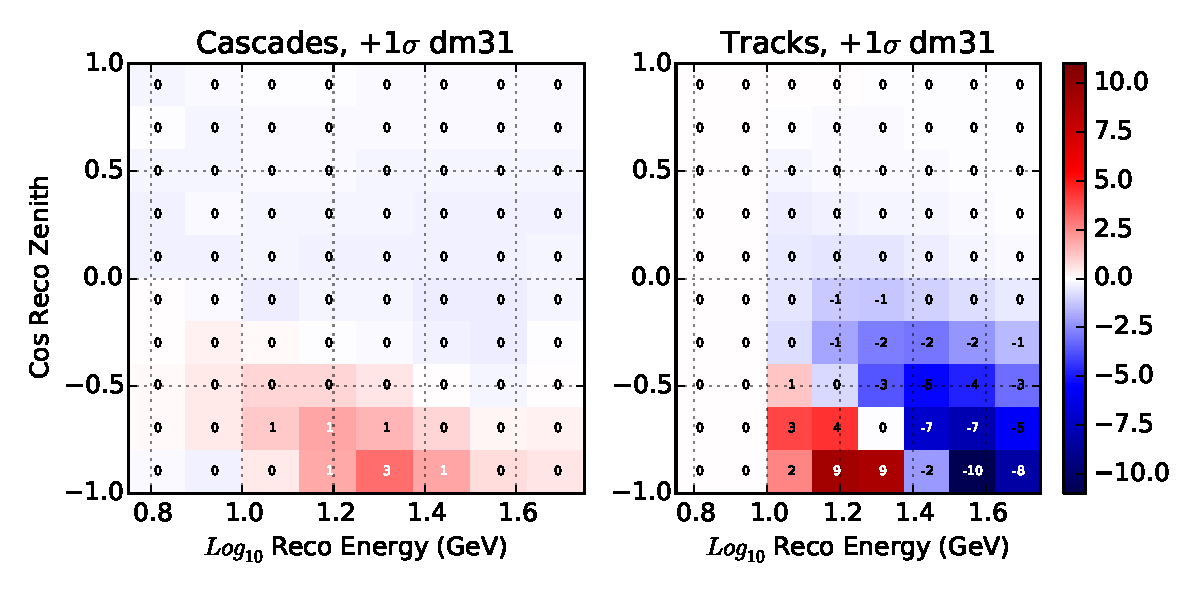
\includegraphics[width=0.9\textwidth]{systematics/dm31_variation.pdf} 
\caption[Effect of $\Delta m^2_{31}$ in the analysis histogram]{The effect of $\Delta m^2_{31}$ in the analysis histogram. The colorbar shows the percent change in rate per bin for a shift of 10\% in the mass splitting from the baseline value, 2.526 $\cdot 10^{-3}~eV^2$, to 2.779 $\cdot 10^{-3}~eV^2$. A strong disappearance effect is observed in the track-like events while the number of events in the appearance signal region of the cascade-like histogram is increased. Of the systematic uncertainties included in the tau neutrino appearance analysis, the mass splitting shows the strongest correlation with the value of $N_{\nu_\tau}$.}
\label{fig:systematics_dm31}
\end{figure}

\begin{figure}
\centering
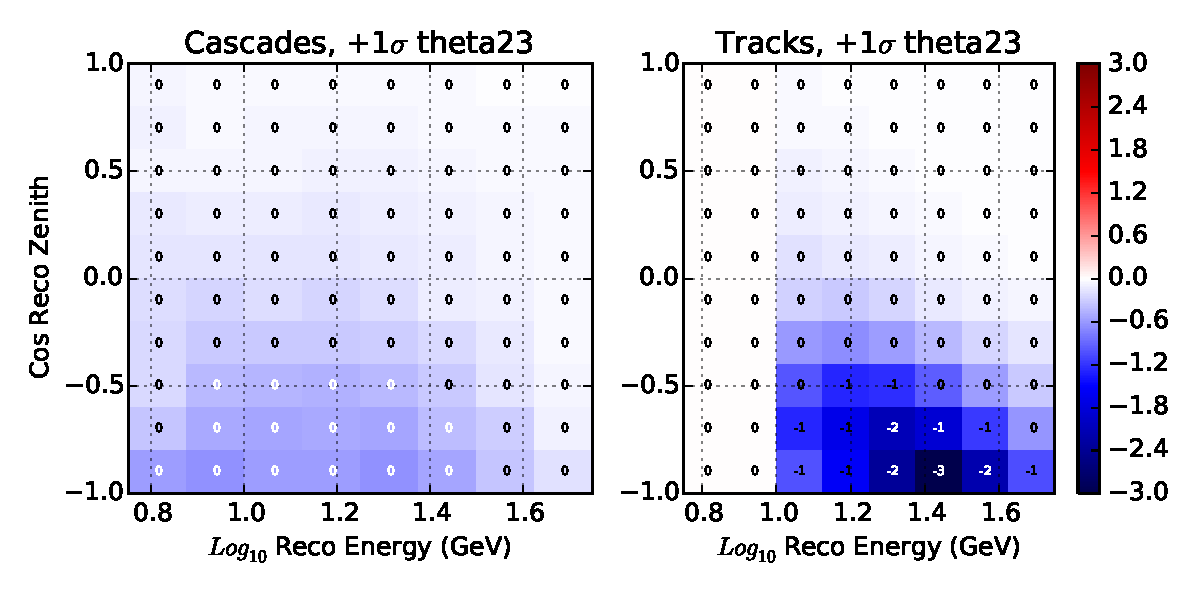
\includegraphics[width=0.9\textwidth]{systematics/theta23_variation.pdf} 
\caption[Effect of $\theta{23}$ in the analysis histogram]{The effect of $\theta_{23}$ in the analysis histogram. The colorbar shows the percent change in rate per bin for a shift of 10\% from the baseline value, $sin^2\theta_{23}=0.440$, to $sin^2\theta_{23}=0.50$. As expected, the appearance modulates the strength of the muon neutrino disappearance. Because both the cascade-like and track-like sample are dominated by muon neutrino charged current events, this change results in a net disappearance in both histograms.}
\label{fig:systematics_theta23}
\end{figure}



\label{subsec:nuflux_systematics}
\subsection{Neutrino Flux Uncertainties}
The underlying flux models of the atmospheric neutrinos and background muons contain significant uncertainties relevent to the search for tau neutrino appearance. 
The implementation of the flux used in IceCube is produced using a computationally expensive Monte Carlo simulation of the Earth \cite{Honda-2015}.
Four analytic systematic uncertainties used in this analysis modify the neutrinos flux.
A fifth systematic uncertainty scales the total neutrino flux to account for uncertainties in the total event rate.
This neutrino normalization is allowed to float freely with a constraint that the value be larger than 0.

\label{subsubsec:gamma_nu}
\subsubsection{Neutrino Spectral Index}
\begin{figure}
\centering
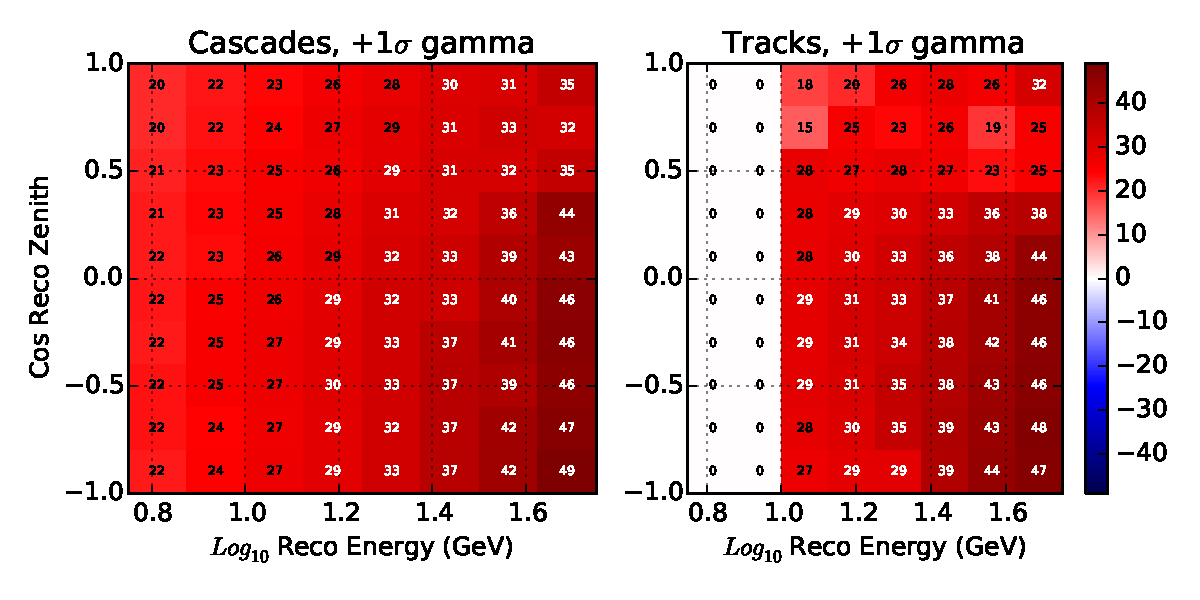
\includegraphics[width=0.9\textwidth]{systematics/gamma_variation.pdf} 
\caption[Effect of $\delta \gamma_\nu$ in the analysis histogram]{The effect of $\delta \gamma_\nu$ in the analysis histogram. The colorbar shows the percent change in rate per bin for a shift of 10\% from the baseline value. The spectral index has a strong effect on both histograms as a function of energy.}
\label{fig:systematics_gamma}
\end{figure}

The spectral index of the neutrino flux is related to the cosmic ray spectrum. 
The change in the neutrino flux, $\delta \gamma_\nu$ is implemented by modifying the neutrino event weight, $w_i$ based on the energy of the event.

\begin{equation}
w'_i = \left(\frac{E_{i}}{1~GeV}\right)^{\delta \gamma_\nu} w_i
\end{equation}

For IceCube, a gaussian prior of 0~$\pm$~0.1 is used for the uncertainty in the spectral index.
The effect is shown in Figure~\ref{fig:systematics_gamma}.


\label{subsubsec:nue_ratio}
\subsubsection{$\nu_e/\nu_\mu$ Ratio}
\begin{figure}
\centering
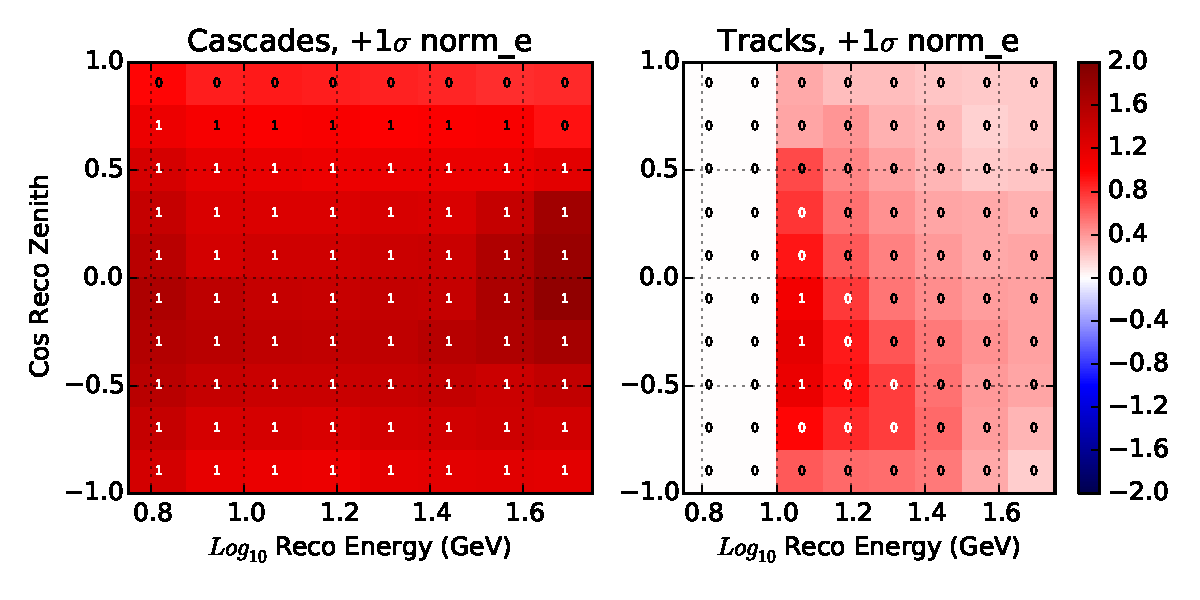
\includegraphics[width=0.9\textwidth]{systematics/norm_e_variation.pdf} 
\caption[Effect of $N_{\nu_e}$ in the analysis histogram]{The effect of $N_{\nu_e}$ in the analysis histogram. The colorbar shows the percent change in rate per bin for a shift of 5\% from the baseline value. The strongest impact occurs in the cascade-like events near the horizon.}
\label{fig:systematics_norm_e}
\end{figure}

The number of electron and muon neutrinos produced during air showers depends on the dynamics of the shower and the hadronization model used in the prediction.
For IceCube, the ratio of the electron and muon fluxes is used as a systematic by scaling the normalization of the two fluxes.
The scaling factor, $N_{\nu_e}$ is applied to the electron neutrino flux as a flat scale factor with a conservative prior of 1.0~$\pm$~0.05 derived from \cite{NuFlux-Barr}.
The effect on the histogram is shown in Figure~\ref{fig:systematics_norm_e}.


\label{subsubsec:barr_ratios}
\subsubsection{$\nu/\bar{\nu}$ and Upward/Horizontal Ratios}
\begin{figure}
\centering
\begin{tabular}[b]{c}
  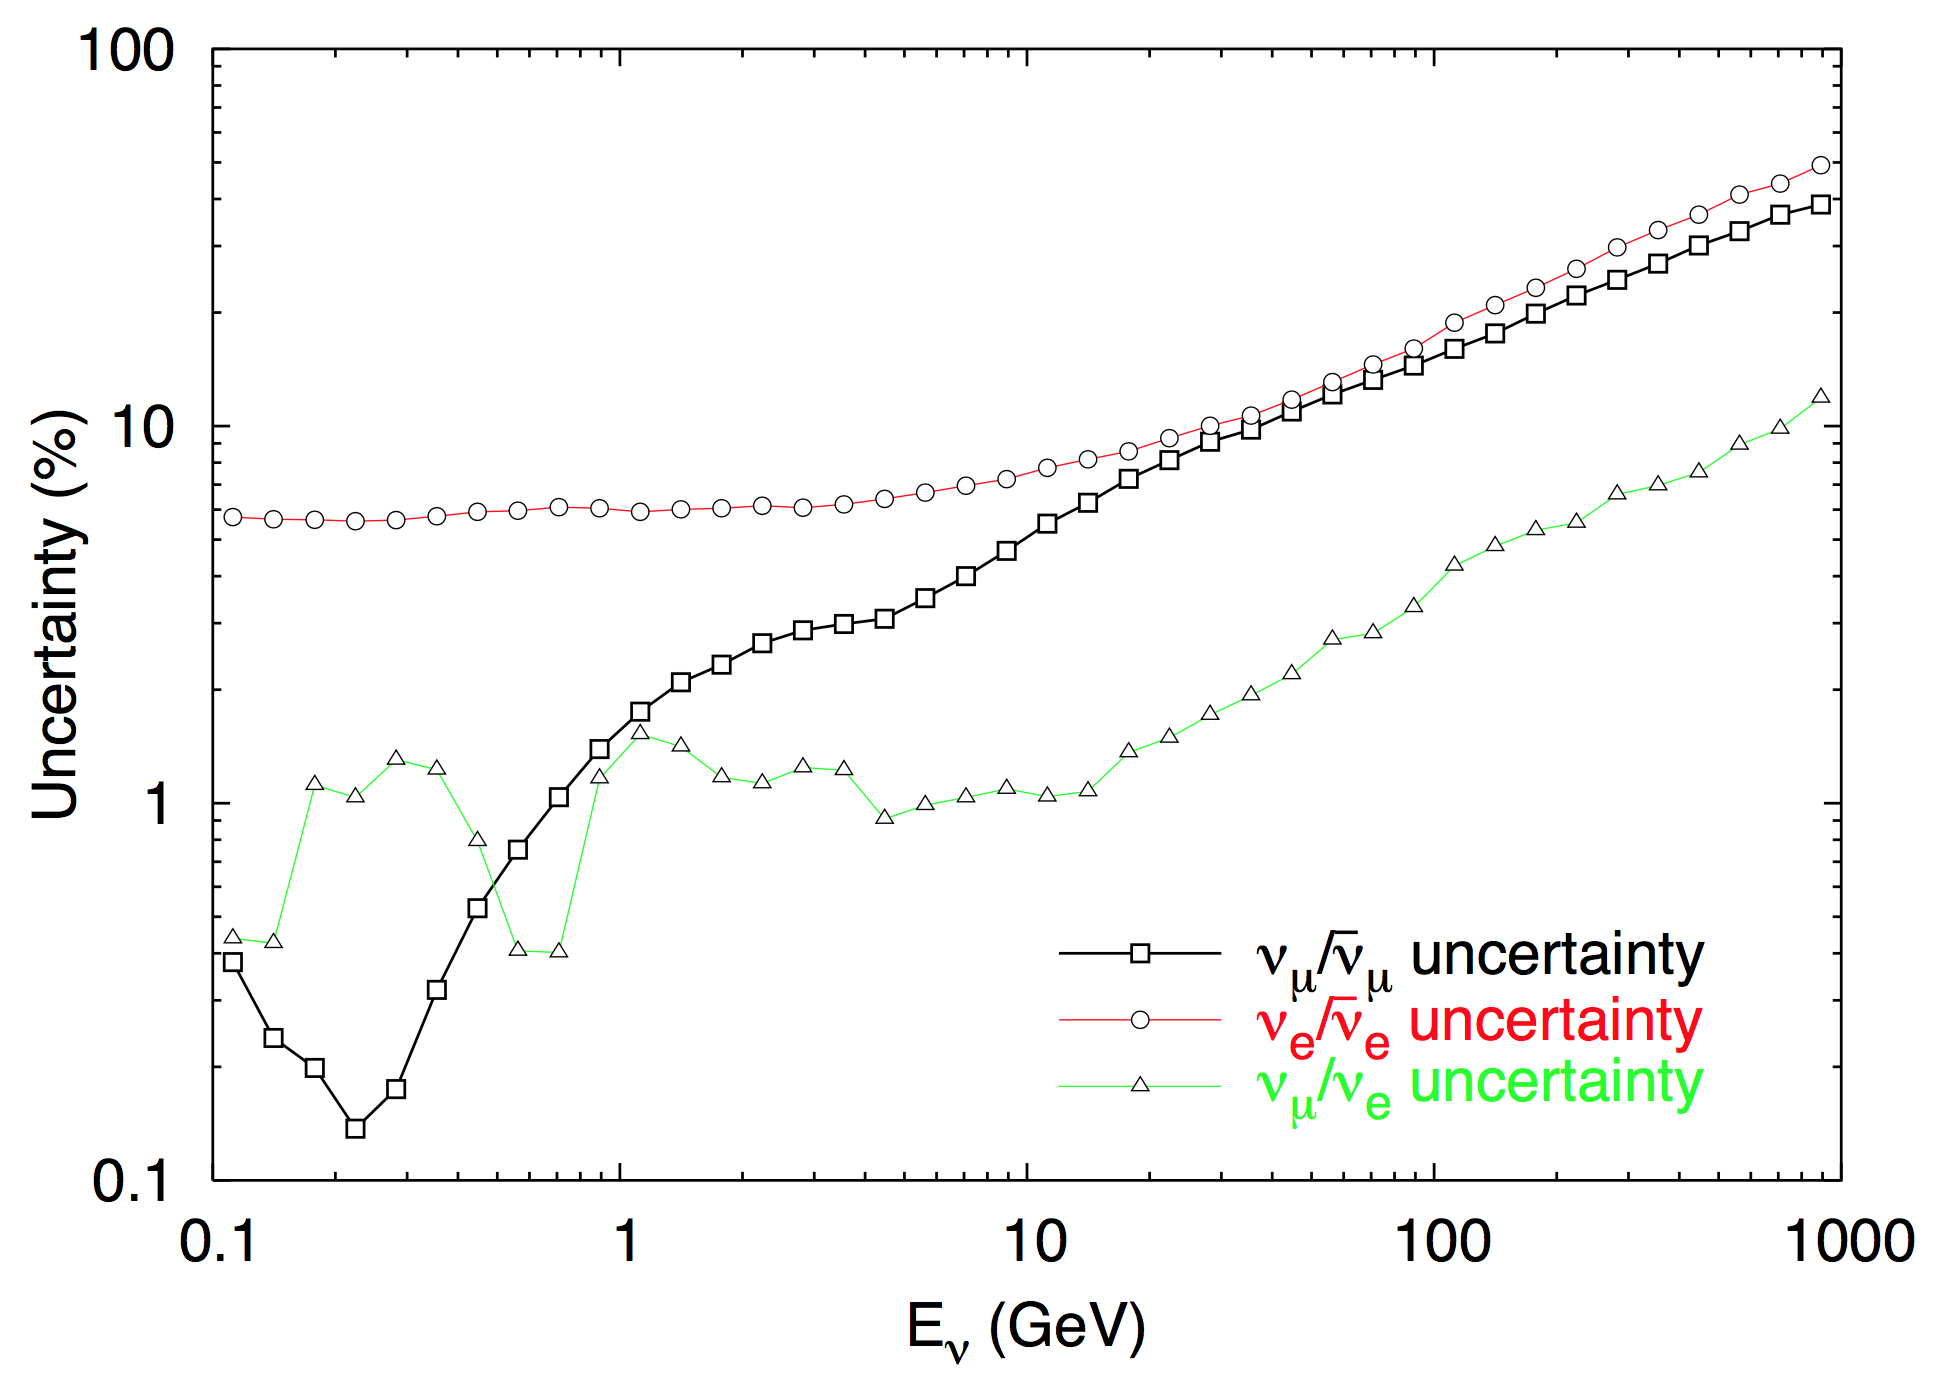
\includegraphics[width=0.45\linewidth]{systematics/barr_nunubar.png} \\
  \small (\textbf{\color{ctcolormain}a}) $\nu/\bar{\nu}$ Uncertainties
\end{tabular} \hspace{2pt}
\begin{tabular}[b]{c}
  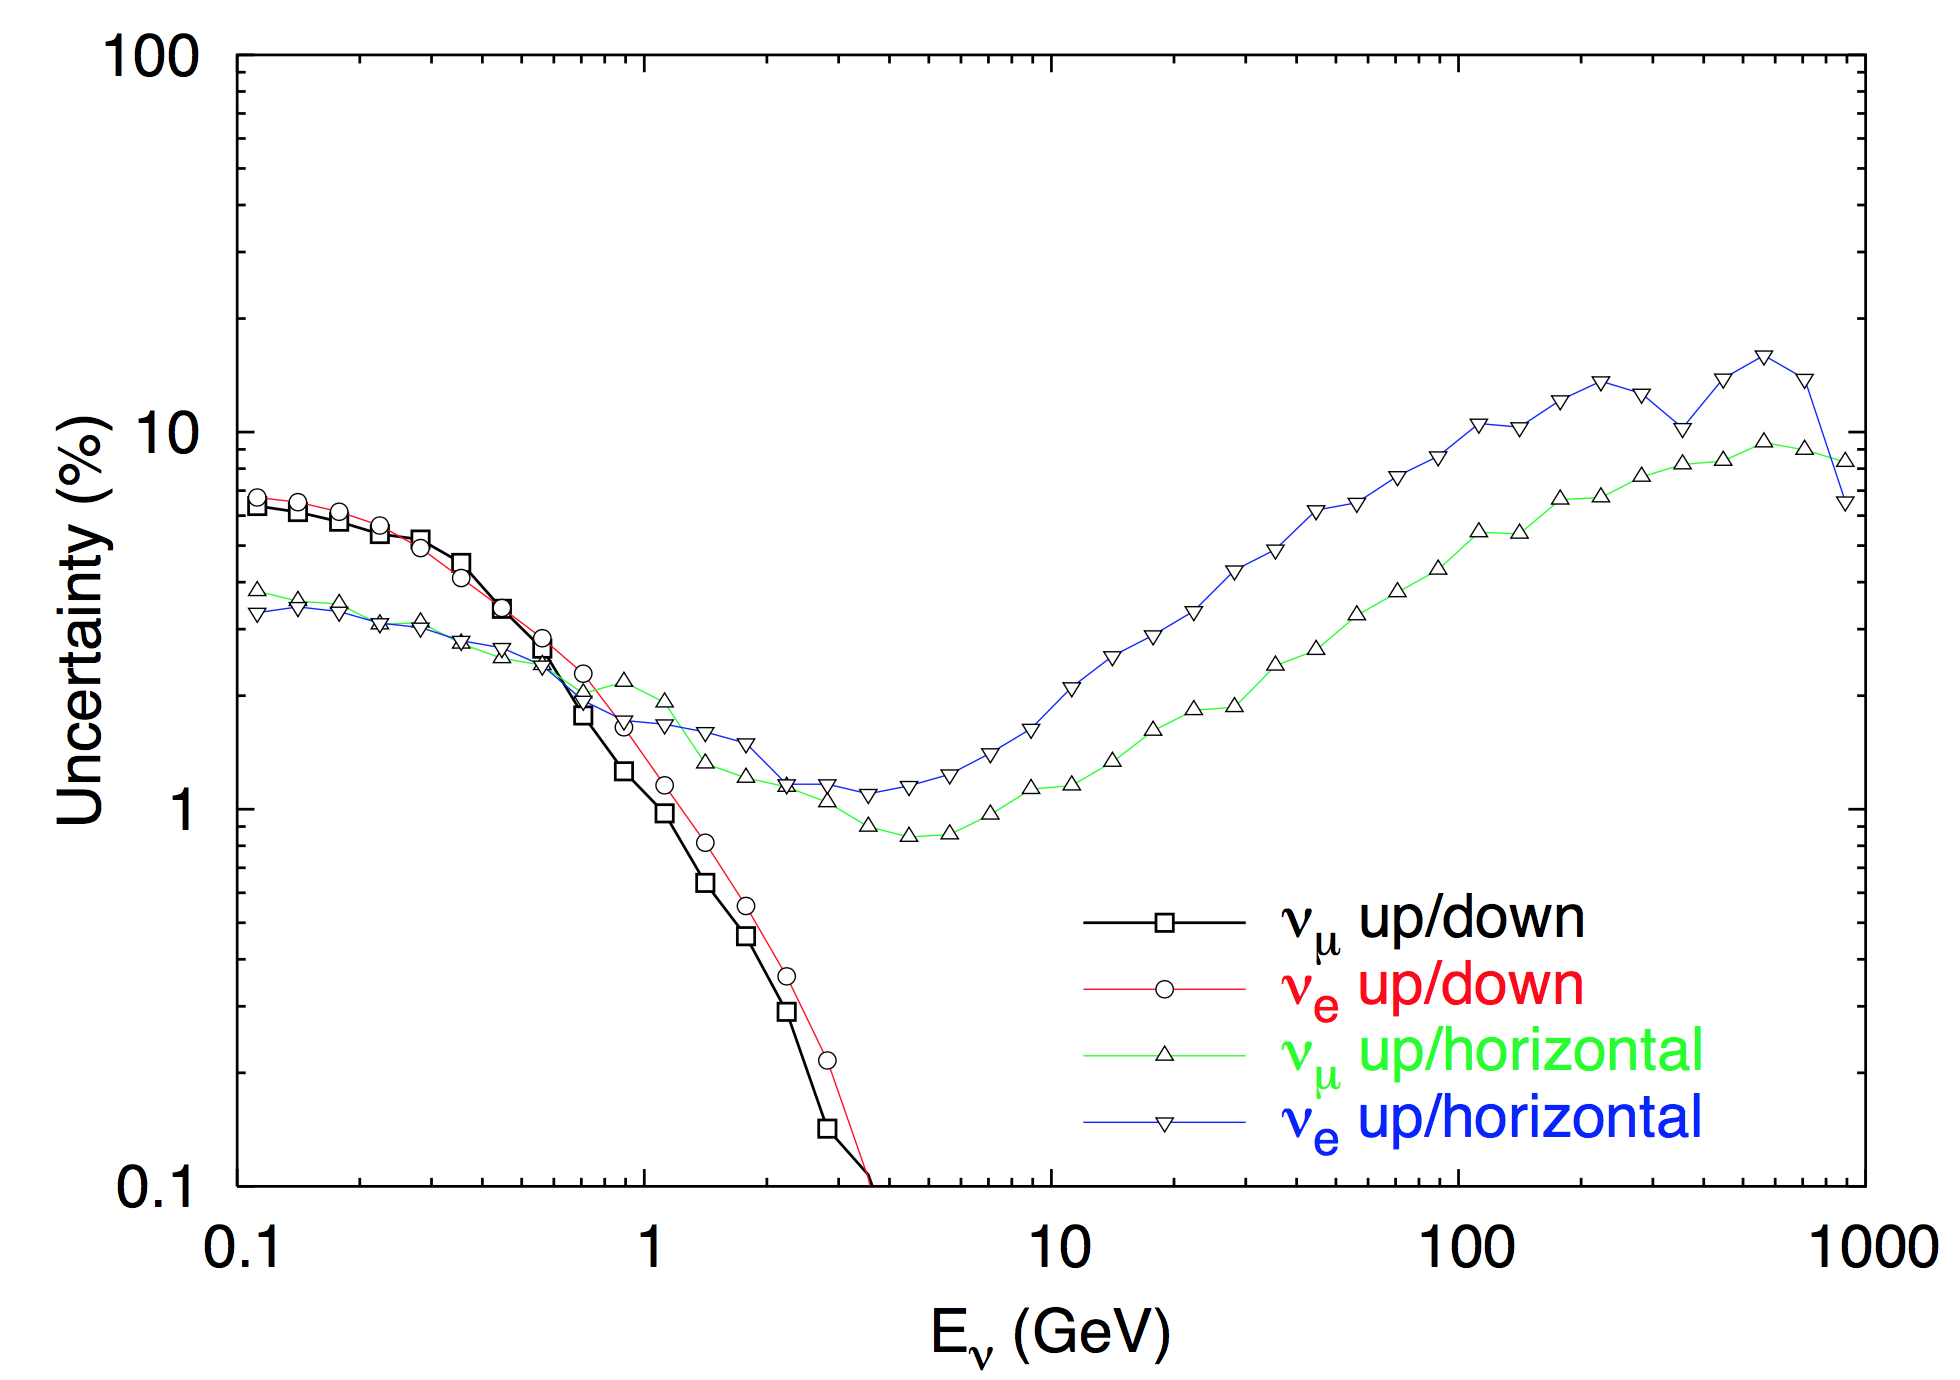
\includegraphics[width=0.45\linewidth]{systematics/barr_uphor.png} \\
  \small (\textbf{\color{ctcolormain}b}) Upward/Horizontal Uncertainties
\end{tabular}
\caption[The neutrino flux shape uncertainties]{The neutrino flux uncertainties calculated in \cite{NuFlux-Barr}. (a) The ratio of the  muon to electron neutrino fluxes is shown in green. The effect is applied as an energy-independent scale factor with a conservative prior of 5\% adopted in this analysis. The uncertainty of the neutrino to antineutrino flux, shown in black and red for muon neutrinos and electron neutrinos respectively, is parametrized as a function of energy and zenith for inclusion in the appearance analysis. (b) The ratio of the upward flux to the horizontal flux in the atmospheric neutrinos. The ratio changes due to uncertainties in the pion and kaon decays in cosmic ray air showers. The shape of the uncertainty is parametrized in energy and zenith for inclusion in this analysis.}
\label{fig:barr_uncertainties}
\end{figure}

\begin{figure}
\centering
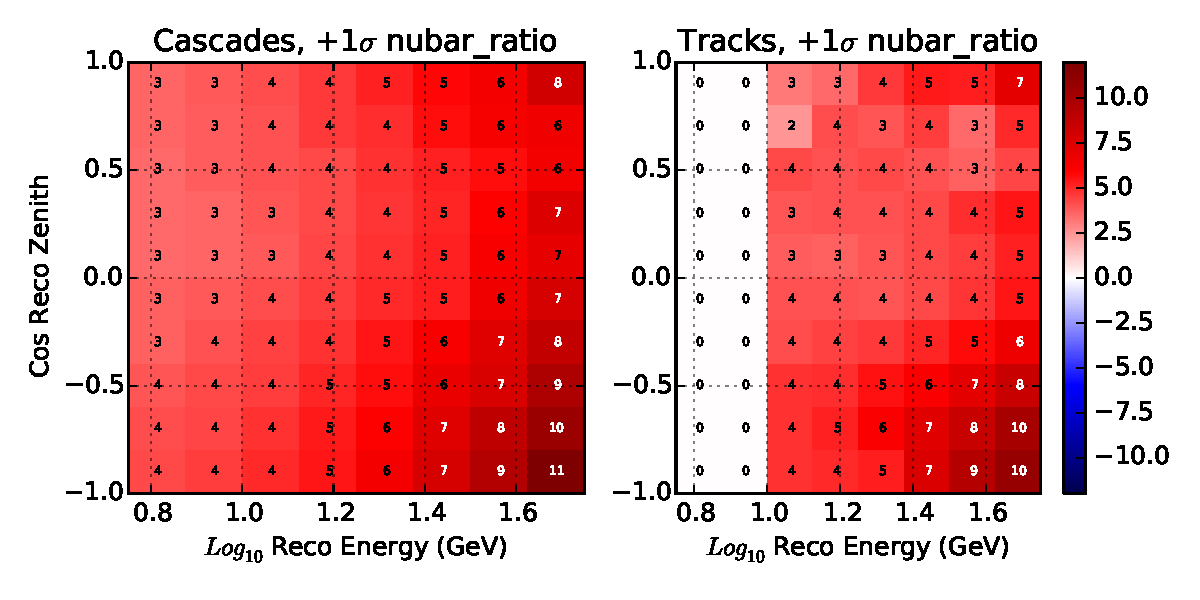
\includegraphics[width=0.9\textwidth]{systematics/nubar_ratio_variation.pdf} 
\caption[Effect of $\nu/\bar{\nu}$ in the analysis histogram]{The effect of the $\nu/\bar{\nu}$ uncertainty in the analysis histogram. The colorbar shows the percent change in rate per bin for a shift of 1$\sigma$ from the baseline value where 1$\sigma$ corresponds to the uncertainties of Figure~\ref{fig:barr_uncertainties}a. Changing the ratio affects both histograms with the strongest effect occuring at the highest energies as expected from \cite{NuFlux-Barr}.}
\label{fig:systematics_nubar_ratio}
\end{figure}

\begin{figure}
\centering
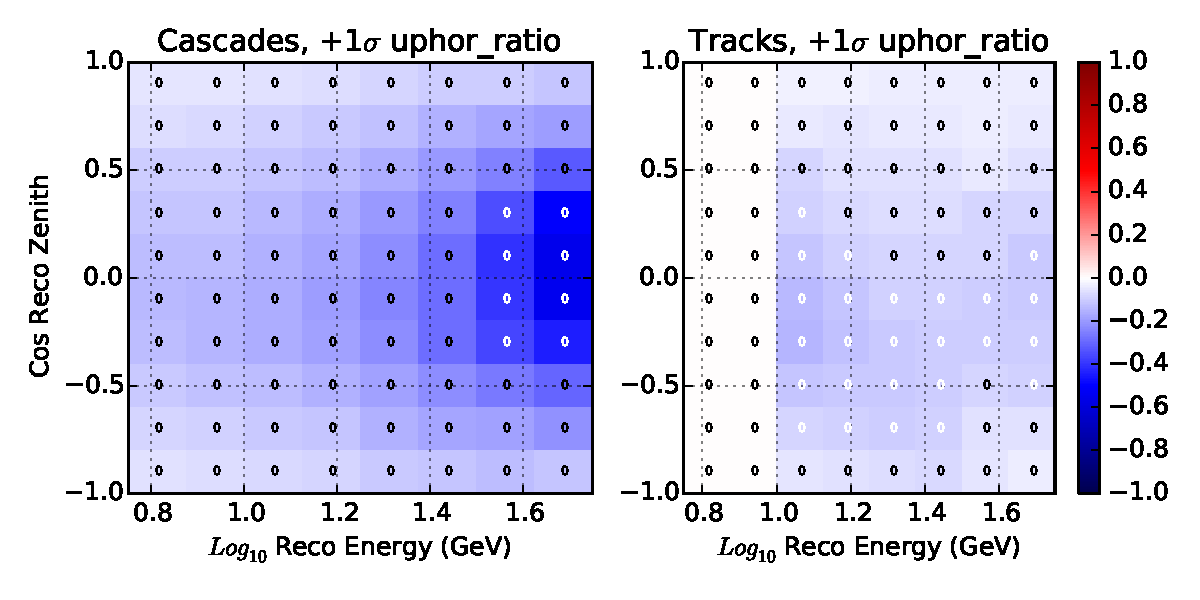
\includegraphics[width=0.9\textwidth]{systematics/uphor_ratio_variation.pdf} 
\caption[Effect of Up/Horizontal in the analysis histogram]{The effect of the upward/horizontal uncertainty in the analysis histogram. The colorbar shows the percent change in rate per bin for a shift of 1$\sigma$ from the baseline value where 1$\sigma$ corresponds to the uncertainties of Figure~\ref{fig:barr_uncertainties}b. The uncertainty of the up/horizontal ratio has a small impact in the analysis space.}
\label{fig:systematics_uphor_ratio}
\end{figure}

The shape of the neutrino spectrum is derived from Monte Carlo simulations that modify the kaon and pion branching ratios used to calculate the neutrino flux prediction \cite{NuFlux-Barr,NuFlux-Manchester}.
In order to utilize these uncertainties in the appearance analysis, parametrizations of the effects, shown in Figure~\ref{fig:barr_uncertainties}, are included in the analysis \cite{IceCube-Oscillation2015,IceCube-Oscillation2018}.
The effects of the $\nu/\bar{\nu}$ uncertainty and the upward/horizontal uncertainty are shown in Figures~\ref{fig:systematics_nubar_ratio} and \ref{fig:systematics_uphor_ratio} respectively.


\label{subsec:muon_systematics}
\subsection{Atmospheric Muon Flux}
The appearance analysis includes two systematics on the atmospheric muon flux.
The first is a normalization factor that scales the total number muons in the detector.
This normalization is constrained to be positive, but otherwise includes a flat prior.

\begin{figure}
\centering
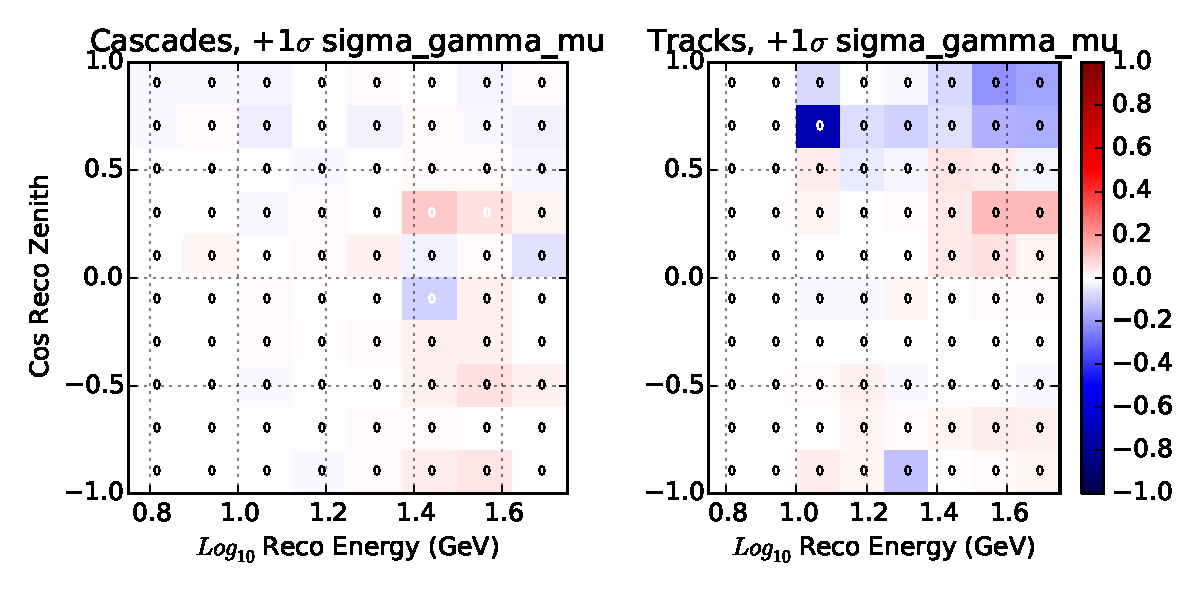
\includegraphics[width=0.9\textwidth]{systematics/sigma_gamma_mu_variation.pdf} 
\caption[Effect of $\delta \gamma_{CR}$ in the analysis histogram]{The effect of the  $\delta \gamma_{CR}$ uncertainty in the analysis histogram. The colorbar shows the percent change in rate per bin for a shift of 1$\sigma$ from the baseline value where 1$\sigma$ corresponds to the uncertainties of \cite{Thesis-Ste}. }
\label{fig:systematics_gamma_mu}
\end{figure}

The second is an uncertainty on the cosmic ray spectral index, $\gamma^{p}_\mu=\2.71\pm~0.01$ for hydrogen nuclei and $\gamma^{He}_\mu=\2.60\pm~0.01$ for helium nuclei, derived from \cite{NuFlux-Manchester}.
The uncertainty was evaluated by reweighting events based on the cosmic ray primary energies of CORSIKA simulation processed to GRECO Level 5.
The resulting uncertainties were parametrized in terms of the energy at the MuonGun generation cylinder (see Section~\ref{sec:muongun_deepcore}) and the direction of the muon \cite{Thesis-Ste}.

The change in the analysis histograms due to the uncertainty in the spectral index of the cosmic ray spectrum is shown in Figure~\ref{fig:systematics_gamma_mu}.
The effect is small, resulting in less than a 0.1\% shift in most bins. 
Despite the small effect, the parameter is included in the fit in order to account for uncertainties in the cosmic ray muons.


\label{subsec:xsec_systematics}
\subsection{Cross-section Uncertainties}
Uncertainties on the neutrino cross section can affect the rates of events in the final sample.
Parametrizations of the QE, RES, and DIS interaction cross section uncertainties were were tested for inclusion in this analysis.

\label{subsubsec:axial_masses}
\subsubsection{Axial Masses}
The axial mass terms, described briefly in Section~\ref{subsec:interactions}, control the cross section for the resonant and quasielastic interactions.
Uncertainties are defined conservatively, following the default uncertainties available in the GENIE generator \cite{GENIE}.

The GENIE generator provides tools to recalculate event weights for changes in the axial masses.
The axial masses and their uncertainties from GENIE are $M_a^{QE}=0.99^{+0.25}_{-0.15}$~GeV and $M_a^{RES}=(1.12 \pm 0.22)$~GeV.

For each QE and RES event, GENIE functions are used to find reweighting factors for 5 discrete points of the axial masses (-2$\sigma$, -1$\sigma$, 0, +1$\sigma$, +2$\sigma$).
These weights are fit to a second order polynomial for each event to produce a smooth parametrization for the weight as a function of axial mass value.

The QE and RES events occur at low energies, as expected from Figure~\ref{fig:xsec}.
The uncertainties reflect this, with the largest impact occuring at low reconstructed energy, as shown in Figures~\ref{fig:systematics_axial_qe} and ~\ref{fig:systematics_axial_res}.


\begin{figure}
\centering
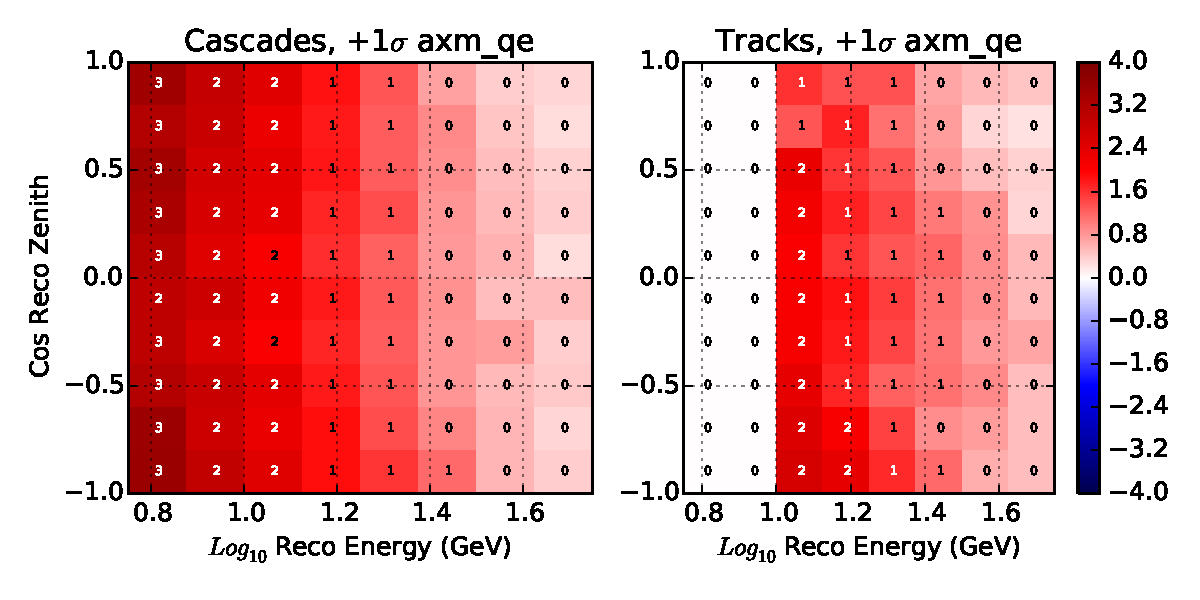
\includegraphics[width=0.9\textwidth]{systematics/axm_qe_variation.pdf} 
\caption[Effect of $M_a^{QE}$ in the analysis histogram]{The effect of the axial mass $M_a^{QE}$ uncertainty in the analysis histogram. The colorbar shows the percent change in rate per bin for a shift of 1$\sigma$ from the baseline value using the GENIE reweighting code.}
\label{fig:systematics_axial_qe}
\end{figure}

\begin{figure}
\centering
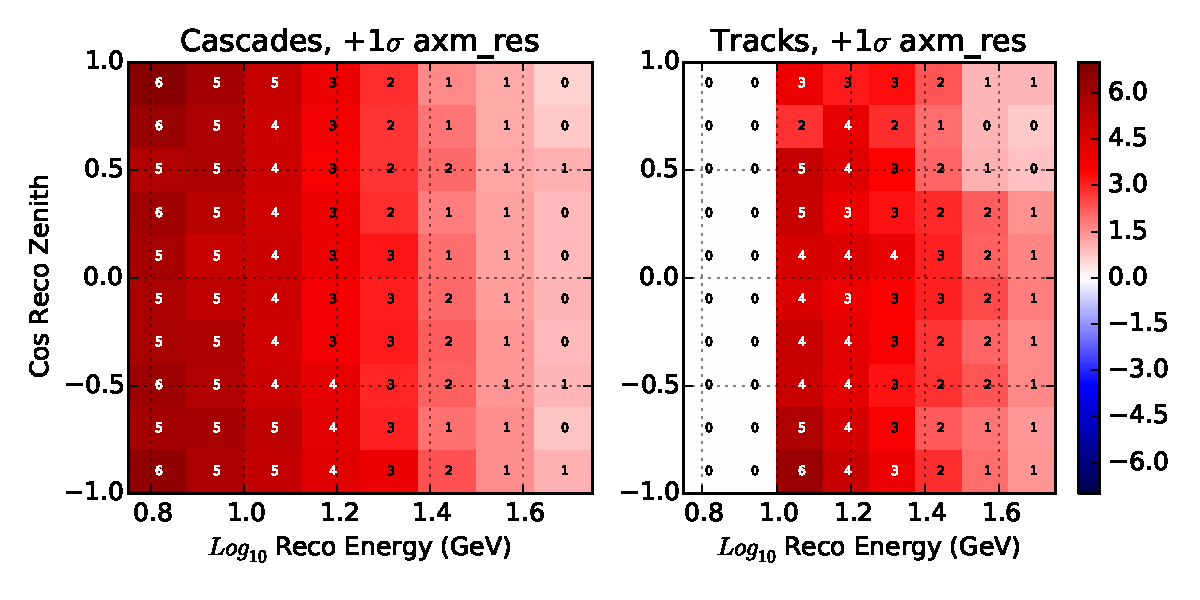
\includegraphics[width=0.9\textwidth]{systematics/axm_res_variation.pdf} 
\caption[Effect of $M_a^{RES}$ in the analysis histogram]{The effect of the axial mass $M_a^{RES}$ uncertainty in the analysis histogram. The colorbar shows the percent change in rate per bin for a shift of 1$\sigma$ from the baseline value using the GENIE reweighting code.}
\label{fig:systematics_axial_res}
\end{figure}

\label{subsubsec:dis_systematics}
\subsubsection{DIS Cross Sections}
Unlike the QE and RES interactions, the uncertainty of the deep inelastic cross section cannot be modeled using an axial mass term.
Work by IceCube collaborators \cite{DIS-Reweighting} have instead parametrized the uncertainty in the DIS events using comparisons between GENIE events and data from the NuTeV experiment \cite{NuTeV-DIS,}.
The parametrization uses the Bjorken scaling factor,

\begin{figure}
\centering
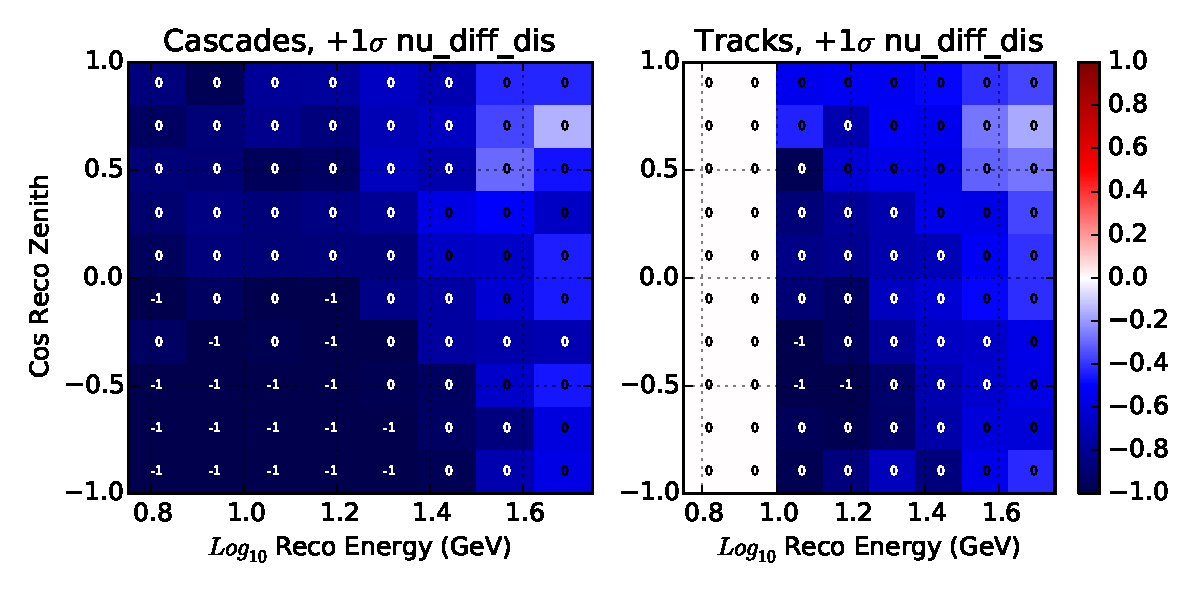
\includegraphics[width=0.9\textwidth]{systematics/nu_diff_dis_variation.pdf} 
\caption[Effect of the neutrino DIS uncertainty in the analysis histogram]{The effect of the DIS uncertainty for neutrinos in the analysis histogram. The colorbar shows the percent change in rate per bin for a shift of 1$\sigma$. The effect is small and largely degenerate with other parameters.}
\label{fig:systematics_nu_dis}
\end{figure}

\begin{figure}
\centering
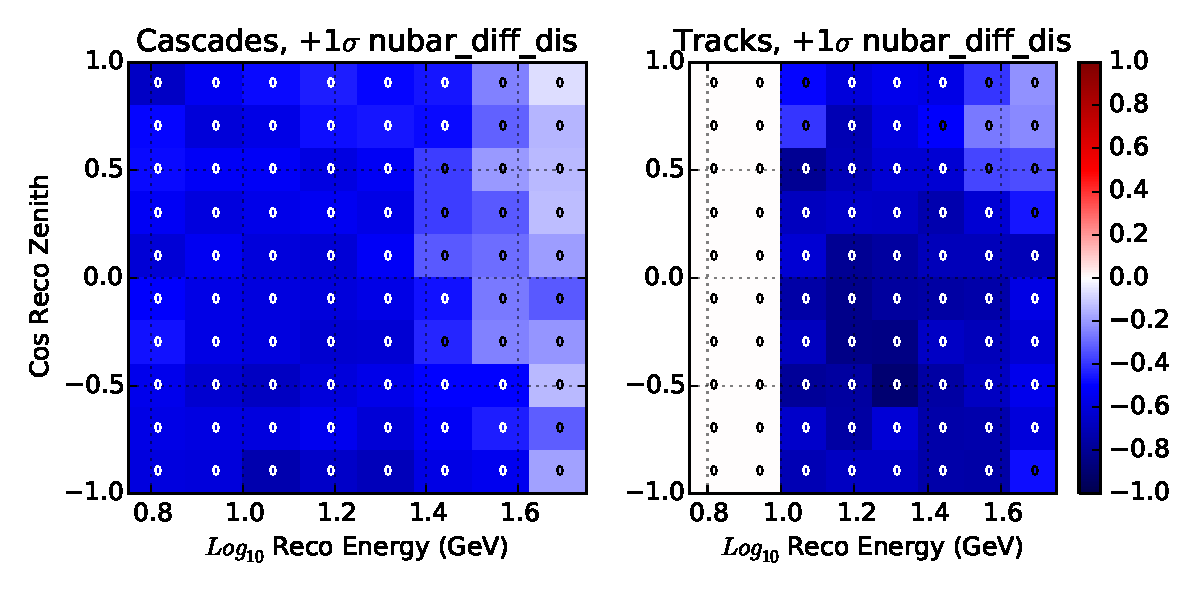
\includegraphics[width=0.9\textwidth]{systematics/nubar_diff_dis_variation.pdf} 
\caption[Effect of the neutrino DIS uncertainty in the analysis histogram]{The effect of the DIS uncertainty for neutrinos in the analysis histogram. The colorbar shows the percent change in rate per bin for a shift of 1$\sigma$. The effect is small and largely degenerate with other parameters.}
\label{fig:systematics_nubar_dis}
\end{figure}

\begin{equation}
x = \frac{Q^2}{2M\nu} , 
\end{equation}

where $Q^2=-q^2$ is the 4-momentum transfer, $M$ is the nucleon mass, and $\nu=E_{had}$ is the energy of the hadronic system \cite{Formaggio-Xsec}.
The GENIE event rate can be corrected to match the NuTeV data using a empirical power law \cite{DIS-Reweighting}:

\begin{equation}
w'_{i} = 
\begin{cases}
(1 - 1.65125 a) x^{-a} w_i & \nu \\
(1 - 1.8073 a) x^{-a} w_i & \bar{\nu}
\end{cases}
\end{equation}

where $a$ is $0 \pm 0.0757$ for neutrinos and $0 \pm 0.1008$ for antineutrinos.
This method has been tested with the GRECO Level 7 dataset.
The resulting uncertainties, shown in Figures~\ref{fig:systematics_nu_dis} and \ref{fig:systematics_nubar_dis}, are small and have large degeneracies with other parameters.
Because of the small size and degeneracy, these systematic uncertainties are not used in the fit.

\label{subsubsec:norm_nc}
\subsubsection{NC/CC Cross Section Ratio}
IceCube is sensitive to both neutral current and charged current interactions.
The uncertainty in the interaction cross section for the charged current is handled with the QE, RES, DIS uncertainties.
To handle the uncertainty in the neutral current cross section, the normalization of neutral current interactions is fit in the tau appearance analysis.
This normalization is measured relative to the charged current rates.

\begin{figure}
\centering
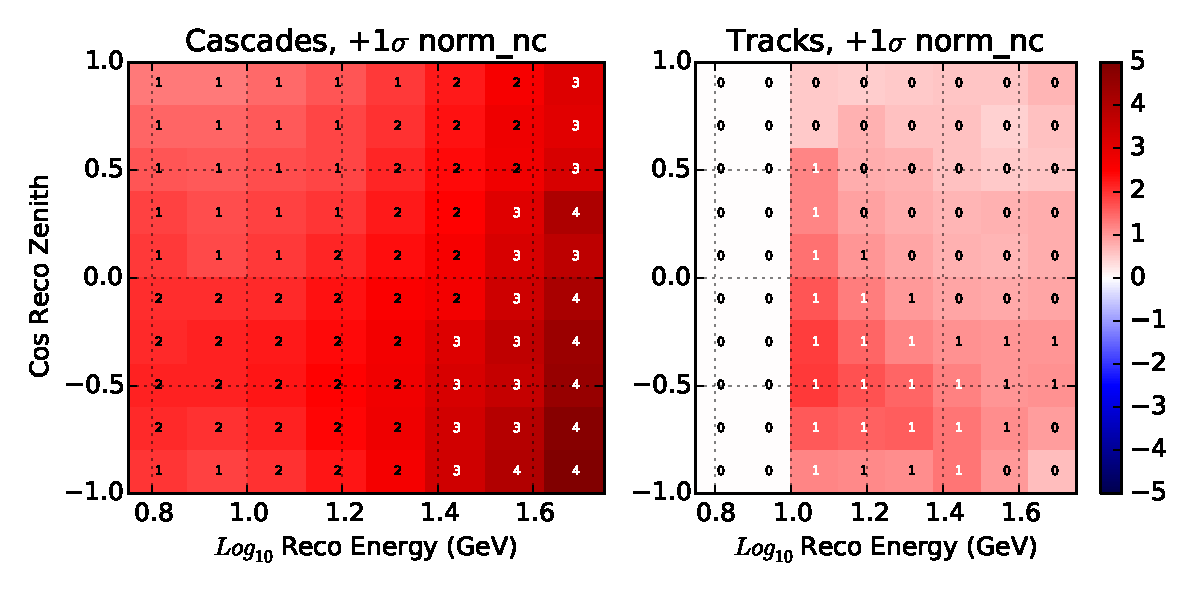
\includegraphics[width=0.9\textwidth]{systematics/norm_nc_variation.pdf} 
\caption[Effect of the neutral current normalization in the analysis histogram]{The effect of the neutral current normalization in the analysis histogram. The colorbar shows the percent change in rate per bin for a shift of 20\%. The effect appears most strongly in the cascade-like sample.}
\label{fig:systematics_norm_nc}
\end{figure}

\begin{equation}
f'_{NC} = N_{NC} \cdot \frac{\sigma_{NC}}{\sigma_{CC}}
\end{equation}

As in previous IceCube analyses, the neutral current normalization is fit with a prior of 1.0~$\pm$~0.2 \cite{IceCube-Oscillation2015,IceCube-Oscillation2018}.
The effects are shown in Figure~\ref{fig:systematics_norm_nc}.


\label{subsec:detector_systematics}
\subsection{Detector Uncertainties}
While the previous systematics uncertainties have been related to global physics parameters, the remainder are dedicated to understanding the uncertainties associated with the IceCube detector itself, such as the properties of the PMTs and the ice.
These parameters, collectively referred to as the \emph{detector uncertainties}, do not have analytic forms, but may affect the rate of events, the reconstruction properties of a given event, or both.
The effect of these uncertainties is evaluated using dedicated Monte Carlo simulations.

The GRECO event selection uses a number of simulation sets, shown in Table~\ref{table:geniesets} for signal and Table~\ref{table:mgsets} for background, to characterize the effects of these Detector Uncertainties.
Each set contains at least one simulation parameter changed from the baseline set and are run through the full GRECO processing.


\subsubsection{Coincident Fraction}
\label{subsubsec:coin_fraction}
The GENIE simulation sets are produced with exactly one neutrino interaction per event. 
In the actual detector, a fraction of triggered events will consist of a temporally coincident muon and neutrino pair which may be from the same air shower or from independent showers.
These events are known as \emph{coincident events}.
In order to account for this possibility, a sample of such events were simulated with independent neutrino and muon generation.
Every produced event contains at least one atmospheric muon in addition to exactly one neutrino interaction.
By interpolating between this "100\% coincident" sample and the standard "0\% coincident" sets, the effect of the coindences is included in the final analysis.

\begin{figure}
\centering
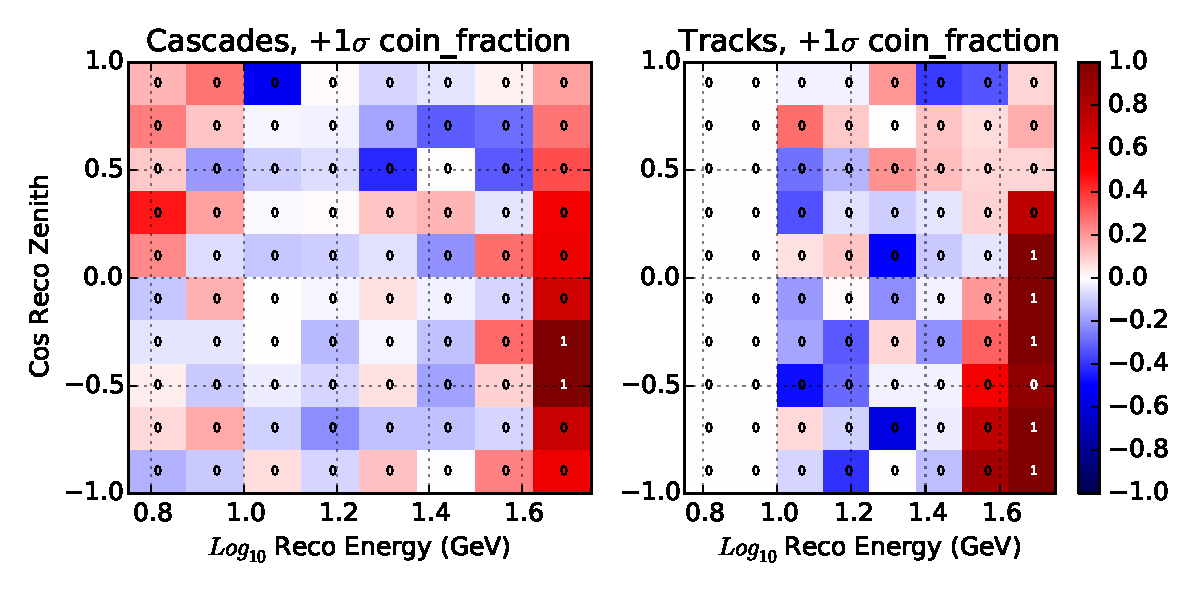
\includegraphics[width=0.9\textwidth]{systematics/coin_fraction_variation.pdf} 
\caption[Effect of the coincident events in the analysis histogram]{The effect of the coincident event rate in the analysis histogram. The colorbar shows the percent change in rate per bin for a shift of 10\%. The parameter is implemented to be independently rate-preserving for each type of neutrino. The coincident event rate induces a small change in the rate of events at high energies.}
\label{fig:systematics_coin_fraction}
\end{figure}

The GRECO event selection is designed to reject atmospheric muon-like events.
Increasing the coincident event fraction leads to a lower total event rate, as events with muons are removed from the selection.
In order to distinguish a change in the analysis histogram due to coincident events from a global normalization factor, the coincident event fraction is implemented to preserve the total number of events of each neutrino type.
The effect of this systematic uncertainty on the binwise event rates in the final analysis is shown in Figure~\ref{fig:systematics_coin_fraction}.

At Final Level, the true fraction of coincident events is unknown, but previous oscillation analyses have found no clear issues using the standard simulation sets assuming no coincident events.
A derivation of the expected coincident event fraction using the atmospheric muon and neutrino rates and assuming the events are produced in independent air showers gives a coincident fraction of 10\%.
A prior is therefore implemented with a one-sided Gaussian distribution centered at 0\% with a 10\% width.

\subsubsection{DOM Efficiency}
\label{subsubsec:domeff}
The \emph{DOM efficiency} is a measure of the total uncertainty in the photon detection probability of IceCube DOMs relative to the expected PMT efficiency.
Prior to deployment, measurements performed with 16 DOMs found an relative uncertainty of 7.7\% on the efficiency of the IceCube DOMs \cite{Description-IceCube}
DOMs measured in-situo using minimum ionizing muons in order to better account for local effects like cable shadowing and the glass-ice interface have found similar uncertainties for the PMT efficiency \cite{Thesis-Feintzeig}.
In this analysis, a conservative estimate of the uncertainty for the DOM efficiency, 99\%$\pm$10\%, is adopted.
The difference between the two uncertainties has been tested and no impact on the tau neutrino appearance measurement was observed.

\begin{figure}
\centering
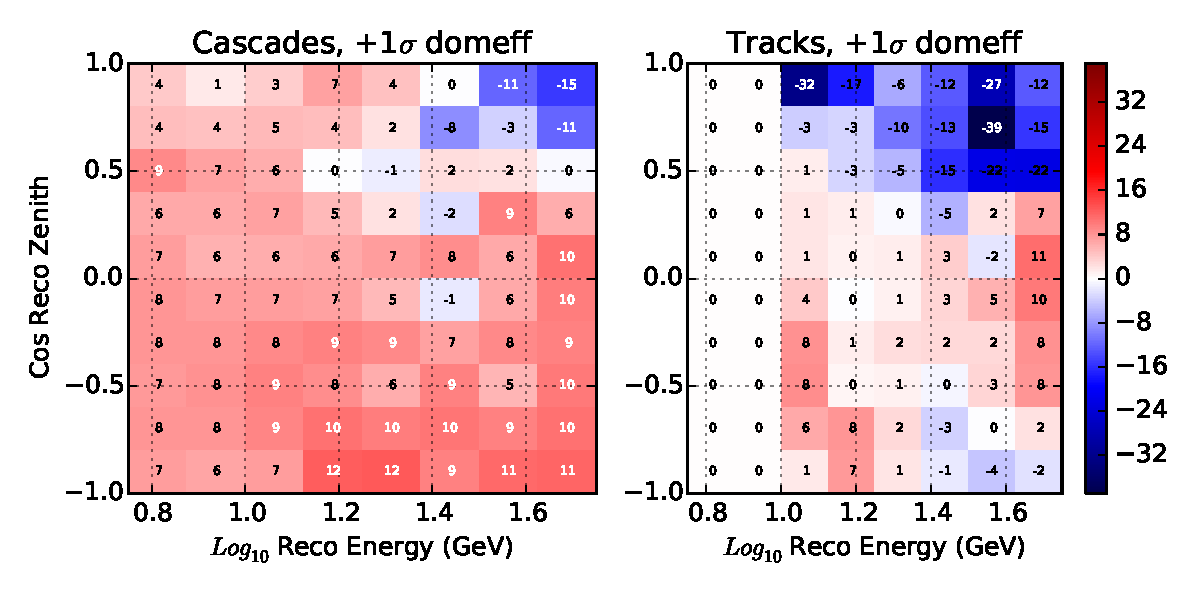
\includegraphics[width=0.9\textwidth]{systematics/domeff_variation.pdf} 
\caption[Effect of the DOM efficiency in the analysis histogram]{The effect of the DOM efficiency in the analysis histogram. The colorbar shows the percent change in rate per bin for a shift of 10\%. The DOM efficiency increases the number of photons observed, improving both the reconstruction resolution and veto efficiency.}
\label{fig:systematics_domeff}
\end{figure}

The DOM efficiency scales the quantum efficiency of observing photons incident at the DOM.
A higher DOM efficiency leads to an increase in the number of observed photons at each DOM, granting more information about particle interactions in the ice.
The improved knowledge of interactions improves the reconstruction of events, increasing neutrino event rates at Final Level and resulting in well-defined oscillation features in the reconstructed energy, zenith, and track length histrograms used for oscillation measurements.
In addition, higher DOM efficiency increases the number of hits observed along atmospheric muon tracks, yielding improved veto efficiency.
The net effect of changing the DOM efficiency by 10\% in the binwise expected event rates is shown in Figure~\ref{fig:systematics_domeff}.

\subsubsection{Bulk Absorption and Scattering}
\label{subsubsec:bulkice}
As described in Section~\ref{sec:bulk_ice}, the bulk ice model used in IceCube is fit in-situo using data from the deployment and detector operation in a process similar to the one described in Section~\ref{sec:vuvuzela_fitting}.
The model consists of scattering and absorption coefficients fit as a function of depth within the detector.
Uncertainties for these scattering and absorption coefficients, shown in Figure~\ref{fig:spicelea}, provide a significant source of uncertainty for physics measurements in IceCube.

To handle these uncertainties at the analysis level, global scale factors are used to modify all scattering or absorption coefficients in the bulk ice model simultaneously.
Using the most recent published uncertainties on our ice model, a total uncertainty of 10\% is assumed for these global scale factors \cite{IceCube-SpiceLea}.
Three systematics sets of scaled scattering and absorption coefficients are used in the GRECO measurement of tau neutrino appearance, corresponding to sets with 10\% larger absorption coefficients, 10\% larger scattering coefficients, and a 7.1\% reduction to both sets of coefficients.

The bulk ice uncertainties have not been tested in previous oscillation analyses \cite{IceCube-Oscillation2013,IceCube-Oscillation2015,IceCube-Oscillation2018}. but both parameters have significant impacts in the appearance analysis.

\begin{figure}
\centering
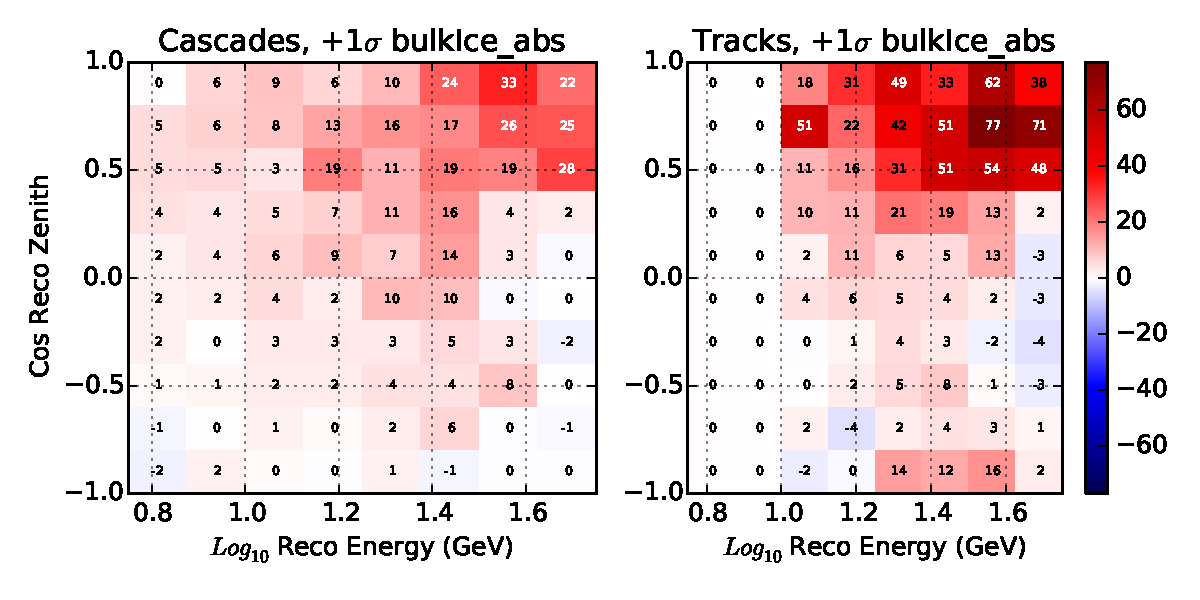
\includegraphics[width=0.9\textwidth]{systematics/bulkIce_abs_variation.pdf} 
\caption[Effect of the absorption in the analysis histogram]{The effect of the absorption in the analysis histogram. The colorbar shows the percent change in rate per bin for a shift of 10\%. The absorption stops photons before they reach DOMs and has similar effects as the DOM efficiency.}
\label{fig:systematics_absorption}
\end{figure}

The absorption, shown in Figure~\ref{fig:systematics_absorption}, is dominated by effects due to atmospheric muons.
This is due to the event selection: with weaker absorption (smaller coefficients), photons travel further in the ice and are more likely to be detected.
The observation of additional photons from the muon track improves the veto efficiency, leading to a significant decrease in the number of muons at Final Level.

\begin{figure}
\centering
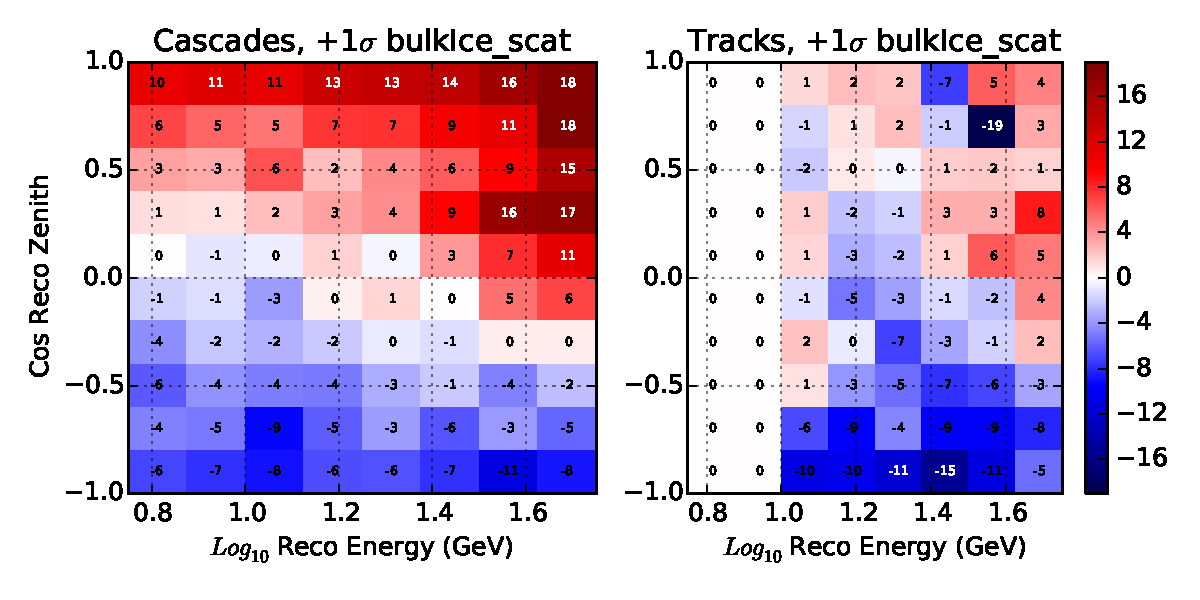
\includegraphics[width=0.9\textwidth]{systematics/bulkIce_scat_variation.pdf} 
\caption[Effect of the scattering in the analysis histogram]{The effect of the scattering in the analysis histogram. The colorbar shows the percent change in rate per bin for a shift of 10\%. The scattering changes the directions of photons as they propagate through the ice. Photons which scatter lose information about the source direction, leading to worse reconstructions. }
\label{fig:systematics_scattering}
\end{figure}

The effect of the scattering is shown in Figure~\ref{fig:systematics_scattering}.
A few bins in the downgoing track-like histogram show strong effects inconsistent with nearby bins. 
These bins arise due tostatistical uncertainty in the parametrizations of the low statistics atmospheric muons sets.
Other than these bins, the scattering does not appear to strongly affect the atmospheric muons.

In the neutrinos, the effects of the scattering are more important.
In particular, stronger scattering (larger coefficients) lead to a reconstruction bias, with more events reconstructing as downgoing.
This is a known effect of the reconstruction, where we use a version of the ice model which interprets off-time hits as being due to backscattered photons in a downgoing event.




\subsubsection{Hole Ice and Foward Scattering}
\label{subsubsec:holeice}
While the bulk ice refers to the scattering and absorption properties of the entire interaction volume, additional care must be taken for the hole ice described in Sections~\ref{sec:hole_ice} and \ref{subsec:holeice_sim}.

The uncertainties associated with the hole ice are some of the most important systematic uncertainties in previous IceCube oscillation analyses \cite{IceCube-Oscillation2018}.
The simulation of the hole ice model used here, discussed briefly in \ref{subsec:holeice_sim}, requires two free parameters which will be referred to as the \emph{hole ice} (p1 in Figure~\ref{fig:angular_acceptance}) and \emph{forward scattering} (p2 in Figure~\ref{fig:angular_acceptance}) parameters.

\begin{figure}
\centering
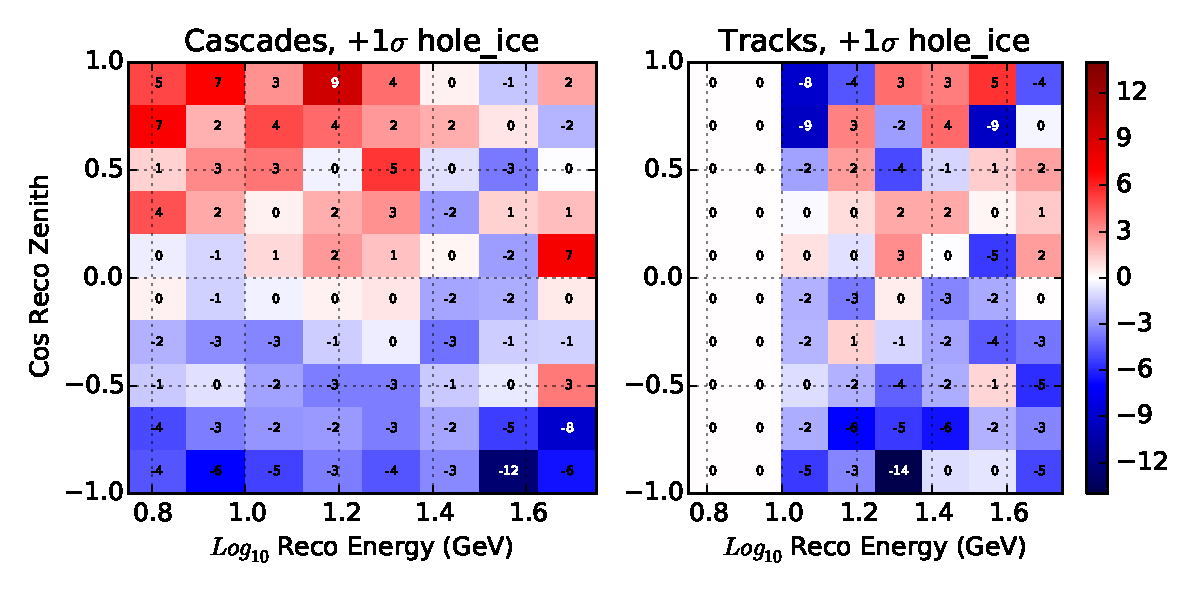
\includegraphics[width=0.9\textwidth]{systematics/hole_ice_variation.pdf} 
\caption[Effect of the hole ice parameter in the analysis histogram]{The effect of the hole ice systematic uncertainty in the analysis histogram. The colorbar shows the percent change in rate per bin for a shift of 1$\sigma$. The hole ice parameter affects the efficiency of detecting photons at the side of the DOM. This parameter changes the angular distribution of photons at the DOM, leading to differences in the resolution of events.}
\label{fig:systematics_holeice}
\end{figure}

\begin{figure}
\centering
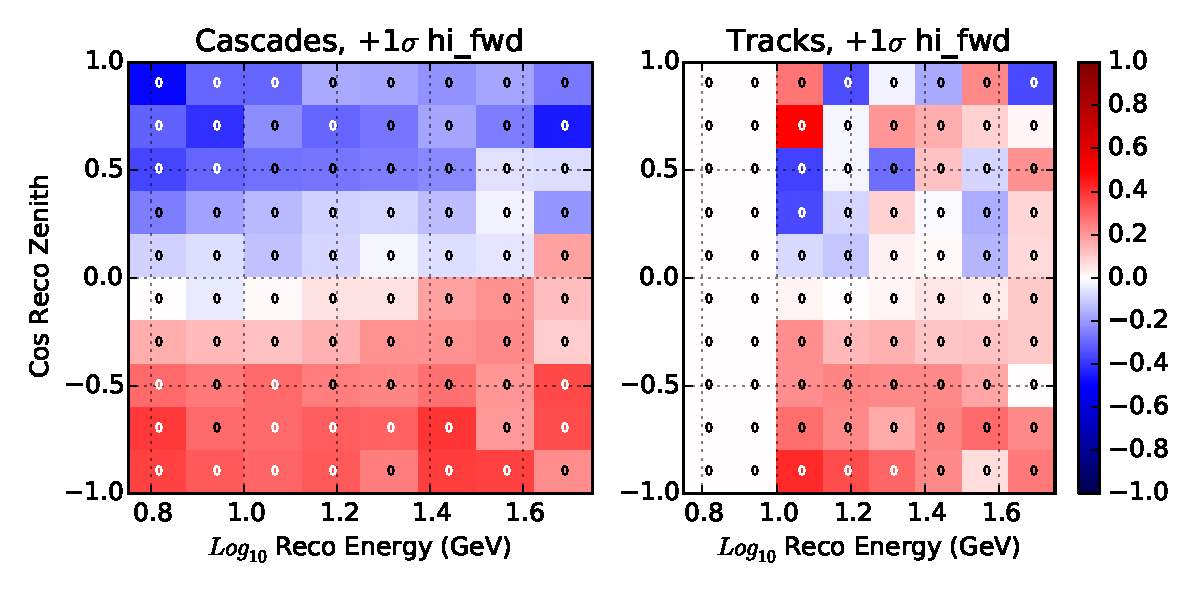
\includegraphics[width=0.9\textwidth]{systematics/hi_fwd_variation.pdf} 
\caption[Effect of the forward scattering parameter in the analysis histogram]{The effect of the forward scattering parameter in the analysis histogram. The colorbar shows the percent change in rate per bin for a shift of 10\%. The forward scattering value affects the efficiency of detecting photons at the front of the DOM. This parameter changes the angular distribution of photons at the DOM, leading to differences in the resolution of events.}
\label{fig:systematics_hi_fwd}
\end{figure}


The models of the angular acceptance were shown previously in Figure~\ref{fig:angular_acceptance}).
The hole ice parameter, shown in Figure~\ref{fig:systematics_holeice}, modifies the efficiency of accepting photons incident from the horizon at each DOM while the forward scattering, shown in Figure~\ref{fig:systematics_hi_fwd}, modifies only the acceptance of the very-forward region.

The effects of the two hole ice parameters show similar behavior to that of the scattering uncertainty in the bulk ice, as all three coefficients are modeling the scattering properties of different locations in the ice.
Tests performed using the GRECO sample have shown that the three parameters are sufficiently distinct to include all three.










\label{sec:likelihood}
\section{The Test Statistic for the Analysis}
The measurement of tau appearance includes many systematics parameters.
To obtain the best fit set of values, a minimization is performed using a $\chi^2$ test statistic.
The form of the $\chi^2$, which includes terms related to the limited simulation statistics available, is described here.

\label{subsec:chi2}
\subsection{The $\chi^2$ Fit}
The $\chi^2$ is a test statistic used to describe the agreement between two binned histograms.
In defining the $\chi^2$, the observed number of events in each bin of the histogram is assumed to be independently gaussian distributed with mean $\mu=\sum_j^{Evts}w_j$ equal to the expected number of events in simulation.

\begin{equation}
	P\left(x|\mu\right) = N e^{\frac{\left(x-\sum_j^{Evts}w_j\right)^2}{\sigma^2}}
\end{equation}

where $N$ is a normalization constant and $x$ is the number of events observed in data.
The variance within the bin is described by the Poisson uncertainty in the bin calculated as the sum of the weights 

\begin{equation}
\label{eqn:sigma_nomc}
	\sigma^2_P = \mu = \sum_j^{Evts}w_j
\end{equation}

The $\chi^2$ may be defined by calculating the log-likelihood of the gaussian distribution.

\begin{equation}
	log\left(L\left(\mu | x\right)\right) = log\left(N\right) + \frac{\left(x-\sum_j^{Evts}w_j\right)^2}{\sigma^2_P}
\end{equation}

The first term is a constant and can be dropped. 
The remainder gives the definition of the standard $\chi^2$ test statistic used for minimization.
This is summed over all bins $i$ to obtain a single value describing the agreement between the data and expectation.
The standard $\chi^2$ calculation is then

\begin{equation}
	\chi^2 = \sum^{bins}_i \frac{\left(x_i-\sum_j^{Evts}w_{ij}\right)^2}{\sum_j^{Evts}w_{ij}} .
\end{equation}

\label{subsec:finite_stats}
\subsection{Finite Statistics}
The $\chi^2$ distribution implicitly assumes that the dominant source of uncertainty at the best-fit point comes from the statistical fluctuations of the data around the true distribution represented by the Monte Carlo simulation.
The statistical properties of the background simulation sets cannot be ignored for the tau neutrino appearance analysis, however.

The statistical fluctuations of the simulation are negligible when the simulated livetime provides at least an order of magnitude larger simulation statistics than expected from the data itself.
Additional simulated statistics may be produced to reduce fluctuations in the Monte Carlo histograms.
In the situation where this is infeasible, modifications to the likelihood space itself can be used to account for the additional uncertainties.
For this analysis, the statistical uncertainty due to finite simulation statistics, $\sigma^2_{FS}~=\sum_j^{Evts} w_j^2$, is added to the weighted uncertainties in quadrature.
This results in a modification of Equation~\ref{eqn:sigma_nomc}.

\begin{equation}
\label{eqn:sigma_mc}
	\sigma^2 = \sigma^2_P + \sigma^2_{FS} =  \sum_j^{Evts} w_j + w_j^2
\end{equation}

This changes the definition of the $\chi^2$ to

\begin{equation}
\label{eqn:mchi2}
	\chi_{FS}^2 = \sum_i^{bins} \frac{\left(x_i-\sum_j^{Evts} w_{ij}\right)^2}{\sum_j^{Evts}w_{ij} + \sum_j^{Evts}{w_{ij}^2}}
\end{equation}		
%
were "finite statistics" subscript $FS$ has been introduced to distinguish this value from the standard $\chi^2$.
This can be rewritten explicitly in terms of the atmospheric muon and neutrino samples

\begin{equation}
	\chi_{FS}^2 = \sum_i^{bins} \frac{\left(x_i- \sum_j^{Evts} \left( \left(w_{ij}\right)_\nu - \left(w_{ij}\right)_\mu\right) \right)^2}
		{\sum_j^{Evts}\left(w_{ij}\right)_\nu + \left(w_{ij}\right)_\mu + \left(w^2_{ij}\right)_\nu +\left(w^2_{ij}\right)_\mu}
\end{equation}	

Test minimizations performed with the $\chi^2$ form of Equation~\ref{eqn:mchi2} presented a unique problem.
Because the muon statistical uncertainty is large, fit parameters which increase the weight of muon events increase the denominator of the $\chi^2$.
This was found to occur with the DOM efficiency and absorption systematic parameters, leading to a runaway minimization in Monte Carlo trials where the DOM efficiency was shifted by more than 5$\sigma$ and the $N_{\nu_\tau}$ was biased by more than 40\%.

In order to prevent this runaway effect, a further modification of the $\chi^2$ is required.
For this analysis, the total scale of the statistical uncertainty due to atmospheric muons, $\sigma^2_{FS, \mu}$, is fixed the seed values of the fit.

\begin{equation}
\label{eqn:w2_constant}
	N^\mu_i = \frac{\left(\sum_j^{Evts} w_{ij}^2\right)_{Seed}}{\sum_j^{Evts} w_{ij}^2}
\end{equation}

Inserting this term into the denominator, one obtains the form of the $\chi^2_{FS}$ 

\begin{equation}
\label{eqn:chi2_final}
	\chi^2_{FS} = \sum_i^{bins} \frac{\left(x_i-\sum_j^{Evts} w_{ij}\right)^2}{\sum_j^{Evts}w_j + \left(\sum_j^{Evts}{w_{ij}^2}\right)_\nu + N^\mu_i\left(\sum_j^{Evts}{w_{ij}^2\right)_\mu}} 
\end{equation}


With this modification, the $\chi^2$ minimization is well-behaved.



\subsection{Fit Priors}
Prior knowledge of some systematics parameters can be included in the fit using a \emph{prior}.
Priors are additional terms included multiplicatively (additively) in the likelihood (log-likelihood) calculation that represent one's belief about the likely value of the systematics.
These often take the form of a gaussian distribution with mean $\mu$ and variance $\sigma^2$ given by external measurements.
In the search for appearance, most priors are handled assuming a standard gaussian form.
For a systematic $m$ with value $x_m$, these additional terms take the form

\begin{equation}
	\chi^2_{m} =  \frac{\left(x_m-\mu\right)^2}{\sigma_m^2}
\end{equation}

These additional terms are added to Equation~\ref{eqn:chi2_final} in order to calculate the final $\chi^2_{FS}$ used in the minimization for this analysis.

\begin{equation}
	\chi^2_{Total} = \sum_i^{bins} \left(\chi^2_{FS}\right)_i + \sum_m^{syst} \chi^2_{m}
\end{equation}

A list of priors is shown in Table~\ref{tab:priors}.
Note that the coincident event fraction is effectively a one-sided Gaussian due to physical constraints on the value.


\begin{landscape}
\begin{table}[]
\centering
\begin{tabular}{@{}llllllll@{}}
\toprule
                               & Systematic                            & Unit                        & Type       & Baseline/Seed Value     & Prior           & Allowed Range & Reference                     \\ \midrule
Physics Parameter    & $N_{\nu_\tau}$                    & -                             & Analytic   & 1.0                     & -                       & 0.0 - 2.0     & -                             \\ \midrule
\multirow{2}{*}{Oscillations}  & $\Delta m^2_{3j}$  & $10^{-3}$ $eV^2$ & Analytic   & 2.526                  & -                      & 2.0 - 3.0     & \cite{NuFit.org}            \\
                               & Sin$^2 \theta_{23}$            & -                             & Analytic   & 0.440 (NO), 0.66 (IO)   & -              & 0.0 - 1.0     & \cite{NuFit.org}             \\ \midrule
Total Rates              & $N_\nu$, $N_\mu$              & Years                      & Analytic   & 2.25                    & -                      & 0.0 - 10.0    & -                             \\ \midrule
\multirow{3}{*}{Cross-section} & Axial Mass (QE)     & $\sigma$                & Analytic   & 0.0                     & 0.0 $\pm$ 1.0   & -5.0 - 5.0    & \cite{GENIE}             \\
                               & Axial Mass (RES)                    & $\sigma$               & Analytic   & 0.0                     & 0.0 $\pm$ 1.0   & -5.0 - 5.0    & \cite{GENIE}             \\
                               & $N_{\nu^{NC}}$                   & -                            & Analytic   & 1.0                     & 1.0 $\pm$ 0.2   & 0.0 - 2.0     & \cite{IceCube-Oscillation2018}          \\ \midrule
\multirow{6}{*}{Flux}& $\gamma_\nu$                    & -                            & Analytic   & 0.0                     & 0.0 $\pm$ 0.10  & -0.50 - 0.50  & \cite{Honda-2015}         \\
                               & $\gamma_\mu$                   & $\sigma$                & Analytic   & 0.0                     & 0.0 $\pm$ 1.0   & -5.0 - 5.0    & \cite{NuFlux-Manchester}                \\
                               & Up/Horizontal Ratio               & $\sigma$                & Analytic   & 0.0                     & 0.0 $\pm$ 1.0   & -5.0 - 5.0    & \cite{NuFlux-Barr}              \\
                               & $\nu$/$\bar{\nu}$ Ratio       & $\sigma$               & Analytic   & 0.0                     & 0.0 $\pm$ 1.0   & -5.0 - 5.0    & \cite{NuFlux-Barr}             \\
                               & $\Phi_{\nu_e}$                    & -                             & Analytic   & 1.0                     & 1.0 $\pm$ 0.05 & 0.8 - 1.2     & \cite{NuFlux-Barr}              \\
                               & Coincident Fraction                & -                            & Non-analytic & 0.0                     & 0.0 + 0.10        & 0.0 - 1.0     & -                                       \\ \midrule
\multirow{5}{*}{Detector}      & DOM Efficiency        & -                             & Non-analytic & 1.0                     & 1.0 $\pm$ 0.1  & 0.7 - 1.3     & \cite{IceCube-SpiceMie,Thesis-Feintzeig}           \\
                               & Hole Ice                                & -                            & Non-analytic & 0.25                    & 0.25 $\pm$ 0.10 & 0.0 - 0.5  & \cite{IceCube-Oscillation2018}                 \\
                               & Forward Scattering                 & -                            & Non-analytic & 0.0                     & -                        & -5.0 - 5.0    & \cite{IceCube-Oscillation2018}                 \\
                               & Absorption                            & -                            & Non-analytic & 1.0                     & 1.0 $\pm$ 0.1   & 0.5 - 1.5     & \cite{IceCube-SpiceMie}          \\
                               & Scattering                             & -                            & Non-analytic & 1.0                     & 1.0 $\pm$ 0.1   & 0.5 - 1.5     & \cite{IceCube-SpiceMie}         \\ \bottomrule
\end{tabular}
\caption{Priors and allowed ranges for each systematic included in this analysis.}
\label{tab:priors}
\end{table}
\end{landscape}






\label{subsec:fitter}
\subsection{Fitting Code}
In order to understand the expected sensitivity of this analysis, a software fitting package previously used to fit the $\nu_\mu$ disappearance is used \cite{IceCube-Oscillation2013,IceCube-Oscillation2015,IceCube-Oscillation2018,}.

The code, known as \emph{OscFit}, works in multiple stages.
After separating the simulation into separate channels consisting of $\nu_e^{CC}$, $\nu_\mu^{CC}$, $\nu_\tau^{CC}$, $\nu^{NC}$, $\mu_{atm}$, and accidental triggers, the analytic systematics are applied.
These systematics solely rely on information about the particle interaction in order to calculate correction factors to the event weights and are not sensitive to the order of application.
The oscillation calculations are performed as analytic systematics based on the Prob3++ code \cite{prob3} to calclulate the full three-flavor unitary oscillations including matter effects within the Earth using a reference model of the Earth \cite{PREM}.

When including the neutral current interactions from tau neutrino events in the signal definition and fitting $N_\tau^{NC+CC}$, the neutral current events are reweighted for oscillations at this stage.
The OscFit code assumes the neutral current interaction rate is unaffected by oscillations and instead models neutral current interactions using only muon neutrino and electron neutrino simulated neutral current events.
Because no charged leptons are produced in the neutral current interactions, no differences in event topology are expected based on flavor of neutrino interaction.

For the purposes of this analysis, the neutral current interactions from electron neutrino and muon neutrino events are used to model the effect of the tau neutrino neutral current events.
The Prob3++ code calculates oscillation probabilities for the muon and electron neutrino events to oscillate to tau neutrinos.
These probabilities are used to identify a sample of neutral current events used to model the tau neutrino neutral current interactions.

The modification to the muon neutrino neutral current event weight given the tau neutrino normalization, $N_{\nu_\tau}$, is then given by

\begin{equation}
\begin{aligned}
	w_{i, \nu_\mu^{NC}}^\prime ={}& w_{i, \nu_\mu^{NC}}  \\ 
													{}&- w_{i, \nu_\mu^{NC}}\ P_{\nu_\mu\rightarrow\nu_\tau}\left(E_i, \cos(\theta_i) \vert \Delta m^2_{3j}, \theta_{23} \right) \\ 
													{}&+ N^{NC+CC}_{\nu_\tau}\ w_{i, \nu_\mu^{NC}}\ P_{\nu_\mu\rightarrow\nu_\tau}\left(E_i, \cos(\theta_i) \vert \Delta m^2_{3j}, \theta_{23} \right) 
\end{aligned}
\end{equation}
%
where $w_{i, \nu_\mu^{NC}}$ and $w_{i, \nu_\mu^{NC}}^\prime$ are event weights before and after application of the neutral current oscillations, $E_i$ and $\cos(\theta_i)$ are the energy and zenith angle of the event, and $\Delta m^2_{3j}$ and $\theta_{23}$ are the atmospheric mass splitting and mixing angle respectively.
The first term corresponds to the unoscillated muon neutrino neutral current weight.
The second and third terms correspond to the muon neutrino disappearance and tau neutrino appearance in the neutral current channel respectively.
The oscillation weighting of the neutral current electron neutrinos events follows the same form.

After oscillations and other analytic systematic uncertainties are applied, the events are binned in energy, zenith, and track length with one histogram per simulated channel type.
The non-analytic systematic uncertainties are applied to the each of the binned templates bin-by-bin using hyperplanes calculated as described in Section~\ref{subsec:hyperplanes}.

Once all systematic uncertainties have been applied, the normalization terms representing the overall scale factors for the neutrino rate, $N_\nu$, the muon rate, $N_\mu$, and the accidental rate, $N_{noise}$, are multiplied to the respective histograms.
The final histograms are summed together to form the final simulation expectation to be compared to the data using the $\chi^2_{FS}$ described in Equation~\ref{eqn:chi2_final}.

The value of the $\chi^2_{FS}$ is minimized as a function of the various systematics using the iMinuit2 package \cite{iminuit-paper,iminuit-code}.
The minimization continues until the requested tolerance, $10^{-16}$, is reached by the minimizer, after which the best fit histogram and systematics values are returned to the user.








\label{sec:sensitivity}
\section{Expected Sensitivity to Appearance}
With the full set of systematics included, the \emph{sensitivity} of the analysis is calculated.
The sensitivity is a measure of the expected result and can be performed with simulated events prior to the final fit to data.

To evaluate the expected sensitivity of this analysis, the OscFit code is used to find the best-fit value of the $\chi^2_{FS}$.
Multiple methods are used to evaluate both the average expected sensitivity and range of variation of the sensitivity due to both the data and simulation statistics.
A summary of the results using all methods is shown in Figure~\ref{fig:mc_sensitivity}
Each component will be described in turn.

\begin{figure}[h]
\centering
\begin{tabular}[b]{c}
  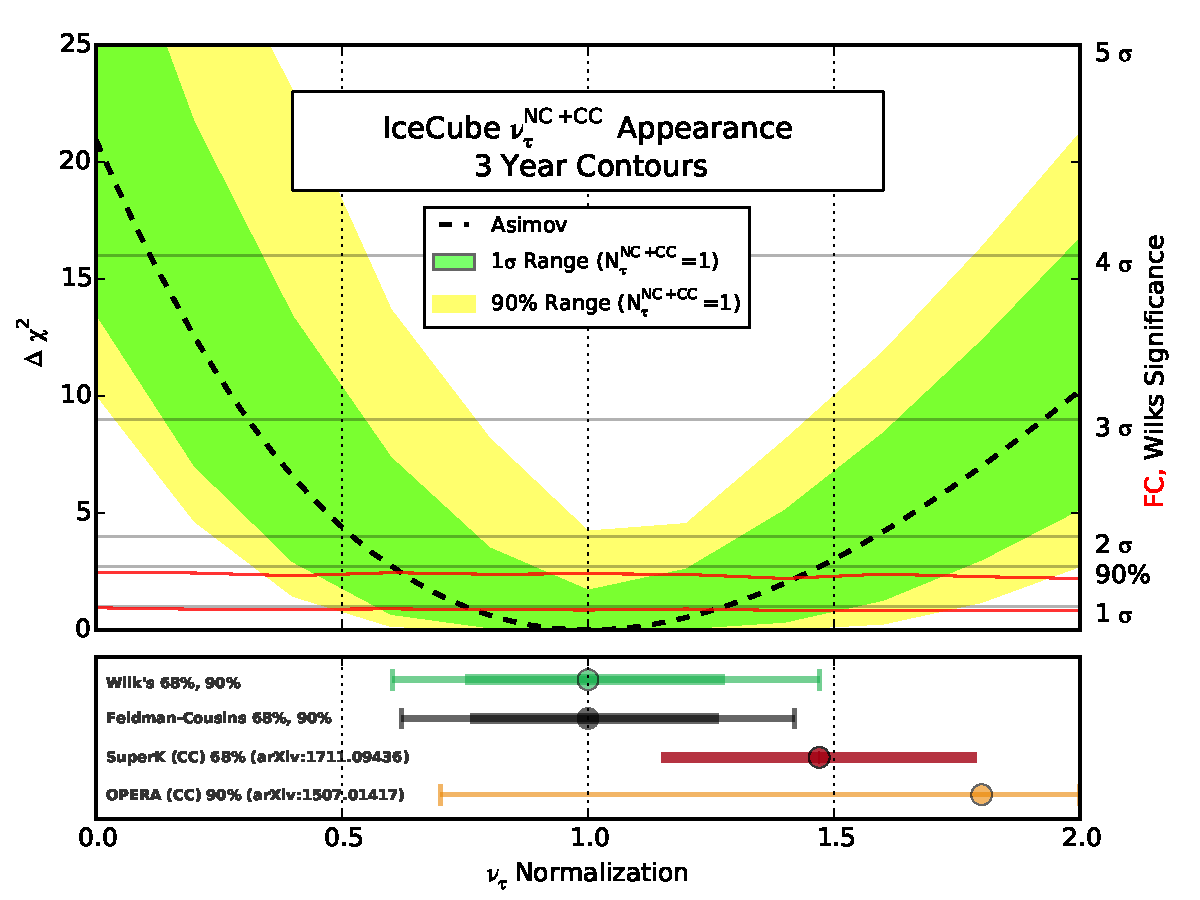
\includegraphics[width=0.45\linewidth]{nc_cc_feldman_cousins.pdf} \\
  \small (\textbf{\color{ctcolormain}a}) NC+CC 
\end{tabular} \hspace{2pt}
\begin{tabular}[b]{c}
  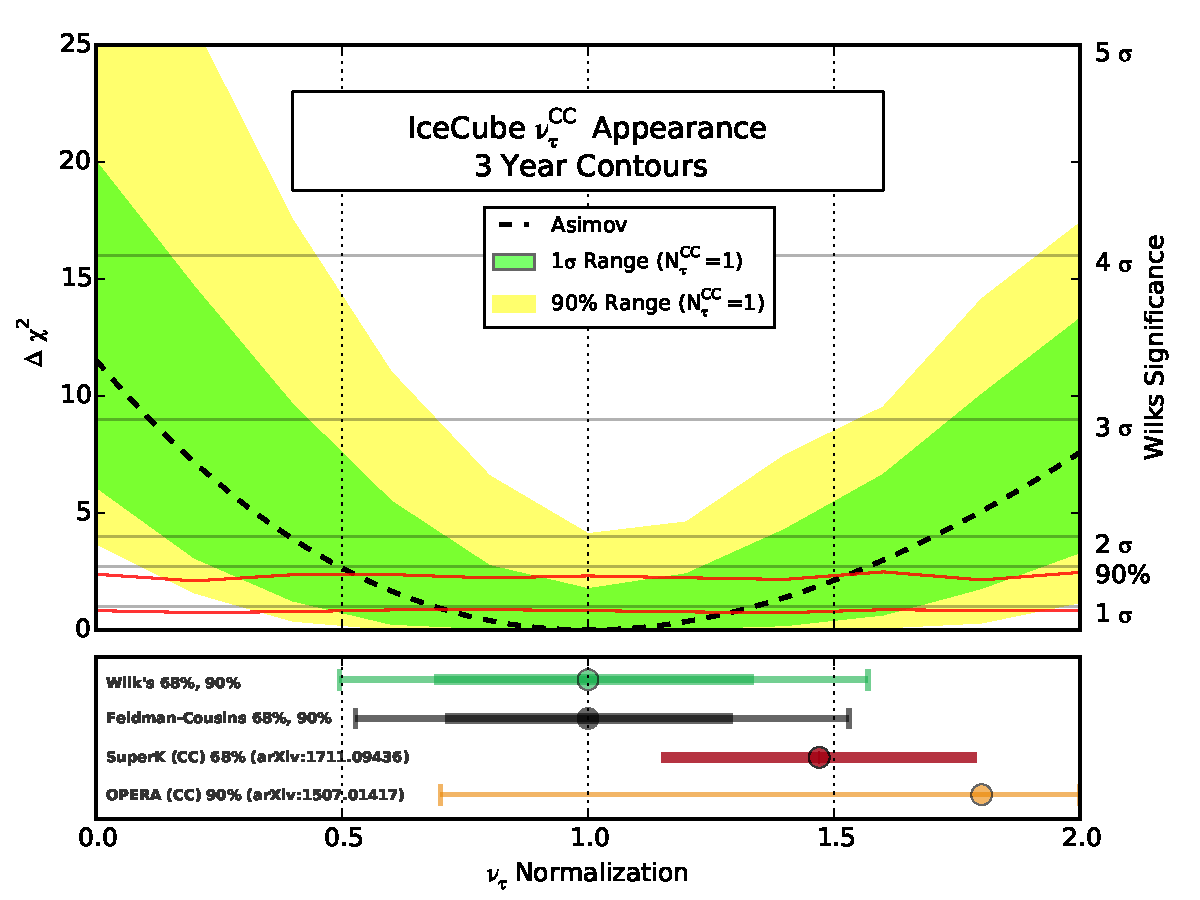
\includegraphics[width=0.45\linewidth]{cc_feldman_cousins.pdf} \\
  \small (\textbf{\color{ctcolormain}b}) CC Only
\end{tabular}
	\caption{The sensitivity of this analysis in the (a) NC+CC and (b) CC-only channel. The top plot shows the Asimov expectation (black dotted line) and the Brazilian flag (green, yellow bands). The significances assuming Wilk's theorem (gray horizontal lines) and Feldman-Cousins (red horizontal lines) are also shown. The bottom plot shows the expected 1$\sigma$ and 90\% ranges for Wilks theorem and Feldman-Cousins compared to the most recent results from the OPERA and Super-Kamiokande analyses.}
	\label{fig:mc_sensitivity}
\end{figure}

\label{subsec:asimov}
\subsection{The Asimov Dataset}
The first method, known as the \emph{Asimov} expectation \cite{Asimov}, begins by creating the expected histogram using baseline values of the systematics and oscillations.
The produced histogram, representing an exact PDF of the expected events, is then used as an estimate of the data.
A scan is performed over values of  $N_{\nu_{\tau}}$, minimizing the $\chi^2_{FS}$ at each point to produce a contour.
A final minimization is performed allowing the minimizer to identify the global best-fit value of $N_{\nu_{\tau}}$.

The final expected sensitivity in the Asimov approach is given by calculating the $\Delta \chi^2$ between the values of the $\chi^2_{FS}$ at each point and the global best fit.

\begin{equation}
\label{eqn:delta_chi2}
	\Delta \chi^2 \left(N_{\nu_{\tau}}\right) = \chi^2_{FS}\left(N_{\nu_{\tau}}\right)  - \chi^2_{FS}\left(N^{Global}_{\nu_{\tau}}\right)
\end{equation}

The value of $\Delta \chi^2_{FS}$ as a function of $N_{\nu_{\tau}}$ is shown by the dotted black line in Figure~\ref{fig:mc_sensitivity}.
These values may be converted into expected significance levels using the procedure described in Section~\ref{subsec:wilks}.




\label{subsec:flag}
\subsection{The Brazilian Flag}
The second method, producing what is known as a \emph{Brazilian flag} plot due to the color scheme, provides an estimate of the statistical uncertainty on the Asimov sensitivity.
The production of a Brazilian flag begins with the production of a pseudo-data histogram from the Asimov histogram.

Because the simulation sets used here have significant uncertainties due to limited simulation statistics in the background samples, the first step is to vary the event rate in each bin within the statistical uncertainties of the Monte Carlo.

A new realization of the simulation histogram is produced by sampling new rates in each bin using a gaussian distribution with mean $\mu_i=\sum_j^{Evts}w_{ij}$ and variance $\sigma^{MC}_{i}$ given by 

\begin{equation}
	\sigma^{2}_{i} = \sqrt{\sum_j^{Evts} w^2_{ij}} .
\end{equation}

The new histograms are them summed together and a final rate in each bin is sampled from a Poisson distribution with mean equal to the new expectation, creating a representation of one possible realization of the data in the analysis.
The OscFit minimization then proceeds as described in the Asimov case for each of 500 realizations of pseudo-data, with the calculation of the $\Delta \chi^2$ as described in Equation~\ref{eqn:delta_chi2}.
The Brazilian flag shows the 1$\sigma$ and 90\% range of $\Delta \chi^2$ values at each value of $N_{\nu_{\tau}}$.
This provides a graphical representation, shown in the colored bands of Figure~\ref{fig:mc_sensitivity}, of the expected range of variation of the sensitivity given solely statistical uncertainties.


\label{subsec:wilks}
\section{Feldman-Cousins vs Wilk's Theorem}
Estimates of the sensitivity of the analysis were performed using a theorem by Samuel S. Wilks \cite{wilks}.
The theorem describes the distribution of the log-likelihood ratio when fits form a "nested model" where fit parameters used in one fit hypothesis, ${H_0}$, form a complete subset of those used in another fit hypothesis, H.
If the two likelihoods used in the log-likelihood ratio differ by N parameters, Wilk's theorem states that the distribution of the test statistic $\Delta \chi^2$ will asymptotically approach a chi-squared distribution with N degrees of freedom.

In the case of the measurement of tau neutrino appearance, fits are performed twice in order to obtain the log-likelihood ratio: once with the value of ${N_{\nu_\tau}}$ fixed to various points and once with ${N_{\nu_\tau}}$ freely floating.
The $\Delta chi^2$ is calculated at each fit point relative to the overall best-fit likelihood using Equation~\ref{eqn:delta_chi2}.
These two fits form a nested model with N=1, allowing the application of Wilk's theorem to estimate significances.

Wilk's theorem gives a useful estimate of the significance and requires negligible additional computational power.
However, the theorem states only an asymptotic limit and assumes that the nested hypotheses are from boundaries and have no discrete steps.
Evaluation of the applicability of Wilk's theorem requires a more robust analysis using Monte Carlo trials.

A procedure, introduced by Gary Feldman and Robert Cousins \cite{feldman_cousins}, can be applied instead.
Instead of assuming a number of degrees of freedom, the Feldman-Cousins procedure requires directly using the distribution of the $\Delta \chi^2_{FS}$ test statistic in order to evaluate the significance.
For IceCube oscillation results, a method similar to the procedure by Feldman and Cousins is used \cite{IceCube-Oscillation2018}.

To begin, a value of ${N_{\nu_\tau}^{True}}$ is selected.
Monte Carlo trials are produced with this true value and the $\Delta \chi^2$ between the best-fit value of ${N_{\nu_\tau}}$ and ${N_{\nu_\tau}^{True}}$ for each trial is calculated.
The distribution of the $\Delta \chi^2_{FS}$ values is used to identify the value of $\Delta \chi^2_{FS}$ below which ${P_{i=1\sigma}\left(\Delta \chi^2_{FS}\right) \approx 68.27\%}$ of trials lie.
This value is the 1${\sigma}$ level for the chosen value of ${N_{\nu_\tau}^{True}}$.
The procedure is repeated for each required value of ${N_{\nu_\tau}^{True}}$ and different significance levels ${i}$.

Examples of the likelihood ratio distribution for various values of ${N_{\nu_\tau}^{True}}$ are shown in Figure~\ref{fig:llh_ratio_dist}.
A ${\chi^2}$ distribution with 1 degree of freedom is overlaid, showing the expected distribution assuming Wilk's theorem. 
The difference in location of the 90\% level from Wilks (green) and Feldman-Cousins (red) is also shown.
The distributions show a preference for a slightly narrower distribution than expected from Wilk's theorem.
The difference indicates that the Feldman-Cousins procedure is necessary to correctly characterize the final result.

\begin{landscape}
\begin{figure}
\centering 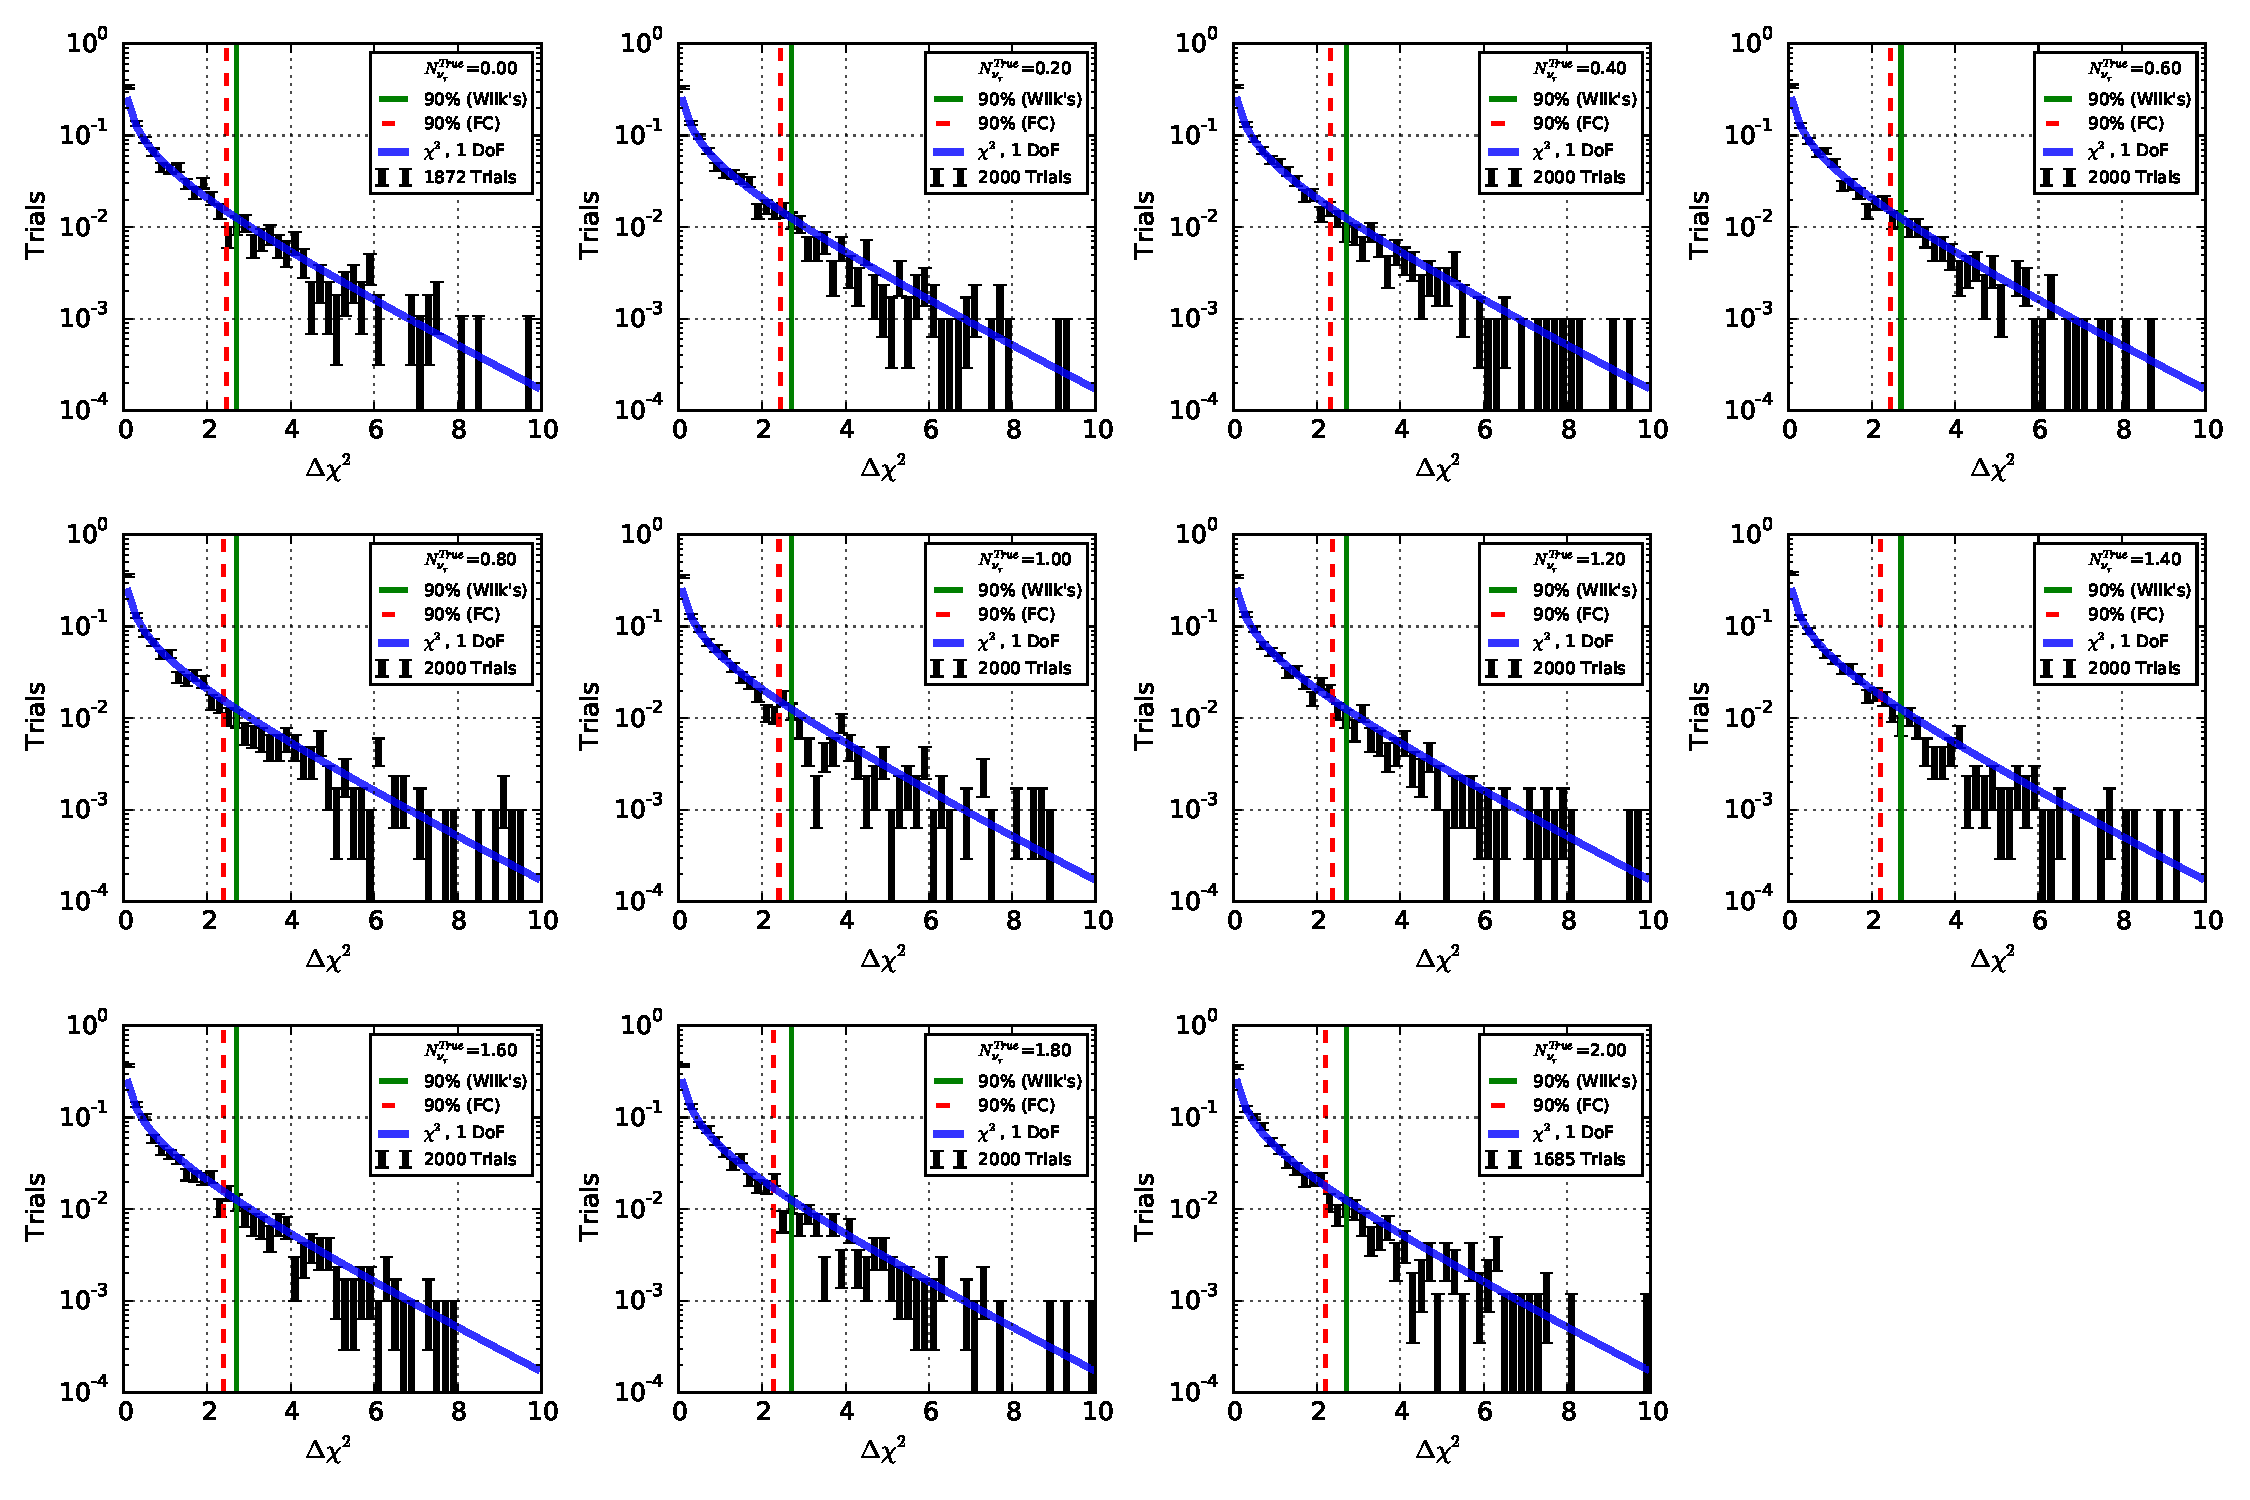
\includegraphics[width=1.2\textwidth]{fc_nc.pdf}
\caption[$\Delta \chi^2_{FS}$ distributions for 11 points in ${N_{\nu_\tau}^{True}}$]{The distributions the $\Delta \chi^2_{FS}$ for 11 points in ${N_{\nu_\tau}^{True}}$ in the NC+CC fit. The assumption of 1 degree of freedom from Wilk's theorem is tested at the location of ${\left(\Delta \chi^2_{FS}\right)_{90\%}}$ for each point. The distribution calculated from Monte Carlo trials is narrower than that predicted by Wilk's theorem, indicating that a more complete treatment with the Feldman-Cousins procedure is necessary.}
\label{fig:llh_ratio_dist}
\end{figure}
\end{landscape}

The evaluated ${\left(\Delta \chi^2_{FS}\right)_i}$ are limited to the discrete values chosen in ${N_{\nu_\tau}^{True}}$.
In order to obtain a continuous model, a cubic spline is used to interpolate the values of ${\left(\Delta \chi^2_{FS}\right)_i}$ as a function of $N_{\nu_\tau}^{True}$.
Similarly, the contour from data fit to a cubic spline for interpolation. 
The crossing points of the two splines is the best estimate for the uncertainty of the final result.

The procedure does not rely on assumptions about the distribution of the $\Delta \chi^2_{FS}$ values and works in cases where the likelihood ratio distribution is not chi-squared distributed.
The number of trials required to reduce the effect of statistical fluctuations in the evaluation, however, can make such evaluations prohibitively expensive.

A total of 1000 trials at each point are evaluated for the fits to both $N_{\nu_\tau}^{CC}$ and $N_{\nu_\tau}^{NC+CC}$.
All trials were produced assuming the baseline values of each systematic and with $N_{\nu_\tau}=1$.
The resulting values of $\left(\Delta \chi^2_{FS}\right)^i_{FC}$ are shown in the red lines in Figure~\ref{fig:mc_sensitivity}.





\label{sec:systematics_impact}
\section{Impact of Systematic Uncertainties}
There are various ways to measure the impact of the included systematics in this analysis.
Described here are methods to evaluate, in order of increasing importance, the total systematics impact, the impact of each systematic individually, the correlation between systematics, and the effect of non-baseline values.
Each of these test different aspects of the sensitivity and all are included for completeness.

\subsubsection{Total Impact of Systematic Uncertainties}
The total impact of the systematics on the sensitivity is measured by comparing the total Asimov sensitivity to an Asimov sensitivity calculated using no systematic uncertainties.
This is shown at the bottom of Figure~\ref{fig:n+1_tests}.
It is clear from the comparison that the analysis is very sensitive to the included systematics set.

\subsubsection{N+1 Tests: Sensitivity of Analysis to Systematic}
\begin{figure}[h]
\centering
\begin{tabular}[b]{c}
  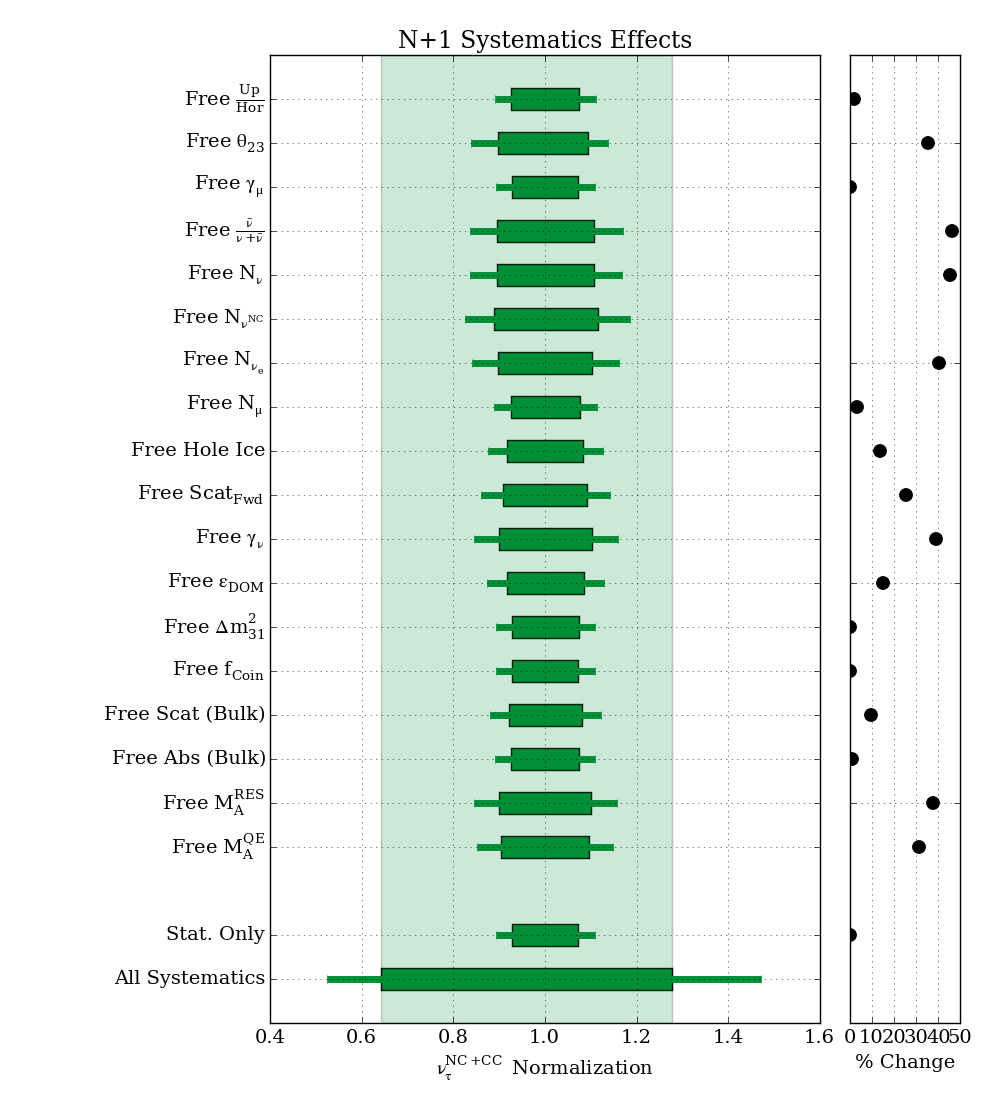
\includegraphics[width=0.45\linewidth]{n+1_widths_nc_cc.png} \\
  \small (\textbf{\color{ctcolormain}a}) NC+CC
\end{tabular} \hspace{2pt}
\begin{tabular}[b]{c}
  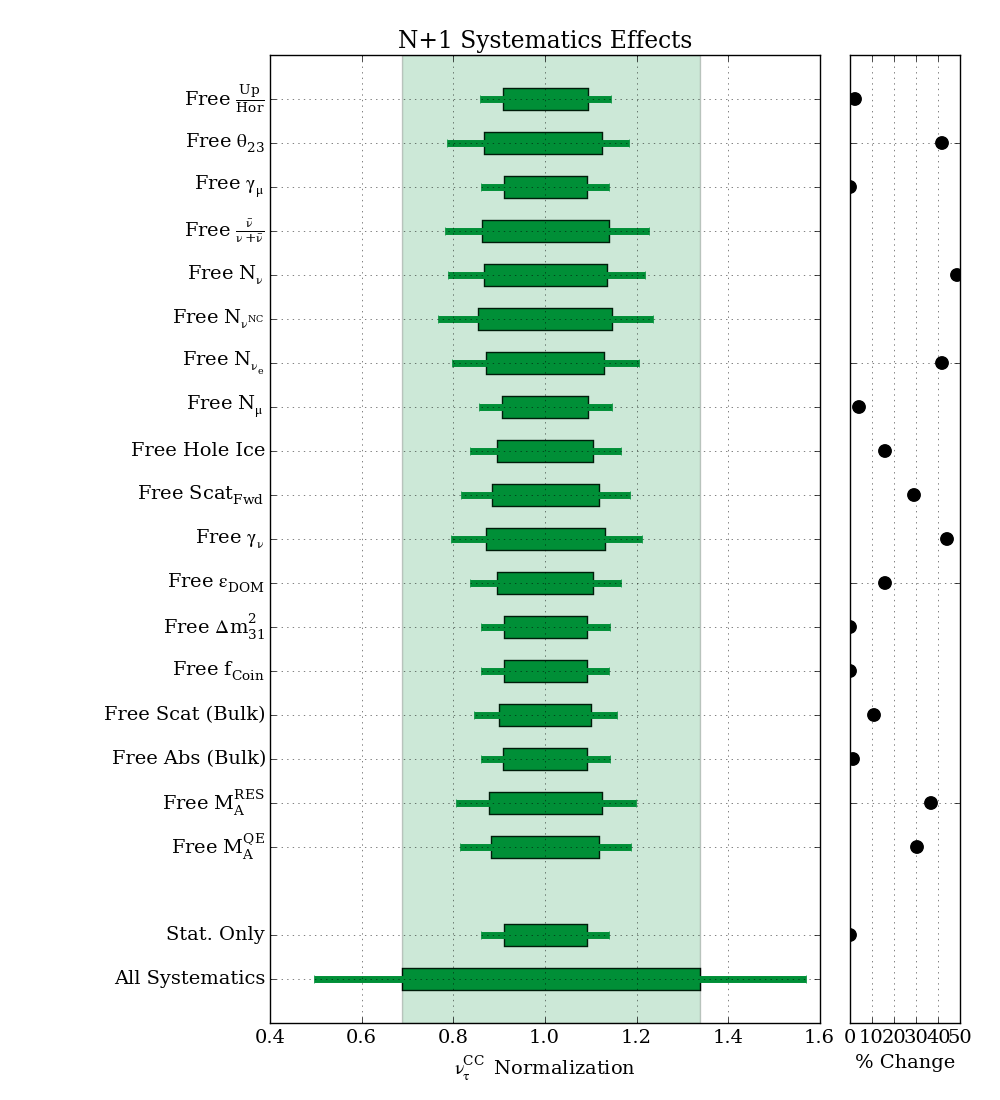
\includegraphics[width=0.45\linewidth]{n+1_widths_cc.png} \\
  \small (\textbf{\color{ctcolormain}b}) CC Only
\end{tabular}
\caption[The N+1 parameter tests]{The N+1 parameter tests for (a) the NC+CC fit and (b) the CC-only fit. Only one parameter is allowed to move at a time. The change in the 1$\sigma$ and 90\% expected confidence intervals give an indication of the strength of each systematic parameter in isolation.}
\label{fig:n+1_tests}
\end{figure}

A different test is also possible: Instead of calculating likelihoods with no systematic uncertainties included, a single systematic uncertainty is used at a time.
This test, called an N+1 test for the addition of one uncertainty at a time, yields useful information on a sample's sensitivity to single systematic parameters.
The results of the N+1 tests are shown in Figure~\ref{fig:n+1_tests}.

A small change in sensitivity between the "no systematic uncertainties" case above and an N+1 Asimov sensitivity may have two possible explanations.
The first that the current analysis is unaffected by changes in the systematic parameter, implying that the systematic uncertainty should be investigated for removal in the analysis.
The second possiblility is that the systematic may have correlations with other parameters in order to produce an effect.
The second case is more difficult to diagnose, but further tests are possible.

\subsubsection{N-1 Tests: Redundancy Between Systematics}
\begin{figure}[h]
\centering
\begin{tabular}[b]{c}
  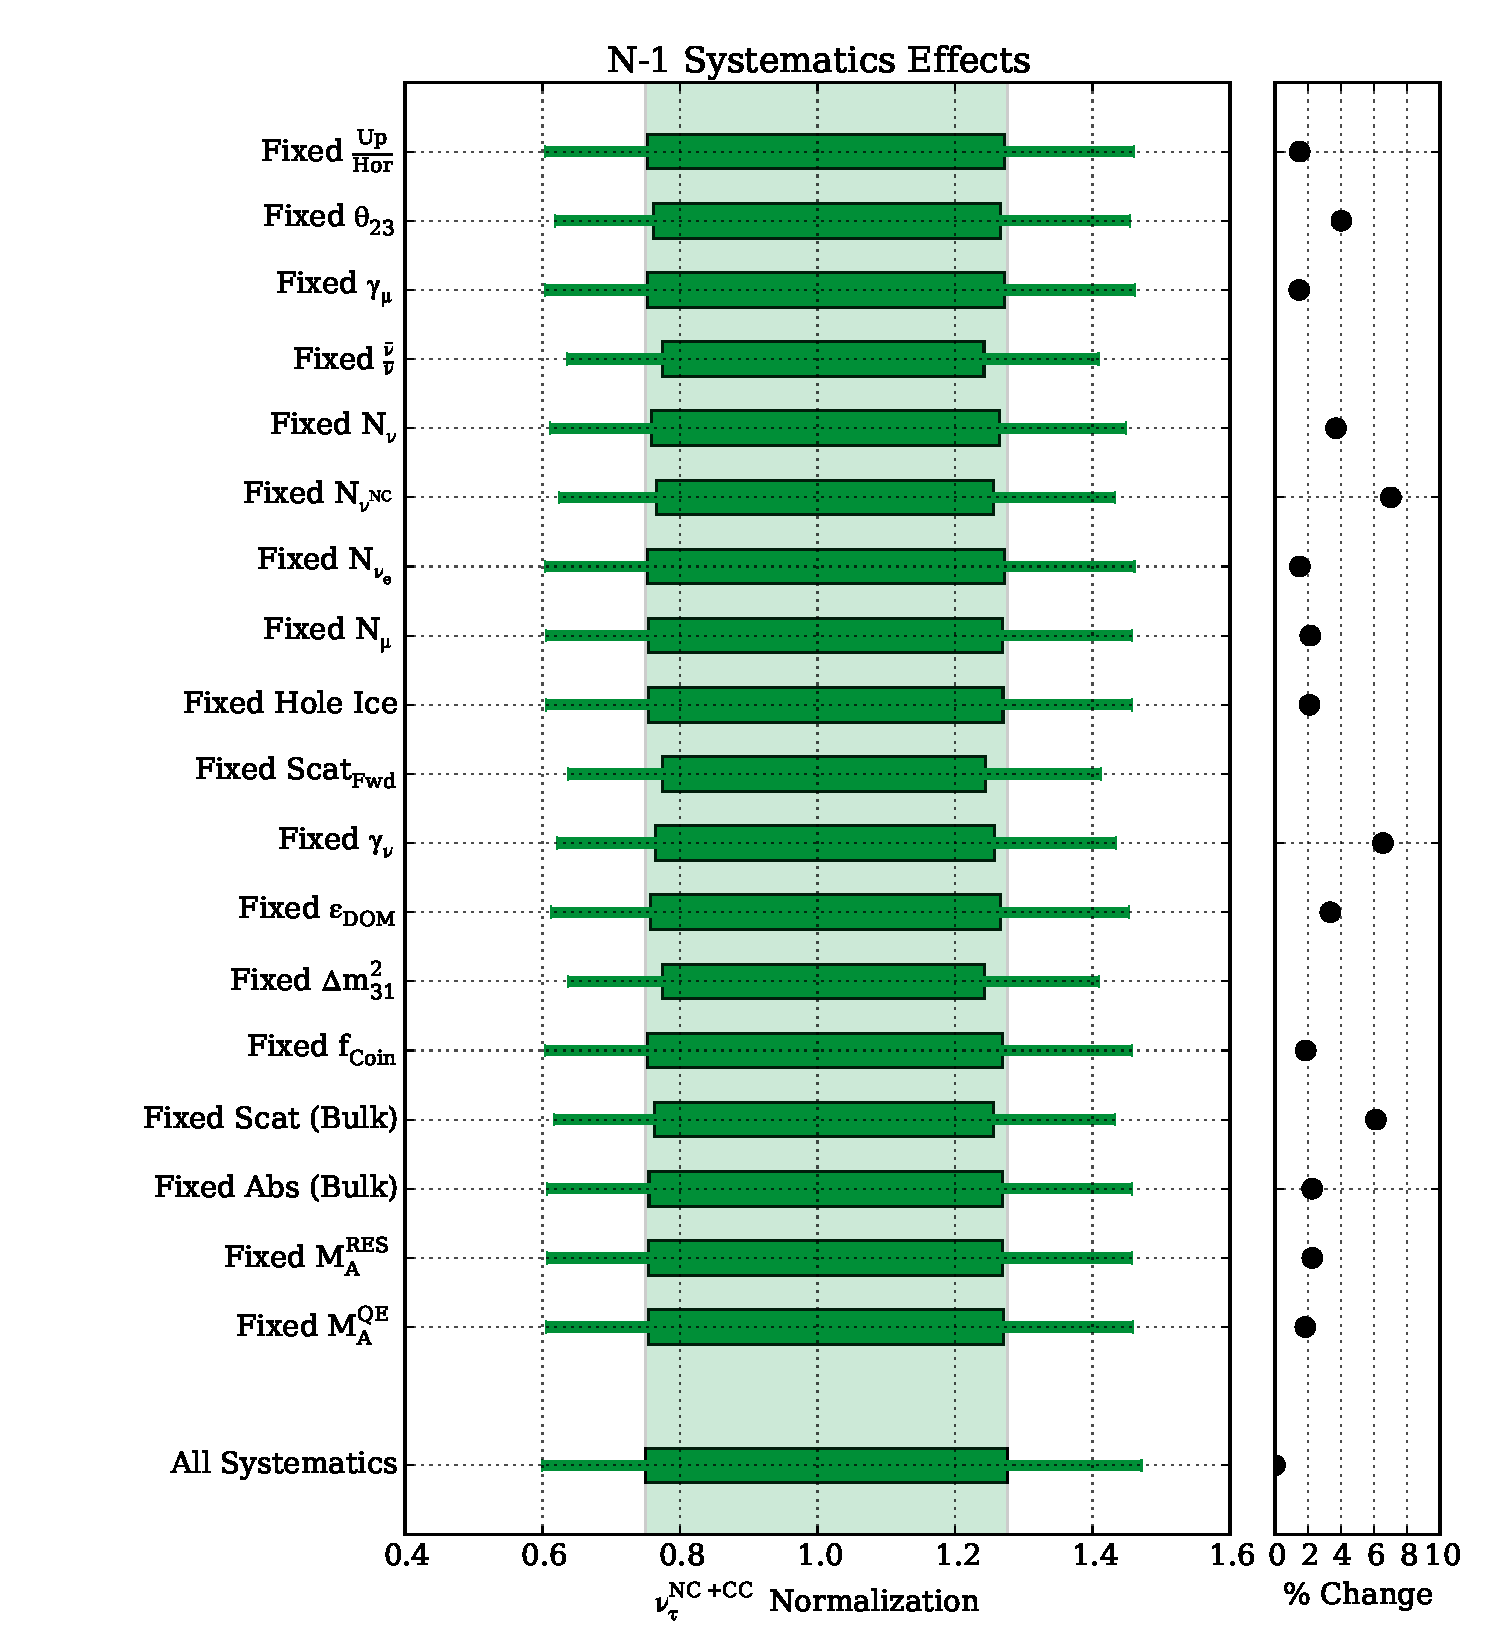
\includegraphics[width=0.45\linewidth]{n-1_widths_nc_cc.pdf} \\
  \small (\textbf{\color{ctcolormain}a}) NC+CC
\end{tabular} \hspace{2pt}
\begin{tabular}[b]{c}
  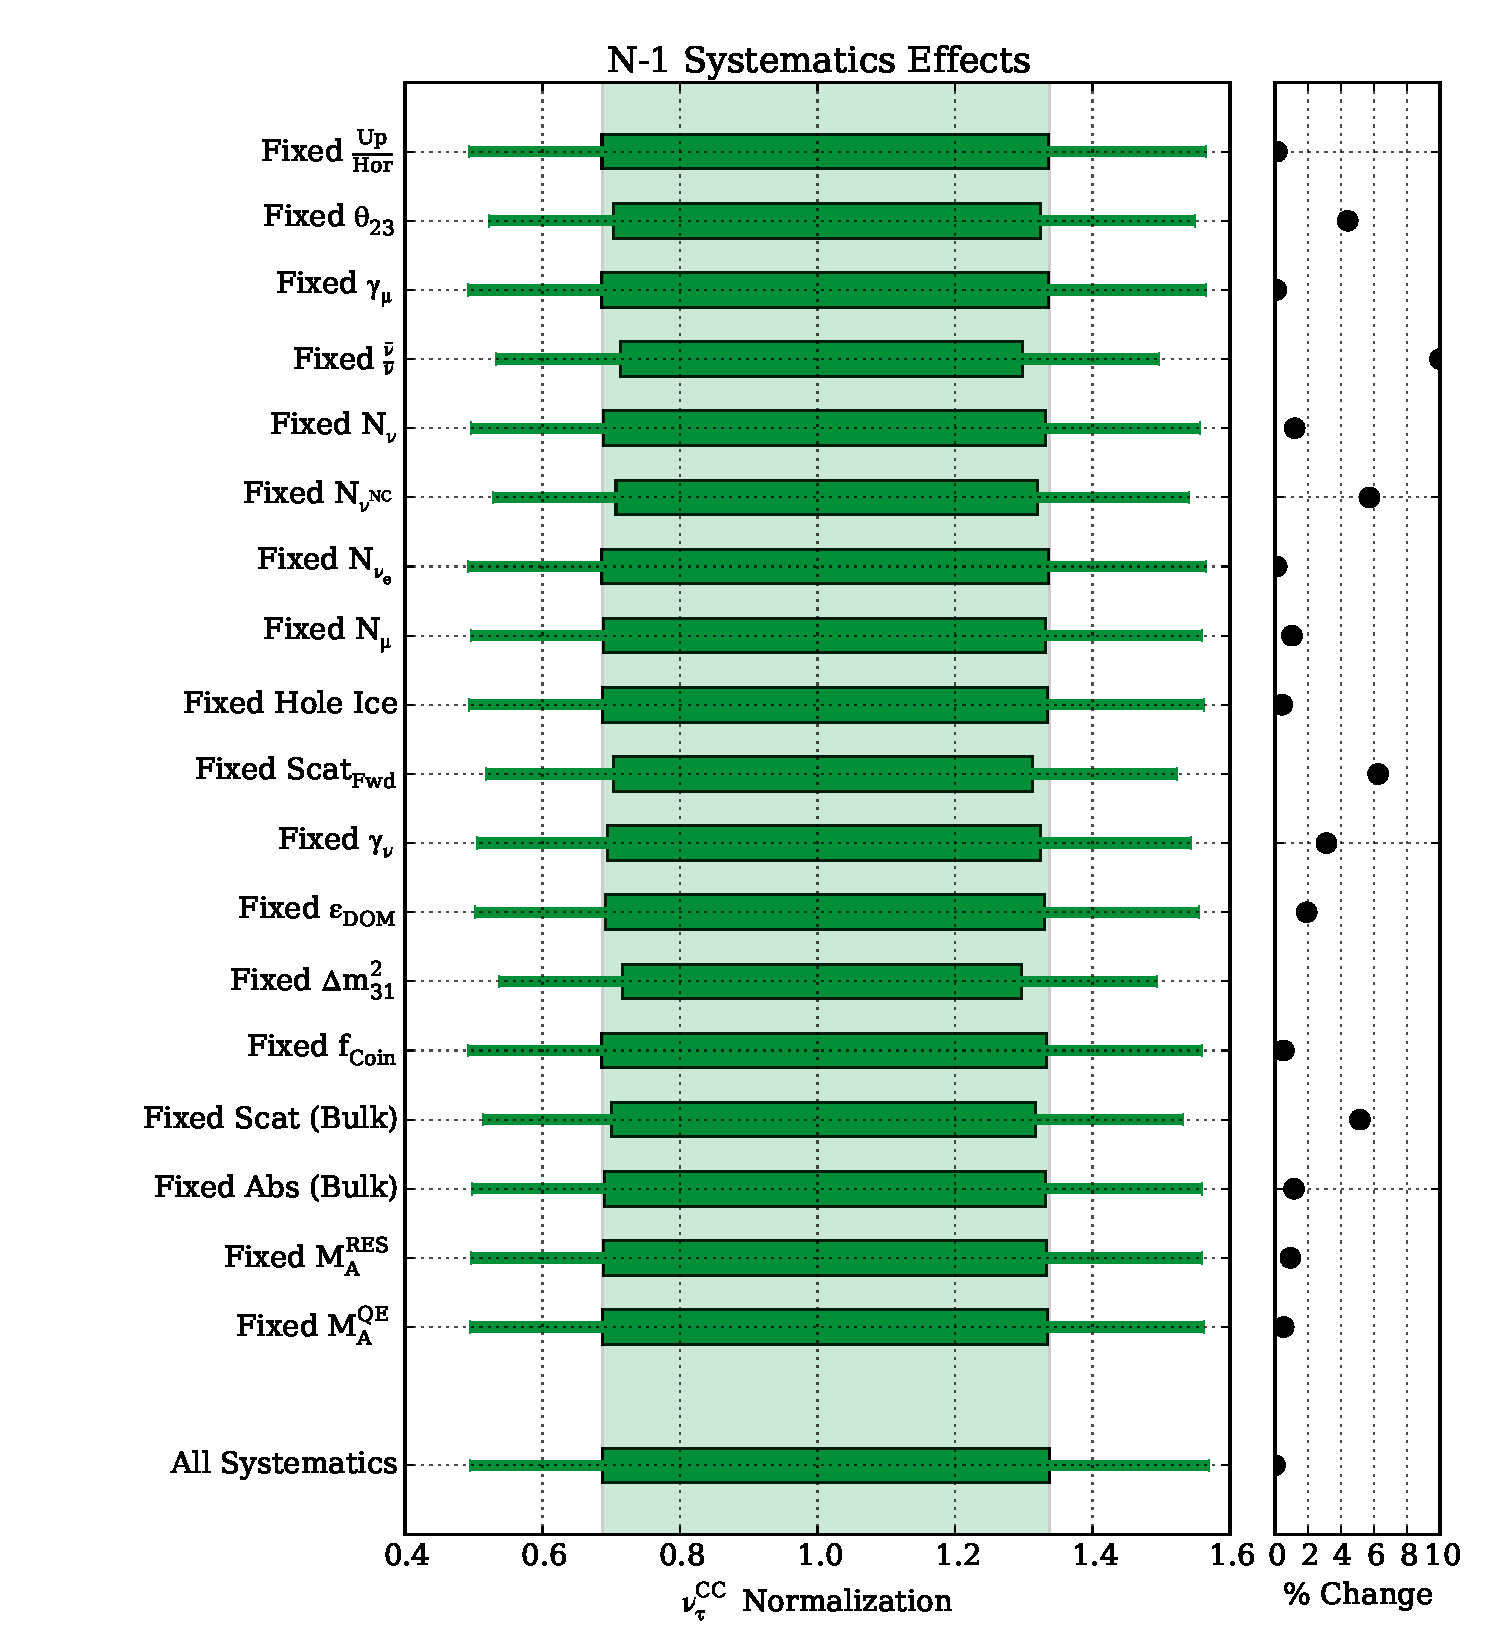
\includegraphics[width=0.45\linewidth]{n-1_widths_cc.pdf} \\
  \small (\textbf{\color{ctcolormain}b}) CC Only
\end{tabular}
\caption[The N-1 redundancy tests]{The N-1 redundancy tests for (a) the NC+CC fit and (b) the CC-only fit. Each parameter is held fixed at the baseline value and the change in the 1$\sigma$ and 90\% expected confidence intervals are tested to identify the most important systematic parameters.}
\label{fig:n-1_tests}
\end{figure}

In contrast to the N+1 tests, N-1 tests start with the full suite of systematics included.
One systematic parameter is fixed to the baseline value and removed from the fit prior to minimization of the $\Delta chi^2$.
The change in the expected result, shown in Figure~\ref{fig:n-1_tests}, allows the investigation of redundancy between systematic uncertainties.
If, for example, two systematic parameters have similar effects in the final histogram, then the N-1 test will show no change in sensitivity due to the removal of one.

The redundancy tests show that the analysis is most strongly affected by the mass splitting $\Delta m^2_{31}$, the $\nu/\bar{\nu}$ ratio, and the forward scattering in the hole ice model.
The up/horizontal ratio, electron neutrino flux normalization, and muon spectral index all have negligible impact in the analysis according to the redundancy tests.

It is also possible that the analysis is strongly sensitive to the value of the systematic and is unlikely to move from the baseline value.
These tests can be useful in identifying redundant parameters for removal, although with the caveat that combinations of parameters are not tested.
After removal of multiple redundant parameters, the updated Asimov sensitivity should be tested once again to verify that the combination of removed parameters remains irrelevant for the fit.
This procedure was used to remove the effects of the DIS uncertainties discussed in Sections~\ref{subsec:xsec_systematics}.
No further parameters have been removed from the tau neutrino appearance fit.

\subsubsection{"Hidden Potential" Tests: Non-Baseline Values}
Both the N+1 and N-1 test suffer from a particular flaw.
Both fail to test the analysis for exceptionally strong sensitivity to particular systematic uncertaintiess.
In order to identify these parameters, the "hidden potential" test has been proposed.
In this test, the Asimov sensitivity of the full analysis containing all proposed systematics is used as a baseline.
Each systematic is then fixed, one at a time, off of the baseline value before rerunning the minimization.
The parameters with priors are fixed to one standard deviation from the prior mean.
The change in the sensitivity gives an indirect measure of the strength of the systematic effect in the analysis.
If no change is observed, the parameter is likely to be redundant and may be investigated for removal from the analysis.

\begin{figure}[h]
\centering
\begin{tabular}[b]{c}
  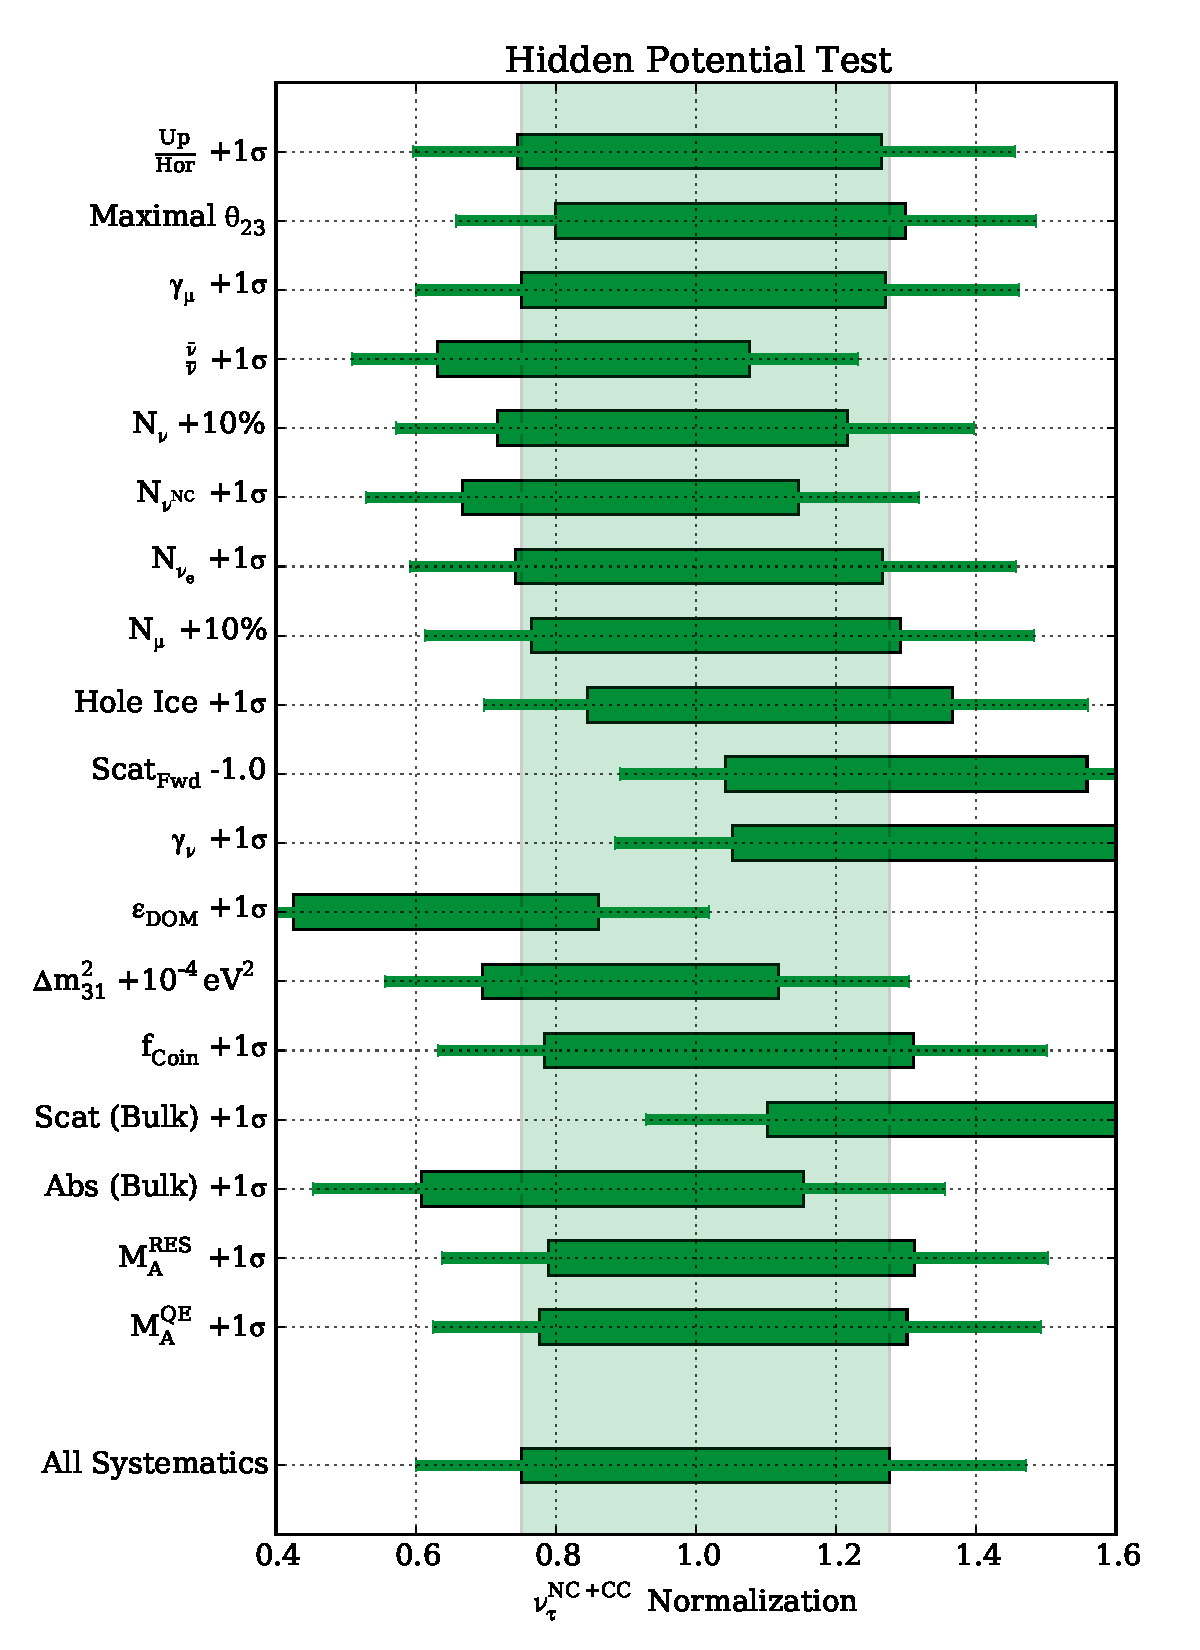
\includegraphics[width=0.45\linewidth]{hidden_widths_nc_cc.pdf} \\
  \small (\textbf{\color{ctcolormain}a}) NC+CC
\end{tabular} \hspace{2pt}
\begin{tabular}[b]{c}
  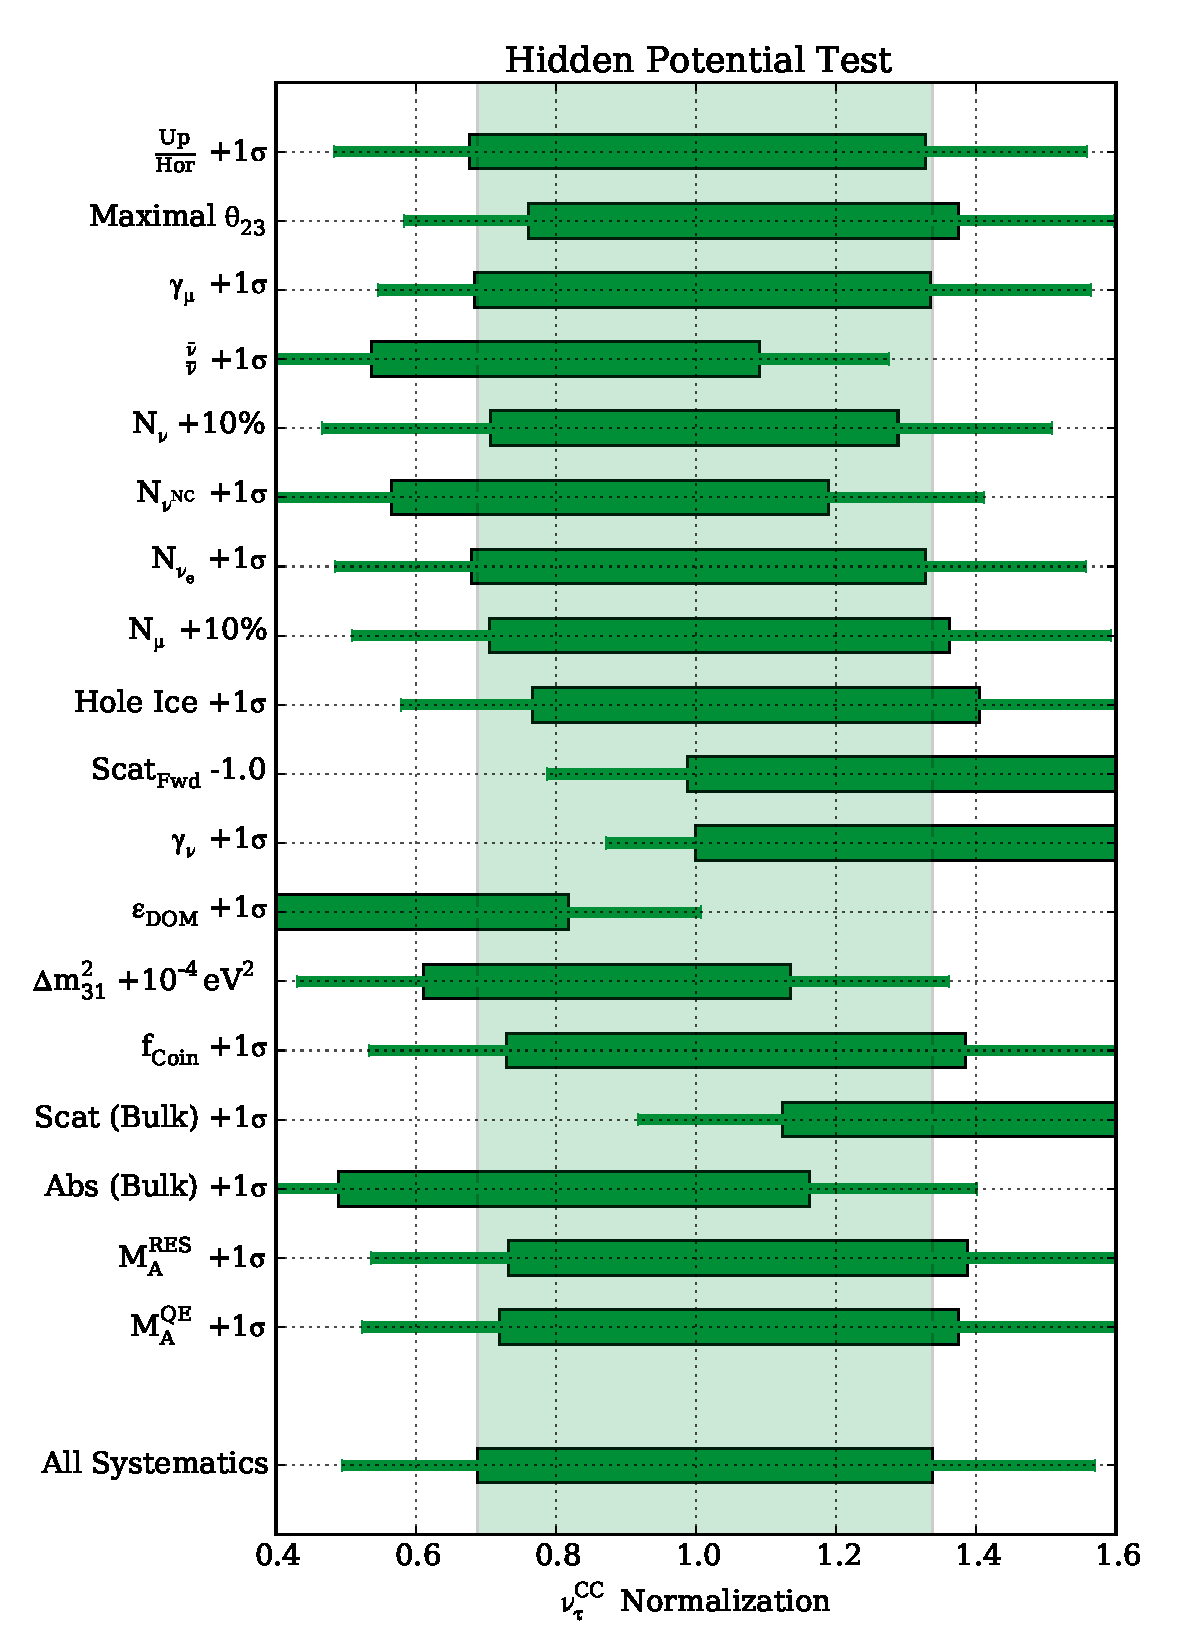
\includegraphics[width=0.45\linewidth]{hidden_widths_cc.pdf} \\
  \small (\textbf{\color{ctcolormain}b}) CC Only
\end{tabular}
\caption[The hidden potential tests]{The hidden potential tests for (a) the NC+CC fit and (b) the CC-only fit. Each parameter is held fixed off the baseline value and the change in the 1$\sigma$ and 90\% expected confidence intervals are tested to identify the most important systematics parameters. If this test shows no impact, mismodeling of the systematic uncertainty has negligible impact on the final analysis.}
\label{fig:hidden_tests}
\end{figure}








\graphicspath{{chapters/analysis/images/}}
\label{sec:fitting_data}
\section{Fitting Data}
Icecube analyses are developed \emph{blindly} in order to minimize bias.
A blind analysis limits potential bias in a measurement by either obfuscating the final measurement parameters or limiting the sensitivity of tests including data.
Oscillation analyses using DeepCore use a staged blind analysis approach.

The initial stage, testing with a small sample of the data to detect software issues, is referred to as a \emph{burn sample} test.
The remaining stages in an IceCube oscillation analysis consist of \emph{blind fits}, where the full dataset is fit while physics parameters are blinded, and the final \emph{unblinding}, in which the best fit parameters are revealed.
These stages will be discussed in turn.

\label{subsec:burn_sample}
\subsection{Burn Sample Fits}
The burn sample used in the search for appearance consisted of 8.7 days of livetime.
A total of 1000 events were found in this burn sample, which was created and tested before the GRECO Level 7 cuts were finalized.

The best fit value of the burn sample was $N^{CC}_{\nu_\tau}$~=~0.
When the normalization was allowed to move into unphysical values of the normalization, the best fit moved to $N^{CC}_{\nu_\tau}$~=~1.23.
One thousand Monte Carlo trials were produced to evaluate the probability of seeing a result more extreme than the unphysical result in the burn sample.
Of the 1000 trials, 14.8\% had a value more negative than -1.23, indicating that this is a common occurance with so little livetime.

Most systematics implemented at the time of the blind fits returned reasonable values.
There was one notable exception: the mass splitting $\Delta m^2_{31}$ returned a value of 3.19~$\10^{-3} eV^2$. 
This value was well inside the expected range for the burn sample fits.
At a value of  $N^{CC}_{\nu_\tau}$=1.0, the mass splitting fit to $\Delta m^2_{31}$~=~2.4~$10^{-3} eV^2$, in good agreement with the global best fit value, 2.526~$10^{-3} eV^2$.





\label{subsec:blind_fits}
\subsection{Blind Fits: Checking the Goodness-of-Fit}
Once the burn sample tests are complete, the next stage is to perform what is known as a \emph{blind fit}.
The concept, developed for oscillation analyses in IceCube, exists as an intermediate stage between the low-sensitivity burn sample tests and the final fit.

Unlike the burn sample fits, the blind fit uses the full data sample for testing.
All systematics are included in the fit.
The final physics parameters, in this case the oscillation parameters, $\Delta m^2_{31}$ and $\theta_{23}$,  and the value of $N_{\nu_\tau}$, are allowed to fit freely, but the final results are restricted and cannot be viewed.
The goodness-of-fit and systematics values are free for investigation.

The blind fit exists in order to identify systematic disagreements between data and simulation.
Investigations of poor agreement are performed blindly without knowledge of the impact on the physics parameters.

Analyzers are free to move onto a request for full unblinding if the goodness-of-fit exceeds 5\%.
If the goodness-of-fit is significantly lower than this limit, the sample and fit must be investigated further to identify any potential issues or oversights.
If no issues are discovered, analyzers can move to a full unblinding request.

The goodness-of-fit, known more informally as the \emph{p-value} associated with the fit, is calculated from an ensemble of Monte Carlo trials.
The fraction of trials with $\chi_{FS}^2$ larger than that observed in data gives the first p-value.

If the fit is particularly poor, a large number of trials may be necessary in order to calculate an accurate p-value.
In these cases, the a $\chi^2$ distribution can be fit to the trials distribution to provide an estimate of the p-value of the fit.



\begin{figure}[h]
\centering 
\begin{tabular}[b]{c}
  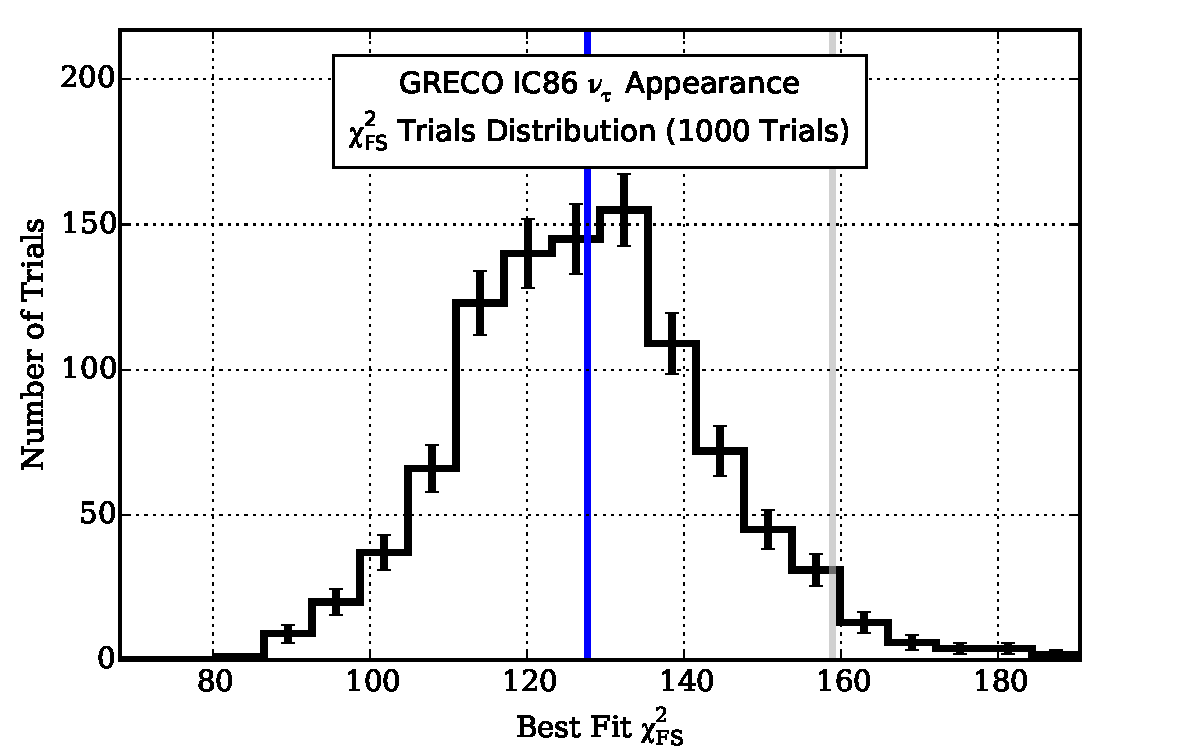
\includegraphics[width=0.45\linewidth]{pvalue_nc_cc.pdf} \\
  \small (\textbf{\color{ctcolormain}a}) NC+CC
\end{tabular} \hspace{2pt}
\begin{tabular}[b]{c}
  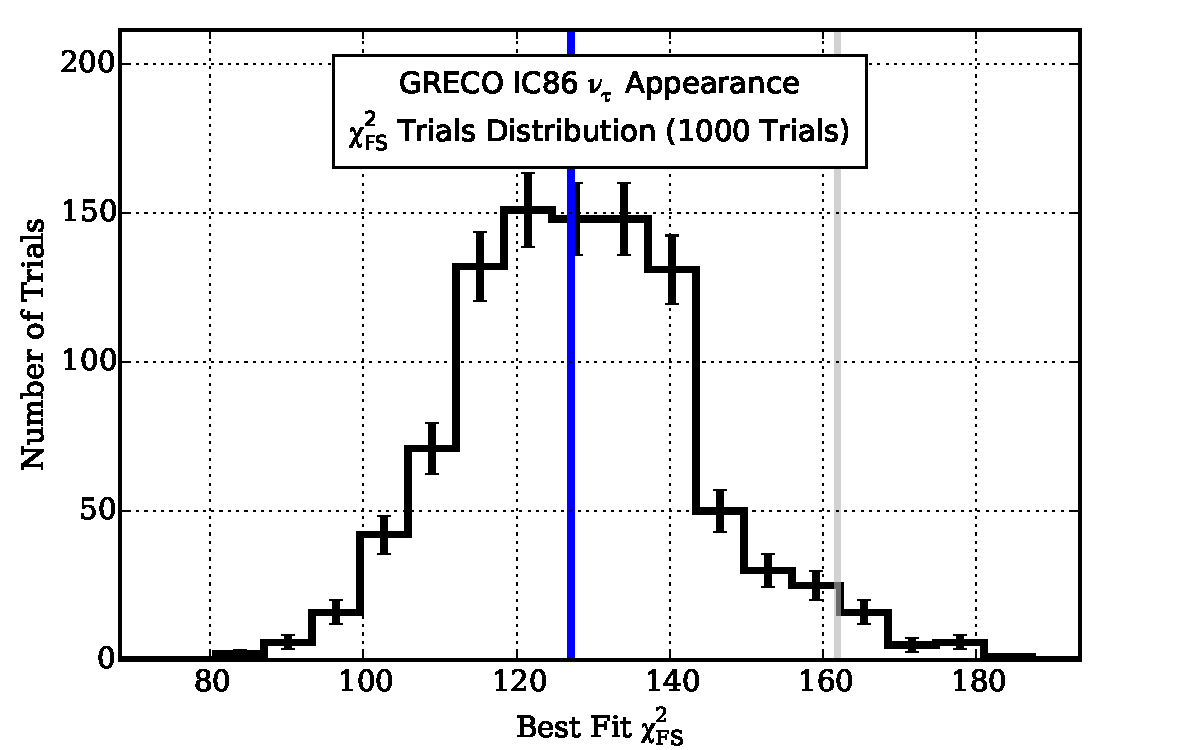
\includegraphics[width=0.45\linewidth]{pvalue_cc.pdf} \\
  \small (\textbf{\color{ctcolormain}b}) CC Only
\end{tabular}
\caption[The goodness of fit in the appearance search]{Goodness of fit in the appearance search. The trials distribution, shown in black, is used to calculate the pvalue. The grey line shows the location corresponding to a 5\% p-value. The blue line shows the value of $\chi^2_{FS}$ found from data. Both fits show good agreement with data and simulation.}
\label{fig:pvalues}
\end{figure}

During the first work with blind fits, this analysis used a wide range of reconstructed energies, including events up to 800 GeV in order to better constrain systematics terms from the non-oscillating higher energy regions.
Blind fits in the GRECO analysis initially showed significant disagreement between the data and simulation, with a goodness-of-fit of ${10^{-7}}$.
Investigations yielded new discoveries, discussed in Section~\ref{sec:greco_discoveries}, about the calibration of both Monte Carlo simulation and data.

After the removal of the flaring DOM events, the correction of bedrock events, and the elimination of the charge in the Pegleg fit, a new blind fit was performed and the goodness-of-fit was again tested.
The resulting $\chi^2_{FS}$ for the charged current only and neutral current + charged current fits were 127.095 and 127.623 respectively.
One thousand trials were run for each fit using the updated sample, yielding estimates of the test statistic distributions.
The p-values, shown in Figure~\ref{fig:pvalues}, were p=52.8\% and  p=49.8\% calculated from trials respectively.
The full map of the ${\chi^2_{FS}}$ values is shown in Figures~\ref{fig:chi2_map_cc} and \ref{fig:chi2_map_nc_cc} in terms of the "signed" $\chi^2$

\begin{equation}
	\chi^2_{Sign} = \sign(d-f)\ \chi^2_{FS}
\end{equation}
%
where $d$ is the data rate and $f$ is the total simulated rate at the best-fit point.

\begin{figure}
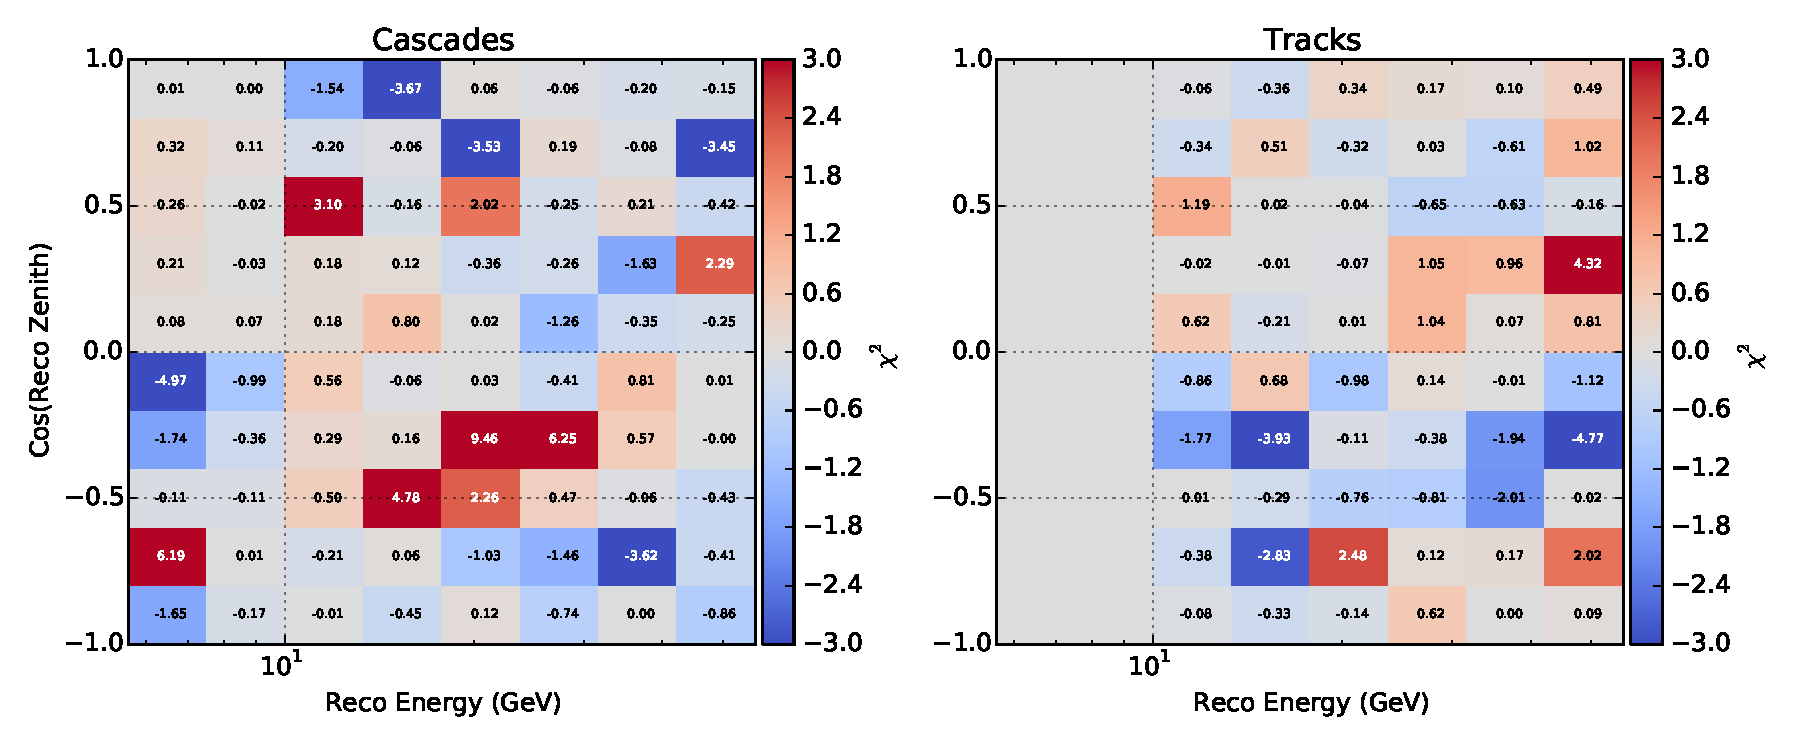
\includegraphics[width=0.9\textwidth]{chi2_map_cc.pdf} 
\caption[The "signed" $\chi^2_{FS}$ values for the CC-only fit]{A map of the "signed" $\chi^2_{FS}$ values for the CC-only fit.}
\label{fig:chi2_map_cc}
\end{figure}

\begin{figure}
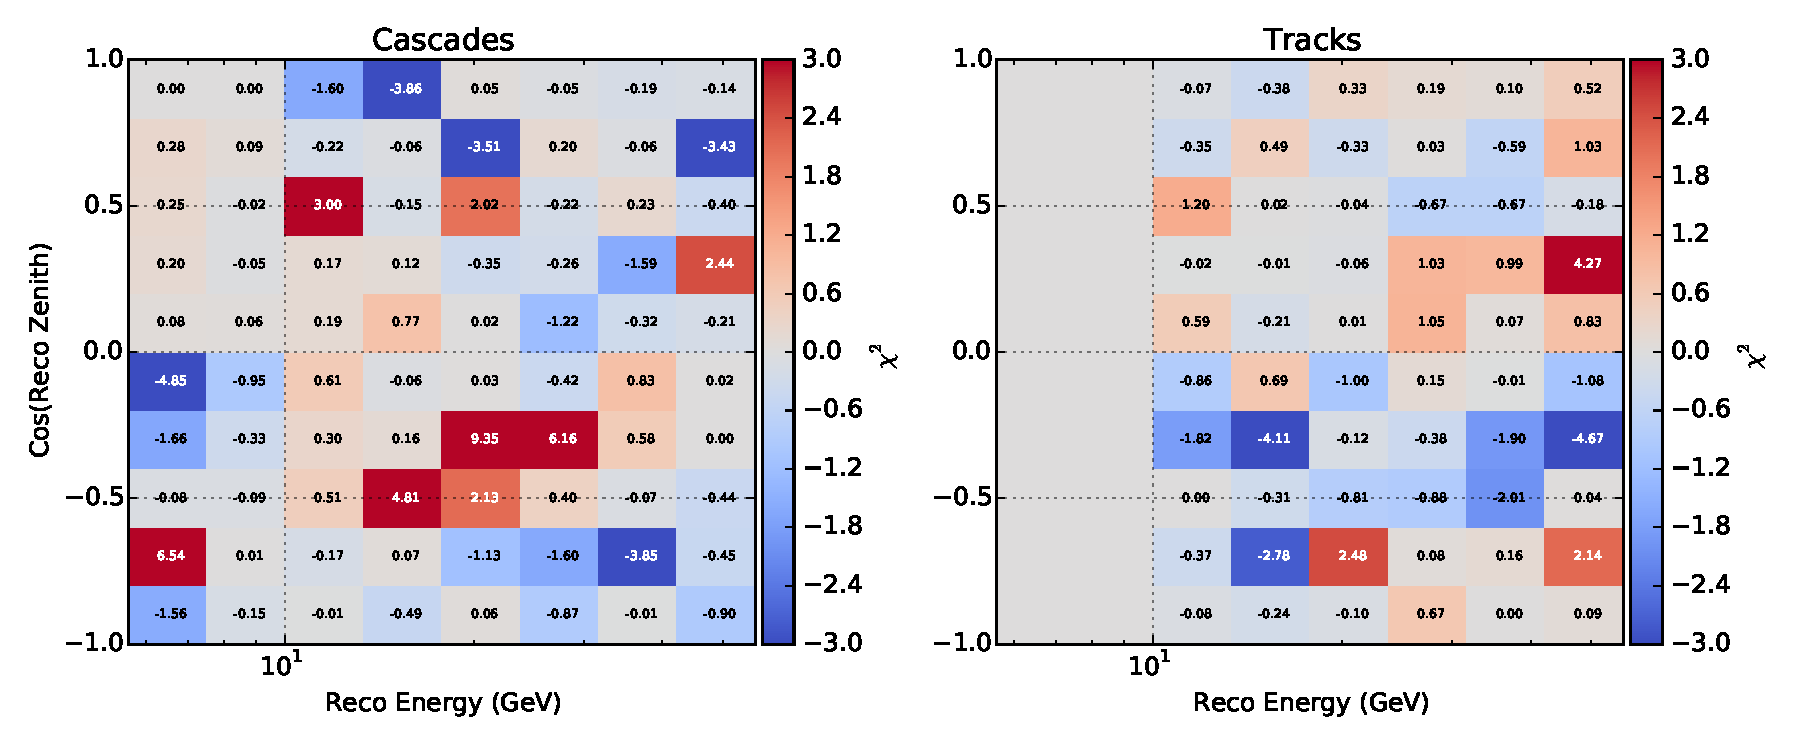
\includegraphics[width=0.9\textwidth]{chi2_map_nc_cc.pdf} 
\caption[The "signed" $\chi^2_{FS}$ values for the NC+CC fit]{A map of the "signed" $\chi^2_{FS}$ values for the NC+CC fit. }
\label{fig:chi2_map_nc_cc}
\end{figure}








\label{section:tau_results}
\section{Results from the Search for Appearance}
With good agreement between data and simulation in the CC-only and CC+NC fits, the appearance measurement with GRECO was granted unblinding approval.
For the fit using only charged current tau neutrino events, the best fit value is $N_{\nu_\tau}^{CC}~=~0.566^{+0.356}_{-0.303}$ (syst+stat).
For the fit including both neutral and charged tau neutrinos, the best fit is $N_{\nu_\tau}^{NC+CC}~=~0.733^{+0.305}_{-0.243}$ (syst+stat).
The intervals are given at the 1$\sigma$ level and include the effects of the Feldman-Cousins procedure.
Both results, shown in Figure~\ref{fig:cc_result} and Figure~\ref{fig:nc_cc_result}, fit lower than expected from unitary 3-flavor oscillations, although both are consistent with such a model.

\begin{figure}
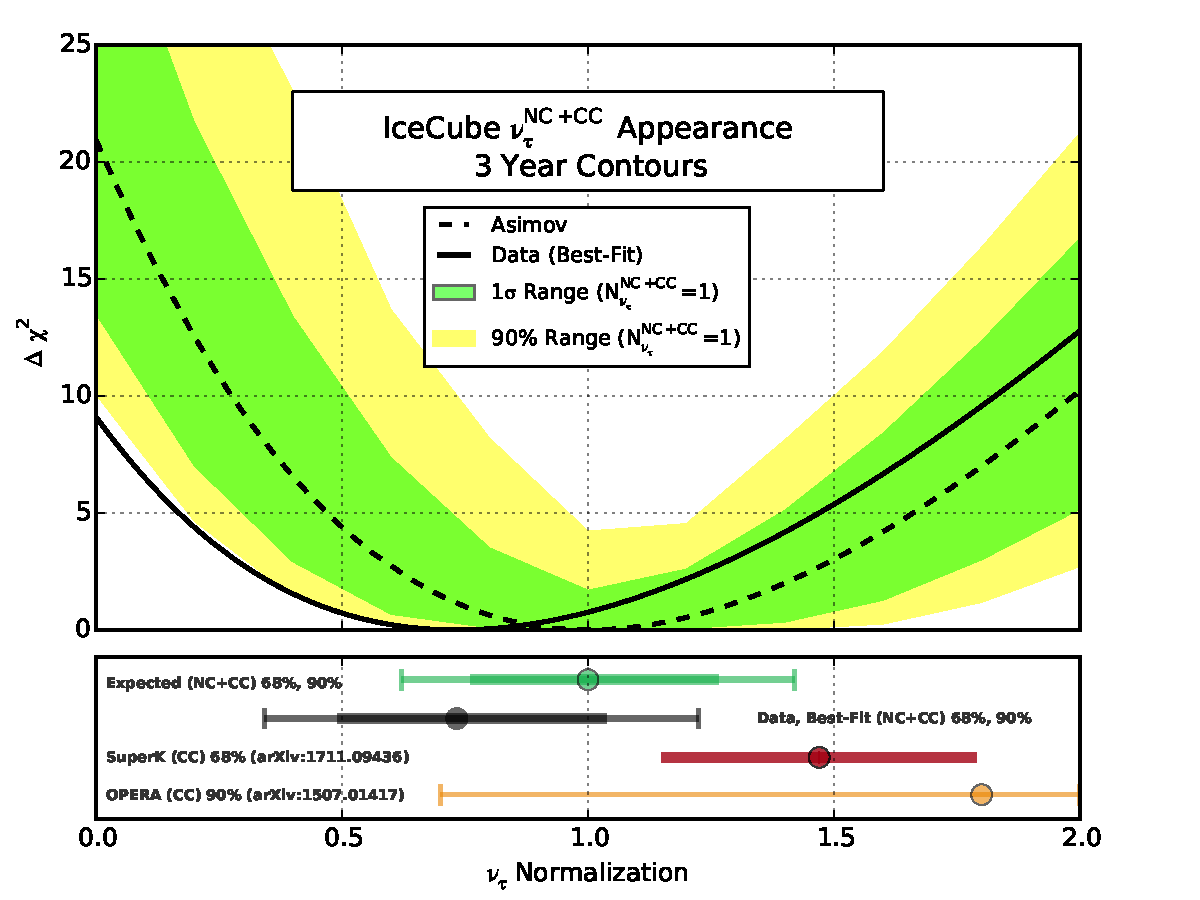
\includegraphics[width=0.9\textwidth]{nc_cc_result.pdf}
\caption[The final result of the CC-only fit]{The final result of the CC-only fit. The best fit is lower than 1.0, at $N_{\nu_\tau}^{CC}=0.566^{+0.356}_{-0.303}$ (syst+stat).}}
\label{fig:cc_result}
\end{figure}

\begin{figure}
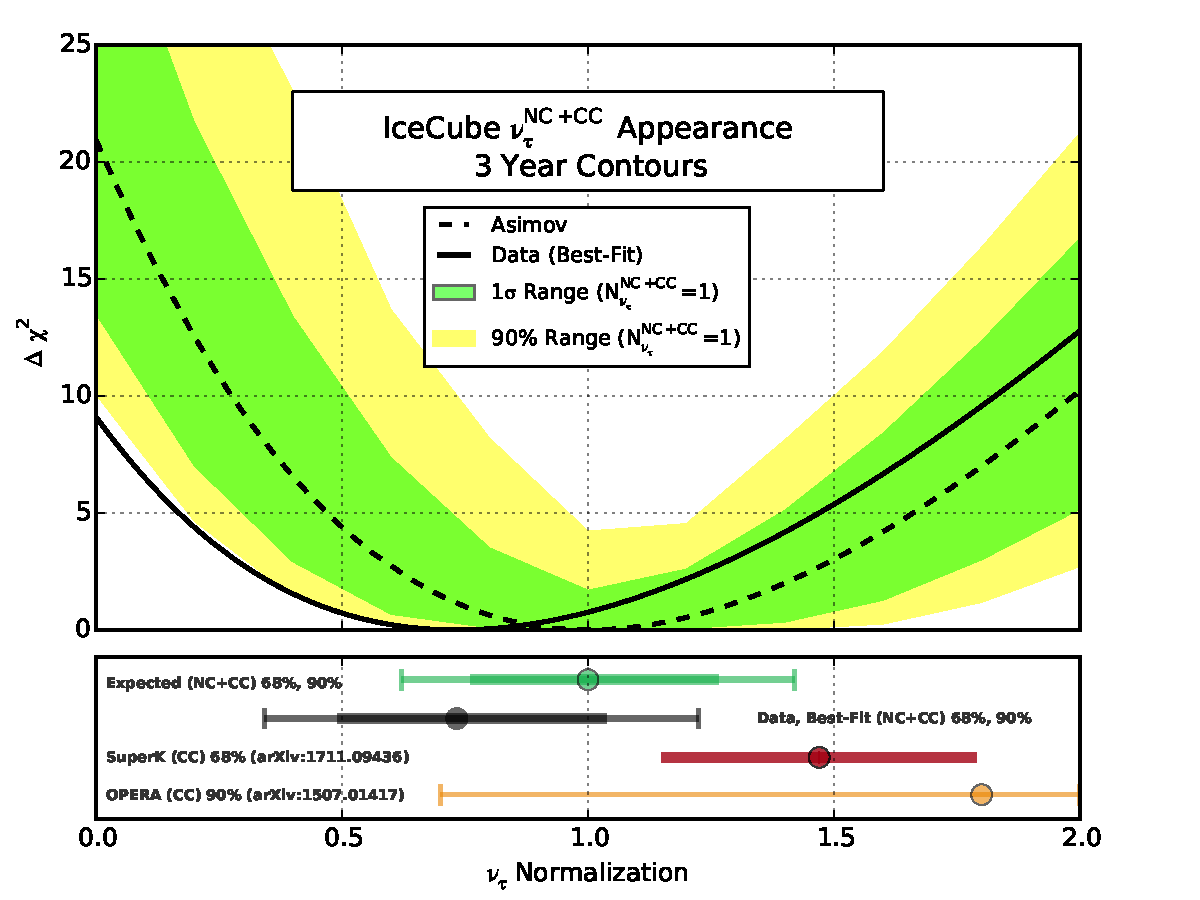
\includegraphics[width=0.9\textwidth]{nc_cc_result.pdf}
\caption[The final result of the NC+CC fit]{The final result of the NC+CC fit. The best fit is lower than 1.0, at $N_{\nu_\tau}^{NC+CC}=0.733^{+0.305}_{-0.243}$ (syst+stat).}
\label{fig:nc_cc_result}
\end{figure}

The final value of the systematics, shown numerically in Table~\ref{tab:bestfit_systematics} and graphically in Figure~\ref{fig:syst_pulls}, are within 1${\sigma}$ of the expectation at the best-fit points.
Many systematics were expected to be determined primarily from the data instead of from priors. 
Figures~\ref{fig:posteriors_cc} and \ref{fig:posteriors_nc_cc} shows the expected values of each systematic parameter measured in 1000 trials.
The shaded band shows the 1${\sigma}$ prior range for each of the parameters, if present.
Not only are all systematics within the relevent priors, but most systematic parameters fit within the expected posteriors as well.

\begin{figure}{}
	\centering 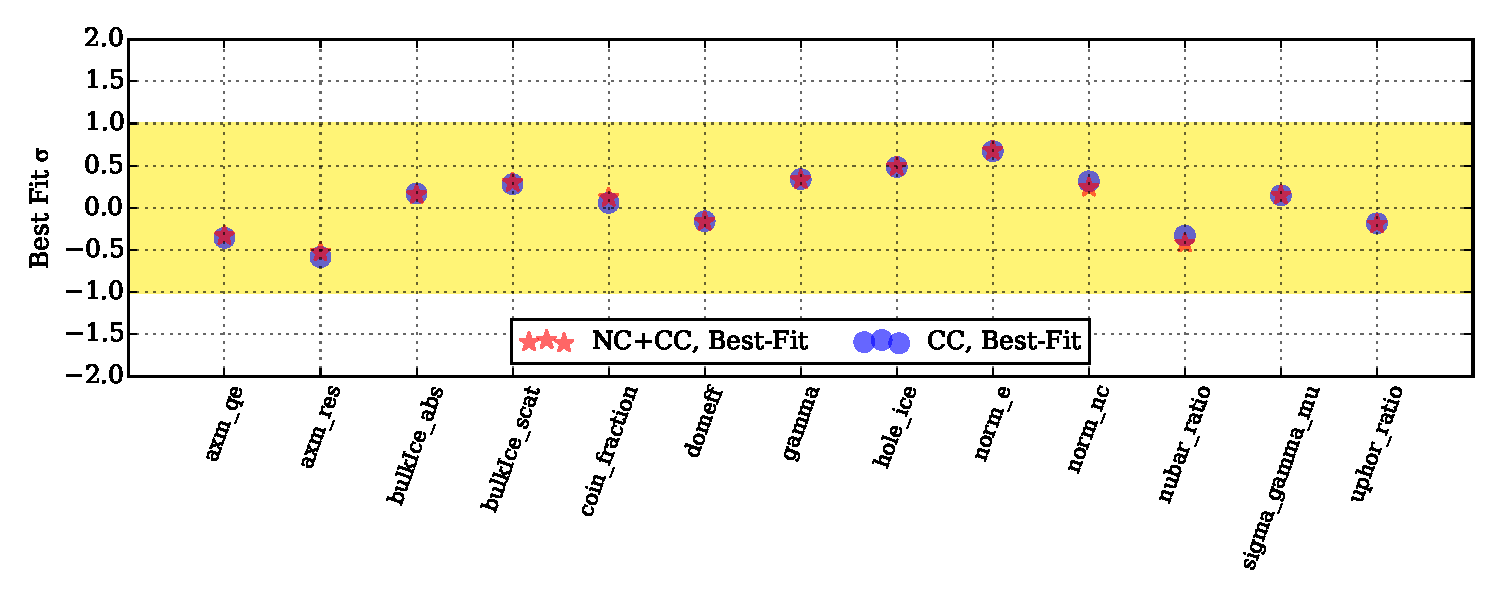
\includegraphics[width=\textwidth]{pulls.pdf}
	\caption[The best fit value of each systematic with priors]{The value of each systematic with priors. The best-fit values are shown for each while the priors are shown by the yellow band. The CC and NC+CC fits are highly correlated, as expected, with very little difference in the systematics best-fit values. All values fit well within the expected 1$\sigma$ ranges.}
	\label{fig:syst_pulls}
\end{figure}

\begin{figure}{}
	\centering 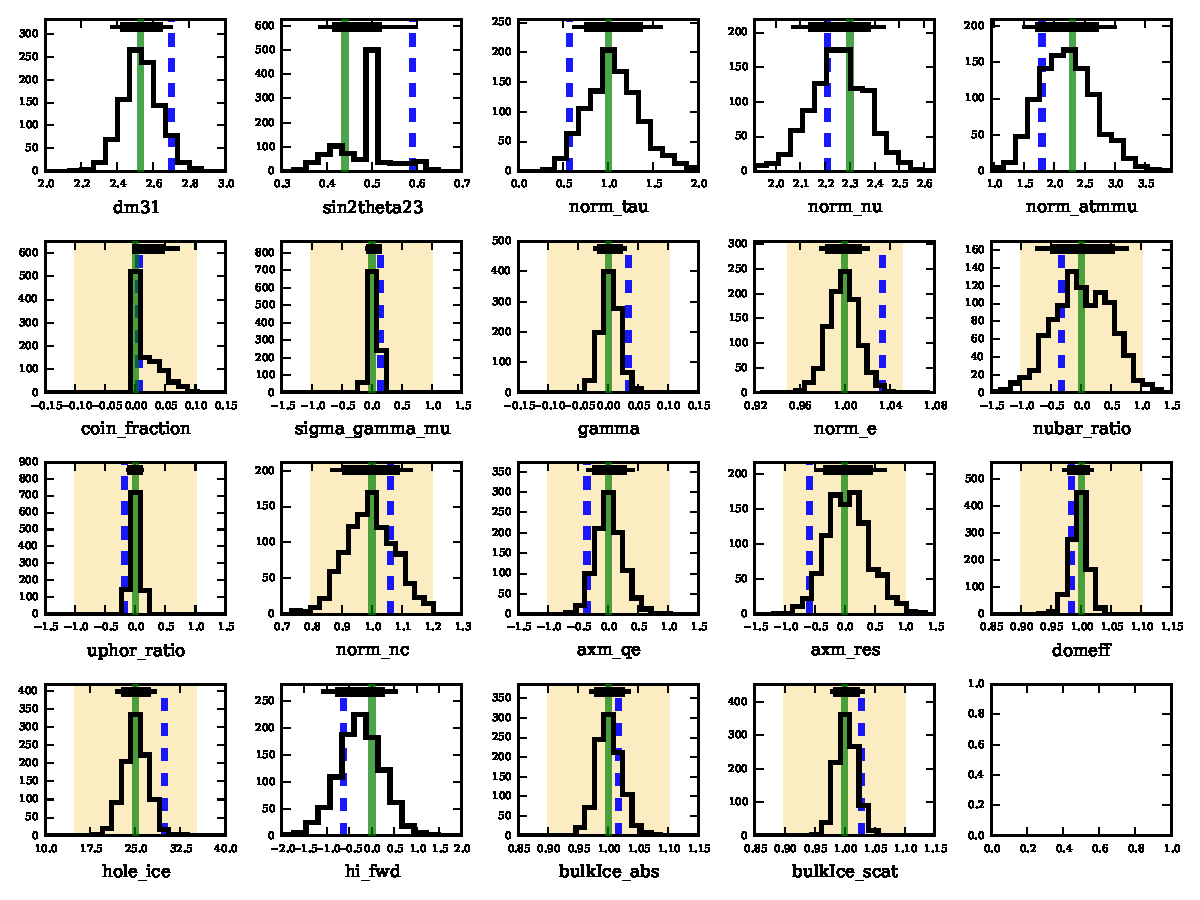
\includegraphics[width=\textwidth]{cc_systematics.pdf}
	\caption[The CC-only posterior distributions expected compared to final fit values]{A comparison of the posterior expected from trials to the final data fit value for each parameter for the CC-only fit. The trials used to build the posterior distribution in each parameter assume baseline values for systematics, $N_{\nu_\tau}^{CC}=1$, and Nu-Fit 2.2 values \cite{NuFit_2.2}. The green vertical line shows the true injected value. The blue dotted line shows the best-fit value from data. The black bar shows the 1$\sigma$ and 90\% ranges calculated from the posterior distribution.}
	\label{fig:posteriors_cc}
\end{figure}

\begin{figure}{}
	\centering \includegraphics[width=\textwidth]{nc+cc_systematics.pdf}
	\caption[The NC+CC posterior distributions expected compared to final fit values]{A comparison of the posterior expected from trials to the final data fit value for each parameter for the NC+CC fit. The trials used to build the posterior distribution in each parameter assume baseline values for systematics, $N_{\nu_\tau}^{NC+CC}=1$, and Nu-Fit 2.2 values \cite{NuFit_2.2}}
	\label{fig:posteriors_nc_cc}
\end{figure}

\begin{landscape}
\begin{table}[]
\centering
\resizebox{\textwidth}{!}{%
\begin{tabular}{@{}lllllll@{}}
\toprule
\multirow{2}{*}{Parameter Type} & \multirow{2}{*}{Fit Parameter}    & \multirow{2}{*}{Units} & \multirow{2}{*}{Prior} & \multicolumn{1}{c}{\multirow{2}{*}{Disappearance}} & \multicolumn{2}{l}{Appearance} \\
                                &                                   &                &             & \multicolumn{1}{c}{} & CC-Only        & NC+CC         \\ \midrule
Oscillations               & $\Delta m^2_{32}$     & $10^{-3}$ $eV^2$ & -        & 2.548           & 2.625          & 2.602         \\
                                & $\sin^2 \left(\theta_{23}\right)$  & -          & -        & 0.576           & 0.590          & 0.584         \\ 
                                & $N_{\nu_\tau}$                   & -               & -                      & 1.0 (Fixed)    & 0.566          & 0.733         \\\midrule
Cross-section            & Axial Mass (QE)           & $\sigma$  & 0 $\pm$ 1.0    & -0.250          & -0.357         & -0.332        \\
                                & Axial Mass (RES)         & $\sigma$   & 0 $\pm$ 1.0   & -0.3737        & -0.583         & -0.526        \\
                                & $N_{NC}$                  & -                & 1 $\pm$ 0.2   & 1.016           & 1.063          & 1.048         \\ \midrule
Neutrino Flux             & $\nu_\mu$ Norm       & Years         & -                     & 2.151           & 2.210          & 2.219         \\
                                & $\nu_e$/$\nu_\mu$  & -               & 1 $\pm$ 0.05  & 1.031           & 1.034          & 1.033         \\
                                & $\gamma_\nu$          & -               & 0 $\pm$ 0.10  & 0.045           & 0.034          & 0.033         \\
                                & $\nu$/$\bar{\nu}$    & $\sigma$  & 0 $\pm$ 1.0     & -0.700         & -0.330         & -0.422        \\
                                & Up/Hor                       & $\sigma$  & 0 $\pm$ 1.0    & -0.207          & -0.184         & -0.191        \\
                                & $f_{Coincident}$        & \%            & 0 + 0.1            & 0.027           & 0.006          & 0.012         \\ \midrule
Muon Flux                  & $\mu$ Norm              & Years        & -                      & 1.845           & 1.795          & 1.830         \\
                                & $\gamma_{CR}$        & $\sigma$  & 0 $\pm$ 1.0    & 0.113          & 0.148          & 0.148         \\ \midrule
Detector                   & DOM Efficiency            & -               & 1.0 $\pm$ 0.1 & 0.980          & 0.984          & 0.984         \\
                                & Hole Ice                      & -               & 25 $\pm$ 10   & 30.526        & 29.833         & 29.894        \\
                                & Forward Scattering      & -               & -                      & -0.839         & -0.638         & -0.630        \\
                                & Absorption                  & \%           & 1.0 $\pm$ 0.1  & 1.014          & 1.017          & 1.016         \\
                                & Scattering                   & \%           & 1.0 $\pm$ 0.1   & 1.033         & 1.028          & 1.030         \\ \bottomrule
\end{tabular}%
}
\caption[The numerical values of the systematics parameters]{The best-fit systematics values for each systematic parameter in the fit. The corresponding parameters for $N_{\nu_\tau}=1$ (ie, the muon neutrino disappearance fit) are included for reference. The CC-only and NC+CC fits are highly correlated, as expected. }
\label{tab:bestfit_systematics}
\end{table}
\end{landscape}

The DeepCore results are the first to fit a value lower than expected, with both OPERA and Super-Kamiokande experiments returning results larger than $N_{\nu_\tau}^{CC}=1$.
The results are consistent with unitary oscillations.


\label{section:other_measurements}
\section{Complementary Measurements from This Analysis}

\label{subsec:oscil_results}
\subsection{Oscillation Parameters}
Thanks to significant contributions from others \cite{Thesis-Martin,Thesis-Elim}, dedicated measurements of the atmospheric mixing parameters have also been performed using the GRECO selection.
In these measurements, the value of ${N_{\nu_\tau}}$ remains fixed to unity.
The derived results are therefore directly comparable to results from other oscillation experiments.

\label{subsubsec:disappearance_results}
\subsubsection{$\nu_\mu$ Disappearance Results}
\begin{figure}
\centering
\includegraphics[width=\textwidth]{michael_contours_external.pdf} 
\caption[The results of a disappearance fit with GRECO]{The results of a muon neutrino disappearance measurement with the GRECO event selection. The new result, shown in blue, fits a larger value of the mass splitting than the most recent published IceCube results \cite{IceCube-Oscillation2018}, shown in blue. The GRECO dataset also prefers a value away from maximal mixing, $sin^2\theta_{23}=0.5$, a first for a DeepCore measurement. The GRECO results are competitive with dedication oscillation measurements from other experiments.}
\label{fig:greco_disappearance}
\end{figure}

Using similar tools as the appearance analysis, a complementary search for ${\nu_\mu}$ disappearance was performed \cite{Thesis-Elim}.
The measurement of the disappearance parameters, ${\Delta m^2_{3j}}$ and ${\theta_{23}}$, used an identical choice of binning and systematics set as the appearance search described above.
The $\chi^2_{FS}$ statistic was found by minimization with the iMinuit package \cite{iminuit-code,iminuit-paper} across a grid of values arranged linearly in ${\Delta m^2_{3j}}$ and ${sin^2\theta_{23}}$ covering both octants.
At each point, the disappearance parameters were fixed during minimization.
Both the normal and inverted ordering were tested separately.

The result is shown in Figure~\ref{fig:greco_disappearance} compared to previous atmospheric oscillation measurements by IceCube \cite{IceCube-Oscillation2018}, Super-Kamiokande \cite{SuperK-Oscillation2015} and the MINOS experiment \cite{MINOS-Atmo2014}.
Results from accelerator measurements are shown from the ${NO\nu A}$ \cite{NOvA-Oscillation2017} and T2K \cite{T2K-Atmo2017} experiments.
All results show the 90\% contour around the best-fit point.
The GRECO result mildly prefers the normal ordering and the second octant, although maximal mixing (${sin^2\theta_{23}=0.5}$ is well within the best-fit contours.

The GRECO result and previous IceCube results are statistically consistent with one another, although the GRECO result perfers a larger mass splitting.
Global fits, which prefer a value of the mass splitting of ${2.494^{+0.033}_{-0.031}}$ as of the time of this writing \cite{NuFit.org}, favor the new GRECO result over the previous IceCube result.


\label{subsubsec:nmo_results}
\subsubsection{Mass Ordering}
\begin{figure}
\centering
\includegraphics[width=0.8\textwidth]{greco_nmo.png}
\caption[Neutrino mass ordering measurement with GRECO]{The measurement of the neutrino mass ordering with the GRECO event selection. The fit is performed only on upgoing events, but includes contributions from a wider energy range than the measurement of tau neutrino appearance. A weak preference for normal ordering is observed.}
\label{fig:greco_nmo}
\end{figure}
In order to quantify the preference for the mass ordering, a dedicated measurement using the GRECO sample was performed \cite{Thesis-Martin}.
This measurement included differences relative to the appearance and disappearance measurements.
Only upgoing reconstructed GRECO events were included, although the energy range was extended to 3-100 GeV.
All simulation templates were smoothed during the analysis using a dedicated implementation of the kernal density estimation technique implemented in the C++ programming language \cite{Thesis-Schoenen}.
This code, unlike the SciPy KDE implementation used in \ref{sec:kde_filtering}, includes functionality for weighted event samples and variable bandwidth estimation.

The systematics set used in the mass ordering analysis was identical to that of the disappearance measurement, with the value of ${N_{\nu_\tau}}$ fixed to unity.
Systematics included in the mass ordering measurement were applied using a parallel branch of the OscFit code used in the appearance measurement.

Statistical uncertainties arising from the simulation statistics were estimated using a bootstrapping technique included in the KDE implementation.
The test statistic used in the mass ordering measurement was the numerical convolution between the Poissonian uncertainty due to the expected event count and a Gaussian model of the bootstrapped Monte Carlo statistical uncertainty.

Unlike the appearance and disappearance measurements, the neutrino mass ordering is not a continuous parameter. 
The calculation of a final significance proceeds following the method described in \cite{Thesis-Ste}, a full description of which is beyond the scope of this work.
Using GRECO events, a good fit is obtained at the best-fit point with a p-value of approximately 80\%.
A weak preference for the normal mass ordering is found at approximately 0.3${\sigma}$ \cite{Thesis-Martin}.

\label{subsec:implications}
\subsection{Implications and Future Work}
There exist various ways to interpret the value of $N_{\nu_\tau}$. 
The value of the tau neutrino normalizations in the CC-only and NC+CC channels are both consistent with the expected value of 1.0.
The standard 3-flavor oscillation model is not strongly disfavored from the GRECO oscillation result.
The current result does, however, provide some tension with the most recent exclusive result from Super-Kamiokande \cite{SuperK-Tau2017,}, which reported ${1.47\pm0.32}$. 
The GRECO and Super-Kamiokande inclusive results differ by approximately 1.8${\sigma}$, assuming the total uncertainties are added in quadrature.
In practice, various systematics, including the atmospheric mixing angle and mass splitting, are likely correlated between the analyses, implying approximately 2${\sigma}$ of tension between the two results.

This analysis, like previous oscillation analyses produced by IceCube, has known limitations.
The GRECO selection includes only three years of detector data.
The data from those three years are selected using strict criteria that explicitly excludes non-standard runs, including those that are ended prematurely.
These short runs are often otherwise unremarkable, but make up a significant fraction of the uptime of the detector in these years and are potentially useful for analysis.
The addition of these runs would increase the total number of events in the GRECO sample by up to 15\%.
The addition of these events presents a simple way to improve the existing result on relatively short timescales.

The three years of data may also be extended in other ways.
The data was originally collected between April 2012 and May 2015.
Since the beginning of this work, additional years of detector data have been collected.
These additional years of data were not included due to calibration changes in the IC86-5 season, discussed in Section~\ref{subsec:spe_template}, which may lead to disagreement between years.
These updated calibrations have since been applied to the earlier years of detector data as well, leading to a self-consistent dataset of approximately 7 years.

The analysis of these events requires a number of upgrades to the simulation which are ongoing at the time of this work.
New efforts are underway updating the simulated SPE templates to better describe the charge profile observed in the detector.
These new templates are fit to detector data for each DOM and are updated for each year, although the year-to-year variations have proven to be small.
New signal and background simulation is therefore necessary to incorporate these upgrades.
The new simulations are underway, with completion and verification expected within the coming year.
If the new sets show good agreement with data, charge information may be reintroduced to the reconstruction, potentially leading to improvements in the reconstructed resolution of events.

The current GRECO selection was the first oscillation selection in IceCube to succesfully use simulated atmospheric muon background events at analysis level.
The simulated livetime is too limited, at 10 months, to allow for precision measurements using the additional years of data.
While the GRECO selection is efficient at rejecting these simulated muons, additional simulation efforts require vast computational resources.
Future analyses will require significantly larger muon datasets in order to adequately describe backgrounds.

The production of additional events for these analyses will require nearly a factor of 9 more events to reach parity between the expected number of muon events in 7 years of data and the raw Monte Carlo statistics.
If only the standard simulation methods are used, this will require about 1.5 years worth of production time.
While the new sets would include muon bundles, a feature not present during production of this work, the sets may still be limited outside of the DeepCore fiducial volume.

The production of new MuonGun simulation is ongoing with efforts to further develop the KDE prescale simulation methods described in Section~\ref{sec:kde_filtering}. 
The KDE prescale method yields significant reductions to the production time of MuonGun simulation for the GRECO selection when using no DOM oversizing.
This can improve by another 8x further if using a DOM oversizing factor of 3.
This may be a viable option for the production of various systematics sets in order to speed the production of background events.
Additional improvements to the simulation efficiency are possible and will undoubtedly be investigated in the near future.
Even using the improvements described here, however, large muon sets are, for the first time, viable as background models in IceCube oscillation analyses.

Improvements are not only possible in the background simulation, however.
Investigations described in Section~\ref{sec:greco_discoveries} have spawned discussions of the limitations of the current GENIE generatior production scheme.
While GENIE was originally planned to be used solely for very low energy oscillation analyses, the dawn of new event selections such as GRECO spanning wider energy ranges can lead to notable disagreement due to the generation scheme.
To better describe the detector, GENIE generation must be examined to identify unsimulated phase space necessary for further analyses.
The simulation of events below the detector, in both the GENIE generator as well as in future MuonGun background simulations, must be given priority in order to explain the events occuring at the bottom or below the IceCube detector.

Future measurements of the tau neutrino appearance are already underway.
Software updates to the GRECO selection are continuing, with new analyses planned for appearance, disappearance, and other searches for low energy neutrinos.

Future measurements may incorporate an planned detector upgrade.
The measurements and techniques for simulated backgrounds presented here will form an integral part of upgrade efforts.
The GRECO selection may also provide a template for selections using the upgraded detector, significantly improving the sensitivity to future oscillation measurements.




